%%%%%%%%%%%%%%%%%%%%%%%%%%%%%%%%%%%%%%%%%
% Classicthesis Typographic Thesis
% LaTeX Template
% Version 1.4 (1/1/16)
%
% This template has been downloaded from:
% http://www.LaTeXTemplates.com
%
% Original author:
% André Miede (http://www.miede.de) with commenting modifications by:
% Vel (vel@LaTeXTemplates.com)
%
% License:
% GNU General Public License (v2)
%
% General Tips:
% 1) Make sure to edit the classicthesis-config.file
% 2) New enumeration (A., B., C., etc in small caps): \begin{aenumerate} \end{aenumerate}
% 3) For margin notes: \marginpar or \graffito{}
% 4) Do not use bold fonts in this style, it is designed around them
% 5) Use tables as in the examples
% 6) See classicthesis-preamble.sty for useful commands
%
%%%%%%%%%%%%%%%%%%%%%%%%%%%%%%%%%%%%%%%%%

%----------------------------------------------------------------------------------------
%	PACKAGES AND OTHER DOCUMENT CONFIGURATIONS
%----------------------------------------------------------------------------------------

\documentclass[
		twoside,openright,titlepage,numbers=noenddot,headinclude,%1headlines,
	 	footinclude=true,cleardoublepage=empty,
		dottedtoc, % Make page numbers in the table of contents flushed right with dots leading to them
		BCOR=5mm,paper=a4,fontsize=12pt, % Binding correction, paper type and font size
		spanish, % Languages, change this to your language(s)
		]{scrreprt} 
                
% Includes the file which contains all the document configurations and packages - make sure to edit this file
%%%%%%%%%%%%%%%%%%%%%%%%%%%%%%%%%%%%%%%%%
% Classicthesis Typographic Thesis
% Configuration File
%
% This file has been downloaded from:
% http://www.LaTeXTemplates.com
%
% Original author:
% André Miede (http://www.miede.de) with extensive commenting changes by:
% Vel (vel@LaTeXTemplates.com)
%
% License:
% GNU General Public License (v2)
%
% Important note:
% The main lines to change in this file are in the DOCUMENT VARIABLES
% section, the rest of the file is for advanced configuration.
%
%%%%%%%%%%%%%%%%%%%%%%%%%%%%%%%%%%%%%%%%%

%----------------------------------------------------------------------------------------
%	CHARACTER ENCODING
%----------------------------------------------------------------------------------------

\PassOptionsToPackage{utf8}{inputenc} % Set the encoding of your files. UTF-8 is the only sensible encoding nowadays. If you can't read äöüßáéçèê∂åëæƒÏ€ then change the encoding setting in your editor, not the line below. If your editor does not support utf8 use another editor!
\usepackage{inputenc}

%----------------------------------------------------------------------------------------
%	DOCUMENT VARIABLES
%	Fill in the lines below to enter your information into the thesis template
%	Each of the commands can be cited anywhere in the thesis
%----------------------------------------------------------------------------------------

% Remove drafting to get rid of the '[ Date - classicthesis version 4.0 ]' text at the bottom of every page
\PassOptionsToPackage{eulerchapternumbers,listings,drafting, pdfspacing, subfig,beramono,eulermath,parts}{classicthesis}
% Available options: drafting parts nochapters linedheaders eulerchapternumbers beramono eulermath pdfspacing minionprospacing tocaligned dottedtoc manychapters listings floatperchapter subfig

\newcommand{\myTitle}{Termómetro emocional para medir la ira a partir de su fisiología\xspace}
\newcommand{\mySubtitle}{Trabajo fin de máster \\\xspace}
\newcommand{\myDegree}{Máster en Internet de las Cosas\xspace}
\newcommand{\myName}{Adrián Gil Moral\xspace}
\newcommand{\myProf}{Virginia Francisco Gilmartín\xspace}
\newcommand{\myOtherProf}{Marlon Cárdenas Bonett\xspace}
%\newcommand{\mySupervisor}{Put name here\xspace}
\newcommand{\myFaculty}{Facultad de informática\xspace}
%\newcommand{\myDepartment}{Put data here\xspace}
\newcommand{\myUni}{Universidad Complutense de Madrid\xspace}
\newcommand{\myLocation}{Madrid\xspace}
\newcommand{\myTime}{Junio 2020\xspace}
%\newcommand{\myVersion}{Alfa\xspace}

%----------------------------------------------------------------------------------------
%	USEFUL COMMANDS
%----------------------------------------------------------------------------------------

\newcommand{\ie}{i.\,e.}
\newcommand{\Ie}{I.\,e.}
\newcommand{\eg}{e.\,g.}
\newcommand{\Eg}{E.\,g.} 

\newcounter{dummy} % Necessary for correct hyperlinks (to index, bib, etc.)
\providecommand{\mLyX}{L\kern-.1667em\lower.25em\hbox{Y}\kern-.125emX\@}
\newlength{\abcd} % for ab..z string length calculation

%----------------------------------------------------------------------------------------
%	PACKAGES
%----------------------------------------------------------------------------------------

\usepackage{lipsum} % Used for inserting dummy 'Lorem ipsum' text into the template

%------------------------------------------------

%\PassOptionsToPackage{ngerman,american}{babel}  % Change this to your language(s)
% Spanish languages need extra options in order to work with this template
%\PassOptionsToPackage{spanish,es-lcroman}{babel}
%\usepackage{babel}

%\usepackage[spanish,american]{babel}

%------------------------------------------------			

\usepackage{csquotes}
\PassOptionsToPackage{%
%backend=biber, % Instead of bibtex
backend=bibtex8,bibencoding=ascii,%
language=auto,%
%style=numeric-comp,%
style=authoryear-comp, % Author 1999, 2010
%bibstyle=authoryear,dashed=false, % dashed: substitute rep. author with ---
sorting=nyt, % name, year, title
maxbibnames=10, % default: 3, et al.
%backref=true,%
natbib=true % natbib compatibility mode (\citep and \citet still work)
}{biblatex}
\usepackage{biblatex}
 
 %------------------------------------------------

\PassOptionsToPackage{fleqn}{amsmath} % Math environments and more by the AMS 
 \usepackage{amsmath}
 
 %------------------------------------------------

\PassOptionsToPackage{T1}{fontenc} % T2A for cyrillics
\usepackage{fontenc}

%------------------------------------------------

\usepackage{textcomp} % Fix warning with missing font shapes

%------------------------------------------------

\usepackage{scrhack} % Fix warnings when using KOMA with listings package  

%------------------------------------------------

\usepackage{xspace} % To get the spacing after macros right

%------------------------------------------------

\usepackage{mparhack} % To get marginpar right

%------------------------------------------------

\usepackage{fixltx2e} % Fixes some LaTeX stuff 

%------------------------------------------------

\PassOptionsToPackage{smaller}{acronym} % Include printonlyused in the first bracket to only show acronyms used in the text
\usepackage{acronym} % Nice macros for handling all acronyms in the thesis

%\renewcommand*{\acsfont}[1]{\textssc{#1}} % For MinionPro
\renewcommand*{\aclabelfont}[1]{\acsfont{#1}}


%------------------------------------------------

\PassOptionsToPackage{pdftex}{graphicx}
\usepackage{graphicx} 

%----------------------------------------------------------------------------------------
%	FLOATS: TABLES, FIGURES AND CAPTIONS SETUP
%----------------------------------------------------------------------------------------

\usepackage{tabularx} % Better tables
\setlength{\extrarowheight}{3pt} % Increase table row height
\newcommand{\tableheadline}[1]{\multicolumn{1}{c}{\spacedlowsmallcaps{#1}}}
\newcommand{\myfloatalign}{\centering} % To be used with each float for alignment
\usepackage{caption}
\captionsetup{font=small}
\usepackage{subfig}  

%----------------------------------------------------------------------------------------
%	CODE LISTINGS SETUP
%----------------------------------------------------------------------------------------

\usepackage{listings} 
%\lstset{emph={trueIndex,root},emphstyle=\color{BlueViolet}}%\underbar} % For special keywords
\lstset{language=[LaTeX]Tex,%C++ % Specify the language(s) for listings here
morekeywords={PassOptionsToPackage,selectlanguage},
keywordstyle=\color{RoyalBlue}, % Add \bfseries for bold
basicstyle=\small\ttfamily, % Makes listings a smaller font size and a different font
%identifierstyle=\color{NavyBlue}, % Color of text inside brackets
commentstyle=\color{Green}\ttfamily, % Color of comments
stringstyle=\rmfamily, % Font type to use for strings
numbers=left, % Change left to none to remove line numbers
numberstyle=\scriptsize, % Font size of the line numbers
stepnumber=5, % Increment of line numbers
numbersep=8pt, % Distance of line numbers from code listing
showstringspaces=false, % Sets whether spaces in strings should appear underlined
breaklines=true, % Force the code to stay in the confines of the listing box
%frameround=ftff, % Uncomment for rounded frame
%frame=single, % Frame border - none/leftline/topline/bottomline/lines/single/shadowbox/L
belowcaptionskip=.75\baselineskip % Space after the "Listing #: Desciption" text and the listing box
}

%----------------------------------------------------------------------------------------
%	HYPERREFERENCES
%----------------------------------------------------------------------------------------

\PassOptionsToPackage{pdftex,hyperfootnotes=false,pdfpagelabels}{hyperref}
\usepackage{hyperref}  % backref linktocpage pagebackref
\pdfcompresslevel=9
\pdfadjustspacing=1

\hypersetup{
% Uncomment the line below to remove all links (to references, figures, tables, etc), useful for b/w printouts
%draft, 
colorlinks=true, linktocpage=true, pdfstartpage=3, pdfstartview=FitV,
% Uncomment the line below if you want to have black links (e.g. for printing black and white)
%colorlinks=false, linktocpage=false, pdfborder={0 0 0}, pdfstartpage=3, pdfstartview=FitV, 
breaklinks=true, pdfpagemode=UseNone, pageanchor=true, pdfpagemode=UseOutlines,%
plainpages=false, bookmarksnumbered, bookmarksopen=true, bookmarksopenlevel=1,%
hypertexnames=true, pdfhighlight=/O,%nesting=true,%frenchlinks,%
urlcolor=webbrown, linkcolor=RoyalBlue, citecolor=webgreen, %pagecolor=RoyalBlue,%
    %urlcolor=Black, linkcolor=Black, citecolor=Black, %pagecolor=Black,%
%------------------------------------------------
% PDF file meta-information
pdftitle={\myTitle},
pdfauthor={\textcopyright\ \myName, \myUni, \myFaculty},
pdfsubject={\myTitle},
pdfkeywords={Computer science, Psycology, Fisiology, Emotions, Internet Of Things},
pdfcreator={pdfLaTeX},
pdfproducer={LaTeX with hyperref and classicthesis}
%------------------------------------------------
}

%----------------------------------------------------------------------------------------
%	AUTOREFERENCES SETUP
%	Redefines how references in text are prefaced for different 
%	languages (e.g. "Section 1.2" or "section 1.2")
%----------------------------------------------------------------------------------------

\makeatletter
\@ifpackageloaded{babel}
{
\addto\extrasamerican{
\renewcommand*{\figureautorefname}{Figura}
\renewcommand*{\tableautorefname}{Tabla}
\renewcommand*{\partautorefname}{Parte}
\renewcommand*{\chapterautorefname}{Capítulo}
\renewcommand*{\sectionautorefname}{Sección}
\renewcommand*{\subsectionautorefname}{Sección}
\renewcommand*{\subsubsectionautorefname}{Sección}
}
\addto\extrasngerman{
\renewcommand*{\paragraphautorefname}{Absatz}
\renewcommand*{\subparagraphautorefname}{Unterabsatz}
\renewcommand*{\footnoteautorefname}{Fu\"snote}
\renewcommand*{\FancyVerbLineautorefname}{Zeile}
\renewcommand*{\theoremautorefname}{Theorem}
\renewcommand*{\appendixautorefname}{Anhang}
\renewcommand*{\equationautorefname}{Gleichung}
\renewcommand*{\itemautorefname}{Punkt}
}
\providecommand{\subfigureautorefname}{\figureautorefname} % Fix to getting autorefs for subfigures right
}{\relax}
\makeatother

\renewcommand{\figurename}{Figura}
\renewcommand\tablename{Tabla}

%----------------------------------------------------------------------------------------
\usepackage{classicthesis} 
%\usepackage[left=0.5in,right=0in,top=0in,bottom=0in]{geometry}
%----------------------------------------------------------------------------------------
%	OWN PACKAGES
%----------------------------------------------------------------------------------------
\usepackage{amssymb}% http://ctan.org/pkg/amssymb
\usepackage{pifont}% http://ctan.org/pkg/pifont
\newcommand{\cmark}{\color{green}\ding{51}\color{black}} % Green tick
\newcommand{\xmark}{\color{red}\ding{55}\color{black}} % Red tick
\usepackage{pdflscape} % Allow landscape pages

%----------------------------------------------------------------------------------------
%	CHANGING TEXT AREA 
%----------------------------------------------------------------------------------------

\linespread{1.2} % a bit more for Palatino
    \areaset[current]{415pt}{761pt} % 686 (factor 2.2) + 33 head + 42 head \the\footskip
%\setlength{\marginparwidth}{2em}%
%\setlength{\marginparsep}{2em}%

%----------------------------------------------------------------------------------------
%	USING DIFFERENT FONTS
%----------------------------------------------------------------------------------------

%\usepackage[oldstylenums]{kpfonts} % oldstyle notextcomp
%\usepackage[osf]{libertine}
%\usepackage[light,condensed,math]{iwona}
%\renewcommand{\sfdefault}{iwona}
%\usepackage{lmodern} % <-- no osf support :-(
%\usepackage{cfr-lm} % 
%\usepackage[urw-garamond]{mathdesign} <-- no osf support :-(
%\usepackage[default,osfigures]{opensans} % scale=0.95 
%\usepackage[sfdefault]{FiraSans}

\usepackage{float}

\addbibresource{references.bib}
%\addbibresource[label=ownpubs]{Self_Publications.bib} % Uncomment for optional self-publications

%\hyphenation{Put special hyphenation here}

\begin{document}

\frenchspacing % Reduces space after periods to make text more compact

\raggedbottom % Makes all pages the height of the text on that page

\selectlanguage{spanish} % Select your default language - e.g. american or ngerman

%\renewcommand*{\bibname}{new name} % Uncomment to change the name of the bibliography
%\setbibpreamble{} % Uncomment to include a preamble to the bibliography - some text before the reference list starts

\pagenumbering{roman} % Roman page numbering prior to the start of the thesis content (i, ii, iii, etc)

\pagestyle{plain} % Suppress headers for the pre-content pages

%----------------------------------------------------------------------------------------
%	PRE-CONTENT THESIS PAGES
%----------------------------------------------------------------------------------------

% Title Page

\begin{titlepage}

\begin{addmargin}[-1cm]{-3cm}
\begin{center}
\large

\hfill
\vfill

\begingroup
%\color{Maroon}\spacedallcaps{\myTitle} \\ \bigskip % Thesis title
\color{Maroon}\spacedallcaps{Termómetro emocional para medir la ira} \\
\color{Maroon}\spacedallcaps{a partir de su fisiología} \\
\bigskip % Thesis title
\endgroup

\spacedlowsmallcaps{\myName} % Your name

\vfill


\includegraphics[width=7cm]{Imagenes/escudoUCM} \\ \medskip % Picture


\myTitle
\xspace

\mySubtitle \medskip % Thesis subtitle
\myDegree \\
%\myDepartment \\
\myFaculty \\
\myUni \\ 
Directora: \myProf \\
Colaborador: \myOtherProf \\
\bigskip

\myTime

\vfill

\end{center}
\end{addmargin}

\end{titlepage}
 % Main title page
%\include{Cascaras/Titleback} % Back of the title page
%\cleardoublepage\include{Cascaras/Dedication} % Dedication page
%\cleardoublepage\include{Cascaras/Foreword} % Uncomment and create a Foreword.tex to include a foreword
%\cleardoublepage\include{Cascaras/Abstract} % Abstract page
%\cleardoublepage\include{Cascaras/Publications} % Publications from the thesis page
%\cleardoublepage\include{Cascaras/Acknowledgments} % Acknowledgements page
\pagestyle{scrheadings} % Show chapter titles as headings
\cleardoublepage% Table of Contents - List of Tables/Figures/Listings and Acronyms

%TODO: 2.2.1.1 (comaprativa de pulseras inteligentes) se va de la línea

\refstepcounter{dummy}

\pdfbookmark[1]{\contentsname}{tableofcontents} % Bookmark name visible in a PDF viewer

\setcounter{tocdepth}{3} % Depth of sections to include in the table of contents - currently up to subsubsections

\setcounter{secnumdepth}{3} % Depth of sections to number in the text itself - currently up to subsubsections

%TODO: los enlaces a las secciones están sólo en el número. hacer que también el nombre sea un enlace
\manualmark
\renewcommand\contentsname{Índice}
\markboth{\spacedlowsmallcaps{\contentsname}}{\spacedlowsmallcaps{\contentsname}}
\tableofcontents 
\automark[section]{chapter}
\renewcommand{\chaptermark}[1]{\markboth{\spacedlowsmallcaps{#1}}{\spacedlowsmallcaps{#1}}}
\renewcommand{\sectionmark}[1]{\markright{\thesection\enspace\spacedlowsmallcaps{#1}}}

\clearpage

\begingroup 
\let\clearpage\relax
\let\cleardoublepage\relax
\let\cleardoublepage\relax

%----------------------------------------------------------------------------------------
%	List of Figures
%----------------------------------------------------------------------------------------

\refstepcounter{dummy}
%\addcontentsline{toc}{chapter}{\listfigurename} % Uncomment if you would like the list of figures to appear in the table of contents
\renewcommand\contentsname{Lista de figuras}
\pdfbookmark[1]{\listfigurename}{lof} % Bookmark name visible in a PDF viewer

\listoffigures

\vspace{8ex}
\newpage

%----------------------------------------------------------------------------------------
%	List of Tables
%----------------------------------------------------------------------------------------

\refstepcounter{dummy}
%\addcontentsline{toc}{chapter}{\listtablename} % Uncomment if you would like the list of tables to appear in the table of contents
\renewcommand\listtablename{Lista de tablas}
\pdfbookmark[1]{\listtablename}{lot} % Bookmark name visible in a PDF viewer

\listoftables
        
\vspace{8ex}
\newpage
    
%----------------------------------------------------------------------------------------
%	List of Listings
%---------------------------------------------------------------------------------------- 

%\refstepcounter{dummy}
%\addcontentsline{toc}{chapter}{\lstlistlistingname} % Uncomment if you would like the list of listings to appear in the table of contents
%\pdfbookmark[1]{\lstlistlistingname}{lol} % Bookmark name visible in a PDF viewer

%\lstlistoflistings 

%\vspace{8ex}
%\newpage
       
%----------------------------------------------------------------------------------------
%	Acronyms
%----------------------------------------------------------------------------------------

\refstepcounter{dummy}
%\addcontentsline{toc}{chapter}{Acronyms} % Uncomment if you would like the acronyms to appear in the table of contents
\pdfbookmark[1]{Acrónimos}{Acrónimos} % Bookmark name visible in a PDF viewer

\markboth{\spacedlowsmallcaps{Acrónimos}}{\spacedlowsmallcaps{Acrónimos}}

\chapter*{Acrónimos}
\begin{acronym}[UML]
\acro{ACC}{Aceleración}
\acro{BDHI}{Inventario de hostilidad de Buss y Durkee}
\acro{BVP}{Presión sanguínea}
\acro{DFA}{Análisis de la función discriminante}
\acro{ECG}{Electrocardiograma}
\acro{EDA}{Actividad electrodérmica, también conocido como respuesta galvánica de la piel (GSR)}
%, respuesta electrodérmica de la piel (EDR), reflejos psicogalvánicos de la piel (PGR), respuesta de conductancia de la piel (SCR), respuesta simpática de la piel (SSR) o nivel de conductancia de la piel (SCL)
\acro{EMG}{Electromiograma}
\acro{FKNN}{Método difuso de los k vecinos más cercanos}
\acro{HHT}{Método de transformación de Hilbert-Huang}
\acro{HR}{Ritmo cardiaco}
\acro{IAPS}{Sistema internacional de fotografías afectivas}
\acro{ICG}{Cardiograma de impedancia}
\acro{IN}{Inclinación}
\acro{IOT}{Internet de las cosas}
\acro{IPRI}{Inventario de Pensamientos Relacionados con la Ira y la hostilidad}
\acro{LDA}{Análisis de discriminación lineal}
\acro{MBA}{Modelos de negocio multinivel}
\acro{MBP}{Propagación hacia atrás de Marquardt}
\acro{NFS}{Sistema neurodifuso}
\acro{ORI}{Orientación}
\acro{PA}{Presión atmosférica}
\acro{PDD-NOS}{Trastorno generalizado del desarrollo no especificado}
\acro{PPG}{Fotopletismógrafo}
\acro{PCG}{Fonocardiograma}
\acro{QDA}{Análisis discriminativo cuadrático}
\acro{RF}{Bosques aleatorios}
\acro{RNA}{Redes de neuronas artificales}
\acro{RESP}{Actividad respiratoria}
\acro{SAM}{Maniquíes de Auto Evaluación}
\acro{SFFS}{Selección secuencial flotante hacia adelante}
\acro{SDK}{Kit de desarrollo de software}
\acro{SKT}{Temperatura de la piel}
\acro{SVM}{Máquina de soporte de vectores}
\acro{TEA}{Trastorno del espectro autista}
\end{acronym}  
                   
\endgroup % Contents, list of figures/tables/listings and acronyms
\cleardoublepage
\pagenumbering{arabic} % Arabic page numbering for thesis content (1, 2, 3, etc)
%\setcounter{page}{90} % Uncomment to manually start the page counter at an arbitrary value (for example if you wish to count the pre-content pages in the page count)
\cleardoublepage % Avoids problems with pdfbookmark

%----------------------------------------------------------------------------------------
%	THESIS CONTENT - CHAPTERS
%----------------------------------------------------------------------------------------

\part{Capítulos}

%---------------------------------------------------------------------
%
%                          Capítulo 1 - Introducción
%
%---------------------------------------------------------------------

\chapter{Introducción}

\paragraph{}
En este capítulo, se va a explicar la motivación de este trabajo (~\ref{sec:motivacion}), los objetivos (~\ref{sec:objetivos}) y la estructura del contenido de esta memoria (~\ref{sec:estructuraMemoria}).

%-------------------------------------------------------------------
\section{Motivación}
\label{sec:motivacion}
\paragraph{}
En una consulta clínica en la que se trabaja con personas que presentan problemas diagnosticados por un psicólogo para la gestión de la ira, es importante recapitular los episodios de la vida cotidiana de esta persona en las que el paciente en cuestión ha tenido que gestionar la ira. En esta narrativa, el terapeuta irá realizando una serie de apuntes para luego intentar ayudar al paciente a que, en situaciones venideras, dicha gestión de la ira mejore o siga siendo estable. Este método, aunque se puede complementar con tests de medición de la ira, presenta un problema fundamental que es que no hay manera de ratificar la veracidad de lo que está diciendo el paciente, por lo que, ya sea de manera consciente o inconsciente (incluso se le puede olvidar mencionar algunos de los episodios de ira), puede que el psicólogo acabe dando una serie de pautas al paciente partiendo de unas premisas distintas a las reales. A su vez, las pautas que recibe el paciente para la gestión de la ira puede que no sean útiles, y éste tenga que esperar hasta la siguiente consulta para poder recibir nuevas indicaciones. Por otro lado, la categorización de la utilidad de las pautas suministradas por el terapeuta dependen de la información recibida por el paciente en las consultas, que, como se verá en la sección ~\ref{subsubsec:intervencionPsico}, la información proporcionada por el paciente puede no ser veraz, lo que puede conllevar la realización de un mal diagnóstico del paciente, puesto que el diagnóstico se sustenta en información falaz.

\paragraph{}
En este trabajo fin de máster, se ha diseñado una solución tecnológica que permite discretizar los episodios de ira del paciente mediante la medición de varias de sus constantes fisiológicas con una pulsera inteligente no intrusiva (para no interferir en el estilo de vida del paciente). Esto permitiría a los te-\\rapeutas tener una visión más objetiva de dichos episodios. Por otra parte, esta solución tecnológica identifica las pautas que más ayudan al paciente para mostrarle en episodios venideros más adecuada en cada momento.

\paragraph{}
De esta manera, se tendría un registro preciso de los episodios de ira que ha experimentado el paciente cruzados con las pautas que le han podido ser más útiles así como la fecha y hora concreta del inicio y fin de los episodios. Esto reduce significativamente la dependencia en la versión del paciente, pudiendo de esta manera reconducir la terapia hacia los episodios más significativos recogidos en la aplicación, que en el caso de no llevar la pulsera inteligente el paciente pudiera no recordar.

\paragraph{}
Por otro lado, un factor crucial de la aplicación es la fiabilidad en la medición de estos episodios de ira. Los falsos positivos que podría detectar la aplicación serán detectados en la propia consulta, hablando con el paciente o revisando los comentarios que pueda haber suministrado el paciente a través de la aplicación en el momento en el que se detectó el falso positivo. Esto es así porque cada vez que se le presente al paciente una pauta, este podrá opcionalmente dar información (por escrito o por voz)sobre la utilidad de la pauta proporcionada por la aplicación, lo que permite que en la propia consulta se parta no sólo de la información cuantitativa recogida a través de las constantes fisiológicas, sino también de la información cualitativa provista opcionalmente por el paciente.

%-------------------------------------------------------------------

\section{Objetivos}
\label{sec:objetivos}

\paragraph{}
Los objetivos primarios de este trabajo son los siguientes:
\begin{enumerate}
    \item Creación de dos aplicaciones: una aplicación Android dirigida a los pacientes, en el que se monitorizarán las constantes fisiológicas del paciente y se le recomendarán pautas para reducir su nivel de ira y una aplicación web para los terapeutas, en el que poder acceder al registro de episodios de ira de sus pacientes y poder crear y asignar nuevas pautas para sus pacientes.
    \item La aplicación web, la aplicación Android y la elección de la pulsera inteligente para medir las constantes fisiológicas deben regirse por el principio de diseño orientado al usuario para que la solución final provean a todas las partes de la mejor experiencia de usuario posible.
    \item Lectura de manera continuada de las mediciones de las constantes fi-\\siológicas de la pulsera inteligente por parte de la aplicación de Android.
    \item Almacenamiento en el dispositivo móvil de los registros de las mediciones y detectar si estas se corresponden con episodios de ira.
    \item Cuando se detecte un episodio de ira, La aplicación de Android deberá mostrar pautas para reducir el nivel de ira.
    \item Al mostrar una pauta, la aplicación de Android deberá permitir al paciente introducir comentarios para poder después revisarlos en la consulta y poder discernir falsos positivos y pautas que no han sido útiles.
    \item La aplicación de Android deberá conectarse de manera intermitente con la aplicación web para por un lado, poder almacenar en la base de datos de la web la información relativa a los episodios de ira y, por otro, que la terapeuta pueda enviar al paciente el conjunto de pautas que le aparecerán en la aplicación móvil cuando se detecten episodios de ira.
    \item La aplicación web deberá permitir la autenticación de varios terapeutas con registros de pautas y pacientes independientes entre sí.
    \item Desde la aplicación web, se podrá visualizar los episodios de ira de cada paciente, incluyendo no sólo un histograma con el nivel de ira en cada momento sino también las pautas recomendadas y los posibles comentarios del paciente en cada nivel de ira.
    \item En la aplicación web se podrán asociar y disociar pautas para los distintos pacientes, pudiendo crear y reutilizar grupos de pautas para pacientes con cuadros clínicos similares.
\end{enumerate}

Los dos objetivos principales de este trabajo son que la aplicación que se cree pueda dar información más precisa tanto al terapeuta como al paciente de los episodios de ira acaecidos y, por otro lado, dar información en tiempo real al paciente que le puedan servir para reducir su nivel de ira.

\paragraph{}
Los objetivos secundarios derivados de los dos objetivos principales son los siguientes:
\begin{enumerate}
    \item Utilización de elementos tecnológicos no intrusivos para que la discretiza-\\ción de los episodios de ira del paciente no supongan un estigma ni sean incómodos en términos fisiológicos.
    \item Intentar incrementar lo máximo posible la pendiente de la curva de aprendizaje para evitar, entre otras cosas, que los elementos tecnológicos en sí acaben siendo motivos del aumento de la frustración e ira.
    \item Adecuación del consumo energético de los dispositivos electrónicos al uso cotidiano. Esto es, no es factible requerir al usuario que cargue el dispositivo móvil o la pulsera inteligente cada 20 minutos por un uso intensivo de energía en la solución tecnológica.
    \item Garantizar el derecho a la intimidad del paciente mediante la encriptación de todos los datos relativos a las mediciones fisiológicas. Esto incluye la encriptación en las bases de datos, la encriptación en las comunicaciones entre la pulsera y el dispotivo móvil y entre el dispositivo móvil y la página web.
\end{enumerate}

\section{Estructura de la memoria}
\label{sec:estructuraMemoria}
\paragraph{}
[TODO: esto queda postergado hasta que esté terminada la primera versión de toda la memoria.]
\cleardoublepage % Empty page before the start of the next part
%---------------------------------------------------------------------
%
%                          Capítulo 2 - Estado del arte
%
%---------------------------------------------------------------------

\chapter{Estado del arte}
\label{cap1:estadoArte}

\paragraph{}
En este capítulo, se va a repasar el estado actual de aquellos aspectos de la psicología (sección~\ref{cap1:sec:Emociones}) y la informática (sección~\ref{sec:iot}) relacionados con este trabajo. En el caso de la psicología, se va a comenzar con una introducción a las distintas teorías psicológicas que han pretendido acotar las emociones (sección~\ref{subsec:teorEmoc}), así como los métodos desarrollados para la medición de las mismas en los humanos sin mediciones fisiológicas (sección~\ref{subsubsec:medicionIra1}), como son los cuestionarios. Tras esto, se van a explorar los métodos para la intervención con pacientes con ira disfuncional (sección~\ref{subsubsec:intervencionPsico}). La parte que concierne a los aspectos psicológicos de esta sección finaliza con la fisiología de la ira (sección~\ref{subsubsec:fisioIra}), lo que permitirá su medición mediante una pulsera inteligente. Para aprovechar el trabajo ya realizado en este ámbito, se realizará una revisión de la medición de la ira (~\ref{subsubsection:medirEmocFisio}). Como este trabajo incluye la realización de experimentos con seres humanos, se concluirá la sección psicológica con la suscripción al código deontológico del Consejo General de Colegios Oficiales de Psicólogos de España (sección~\ref{section:codDeonto}).

\paragraph{}
En lo que respecta a la parte informática, se realizará un breve repaso de las aplicaciones de Internet de las Cosas (sección~\ref{subsec:accIntelig}) así como una comparativa entre distintas pulseras inteligentes que se barajaron para la realización de este trabajo (sección~\ref{subsubsec:pulserasInteligentes}) con la correspondiente explicación de la elección final de la pulsera inteligente que se ha utilizado (sección~\ref{subsubsec:comparativaPulseras}).

%-------------------------------------------------------------------
\section{Emociones}
\label{cap1:sec:Emociones}

\paragraph{}
Las emociones se pueden entender como una reacción subjetiva que ocurre como resultado de cambios psicológicos y fisiológicos que influyen sobre el pensamiento y la conducta \citep{psicoemocional} y que constituyen una experiencia afectiva en cierta manera agradable o desagradable \citep{montanes2005psicologia}. De manera adicional, Wundt (\citeyear{wundt1896lectures}) entendía que las emociones podían definirse según las dimensiones agrado-desagrado, tensión-relajación y excitación-calma.

\paragraph{}
En línea con las observaciones de Wundt, más adelante se simplificó dicho modelo a dos variables con las que se podían representar todas las emociones. Este es el método compuesto por el binomio valencia-activación, que presupone que todas las emociones se pueden definir mediante el nivel de agrado-desagrado (valencia) y calma-activación (activación o \textit{arousal}). El autoreporte de la emoción con este modelo se puede hacer utilizando el método \ac{SAM}, con el que el paciente determina el grado de valencia y activación en una escala de 1 a 5, 7 o 9 (el número de posibilidades la establece el profesional en cuestión) ayudado de una serie de maniquíes como los que se pueden ver en las figuras~\ref{fig:valencia-num} y~\ref{fig:activacion-num}.

\begin{figure}[h]
    \centering
    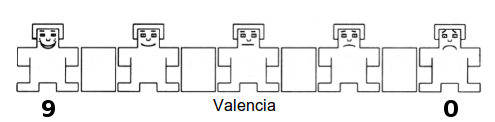
\includegraphics[scale=0.75]{Imagenes/valencia-num}
    \caption[Maniquíes para medir la valencia con el método de SAM extraídos del texto de Hernández (\citeyear{hernandez2016clasificacion}).]{Maniquíes para medir la valencia con el método de SAM (\citep{hernandez2016clasificacion}).}
    \label{fig:valencia-num}
\end{figure}

\begin{figure}[h]
    \centering
    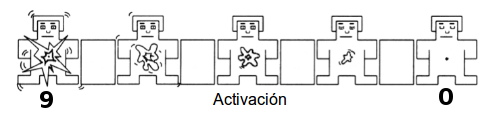
\includegraphics[scale=0.75]{Imagenes/activacion-num}
    \caption[Maniquíes para medir la activación con el método de SAM extraídos del texto de Hernández (\citeyear{hernandez2016clasificacion}).]{Maniquíes para medir la activacion con el método de SAM (\citep{hernandez2016clasificacion}).}
    \label{fig:activacion-num}
\end{figure}

Por tanto, mediante la combinación de la valencia y la activación se pueden representar todas las emociones en ejes cartesianos de dos dimensiones, tal como podemos ver en la figura~\ref{fig:valAct2}.

\begin{figure}[h]
    \centering
    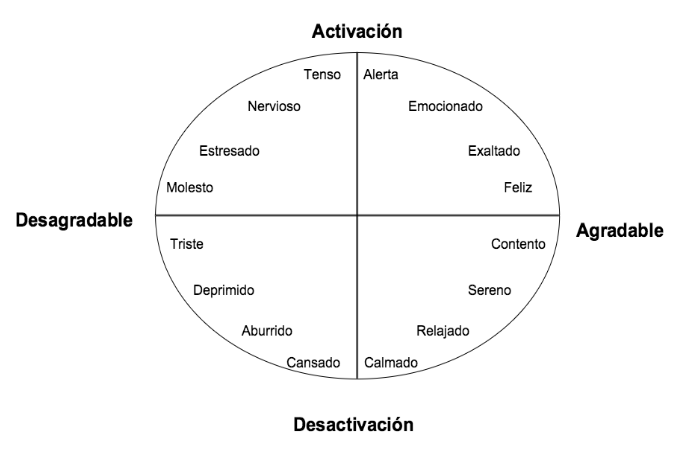
\includegraphics[width=7cm, height=7cm]{Imagenes/valAct2}
    \caption[Representación cartesiana de las emociones utilizando el binomio valencia-activación extraída del texto de Hernández (\citeyear{hernandez2016clasificacion}).]{Representación cartesiana de las emociones utilizando el binomio valencia-activación (\citep{hernandez2016clasificacion}).}
    \label{fig:valAct2}
\end{figure}

%-------------------------------------------------------------------

\subsection{Fundamentos de las emociones}
\paragraph{}
Todas las emociones tienen funciones que permiten tanto la adaptación social como el ajuste personal. Según Reeve (\citeyear{reeve1994motivacion}), la emoción tiene tres funciones principales:
\begin{itemize}
    \item Funciones adaptativas: preparan al organismo para ejecutar eficazmente la conducta exijida para las condiciones ambientales \citep{montanes2005psicologia}. Plutchik (\citeyear{plutchik1980emotion}) establece la siguiente correspondencia entre emociones y su función: miedo - protección; ira- destrucción; alegría - reproducción; tristeza - reintegración; confianza - afiliación; asco - rechazo; anticipación - exploración; sorpresa - exploración. 
    
    \item Funciones sociales: las emociones permiten que otra persona pueda anticipar el comportamiento de quien está expresando una emoción, lo que facilita las relaciones interpersonales. Así, la ira funcional sirve para que un sujeto pueda identificar que está siendo tratado injustamente y de esta manera pueda afrontar la situación con el fin de intentar enmendar dicho desajuste.
    
    \item Funciones motivacionales: la emoción energiza la conducta motivada, haciendo que esta se realice de manera más vigorosa \citep{montanes2005psicologia}. Por ejemplo, la cólera facilita las reacciones defensivas, que al haberse producido una reacción fisiológica previa, permite que las reacciones motoras puedan realizarse con mayor energía que en otro contexto en el que el cuerpo se encontrase en estado de reposo sin sentir dicha emoción.
\end{itemize}

%-------------------------------------------------------------------

\subsection{Teorías emocionales}
\label{subsec:teorEmoc}
\paragraph{}
Las principales corrientes teóricas del estudio de la emoción según Plutchick (\citeyear{plutchik1980emotion}) son:
\begin{itemize}
    \item Evolucionista: iniciada por Darwin (\citeyear{darwin1967expresion}), afirmaba que las emociones evolucionaron porque eran adaptativas y permitían a los seres humanos sobrevivir y reproducirse. Por ejemplo, el miedo impulsaba a la persona a huir o luchar.
    
    \item Psicofisiológica: iniciada por James-Lange (\citeyear{emotionJames}), establece que la fi-\\siología de las emociones precede a las mismas. Siguiendo el ejemplo anterior, este autor establece que no corremos porque tengamos miedo, sino que tenemos miedo porque corremos.
    
    \item Neurológica: iniciada por Cannon-Bard (\citeyear{emotionCannon}), rebate la teoría de James-Lange puesto que las reacciones fisiológicas asociadas a determinadas emociones puede darse sin que entre en acción la emoción correspondiente. Por ejemplo, se puede acelerar el corazón tanto al sentir miedo como al realizar actividades deportivas. Estas teorías se basan en que las emociones se producen como respuesta a un estímulo cuando el tálamo se comunica con el cerebro.
    
    \item Conductista: iniciada por James (\citeyear{james2013principles}), quien defiende en la línea de James-Lange que la reacción fisiológica es previa a la emoción. A su vez, desde esta corriente se entienden las emociones como condicionamientos aprendidos en edades tempranas.
    
    \item Teoría de la activación: iniciada por Schachter-Singer (\citeyear{schachter1962cognitive}), establece primero que la activación fisiológica precede a la emoción y que dicha activación tiene como fin preparar al individuo para situaciones de emergencia.

    \item Teoría cognitiva: iniciada por Lazarus (\citeyear{lazarus1970towards}), establece que son los procesos de valoración cognitiva los que determinan la reacción emocional, por lo que la activación fisiológica por sí sola no desencadena reacciones emocionales. Es decir, quien en última instancia determina la expresión de la emoción es la interpretación que haga el sujeto de la realidad.
\end{itemize}

%-------------------------------------------------------------------

\subsection{Emociones básicas}
\paragraph{}
Las emociones básicas serían aquellas que tendrían un carácter universal, innato y que son distintas entre ellas. A partir de sus combinaciones se podrían generar todas las demás emociones denominadas emociones secundarias o derivadas. Esta teoría es defendida por neodarwinistas como Ekman, Izard y Friesen. Izard (\citeyear{izard1992basic}) establece los siguientes requisitos para que una emoción pueda ser considerada como básica:

\begin{itemize}
    \item Tener un sustrato neural distintivo.
    \item Tener una expresión facial distintiva.
    \item Poseer sentimientos distintivos.
    \item Derivar de procesos biológicos evolutivos.
    \item Manifestar propiedades motivacionales y organizativas de funciones \\ adaptativas.
\end{itemize}

\paragraph{}
Siguiendo este criterio, Izard (\citeyear{izard1992basic}) establecía que las emociones básicas eran: placer, interés, sorpresa, tristeza, ira, asco, miedo y desprecio. Por otro lado, Ekman (\citeyear{ekman1992argument}) considera que las emociones básicas son: ira, alegría, asco, tristeza, sopresa y miedo, lista a la que más tarde añadió el desprecio. Como se puede ver, existe una importante diferencia entre las listas de emociones básicas de ambos autores. Es por ello que autores como Ortony y Turner (\citeyear{ortony1990s}) consideran que no existen emociones básicas ya que ni siquiera entre quienes defienden su existencia, señalan el mismo conjunto de emociones.

\paragraph{}
A continuación se van a describir las características principales de la ira, la emoción con la que se ha trabajado en este proyecto.

%-------------------------------------------------------------------

\subsection{La ira}

\paragraph{}
Las definiciones más extendidas de la ira la catalogan como una emoción que se presenta cuando un organismo se siente bloqueado en la consecución de una necesidad o una meta, sea esta real o fantaseada \citep{nieto2008aproximaciones}. Esta percepción puede ser respondida con un impulso de huida - miedo y ansiedad - o de ataque, en cuyo caso estaríamos hablando de la ira. Esta es una emoción social, que ha servido a lo largo de la evolución para adaptarse a cambios ambientales y activar patrones de actuación útiles para la supervivencia.

\paragraph{}
Actualmente existe un debate abierto respecto a la relación entre este ataque con la agresividad pues no todos los autores catalogan esta emoción como desencadenante de actitudes agresivas; algunos consideran a ésta como la mediadora entre la frustración y la agresión \citep{averill1983studies} mientras que otros señalan la insuficiencia de evidencia experimental para sostener este tipo de afirmaciones \citep{berkowitz1989frustration}.

\paragraph{}
El psicólogo Paul Ekman (\citeyear{ekman1997face}) considera que la expresión facial de esta emoción es universal, al igual que ocurre con el resto de emociones básicas. En la figura~\ref{fig:ekman} se puede ver la cara de una persona al experimentar la ira, cuyos rasgos físicos característicos son: el descenso y la unión de las cejas, la elevación del párpado superior e inferior, la reducción de la apertura palpebral y los labios en tensión, contraídos y apretados \citep{lairama}.


\begin{figure}[h]
    \centering
    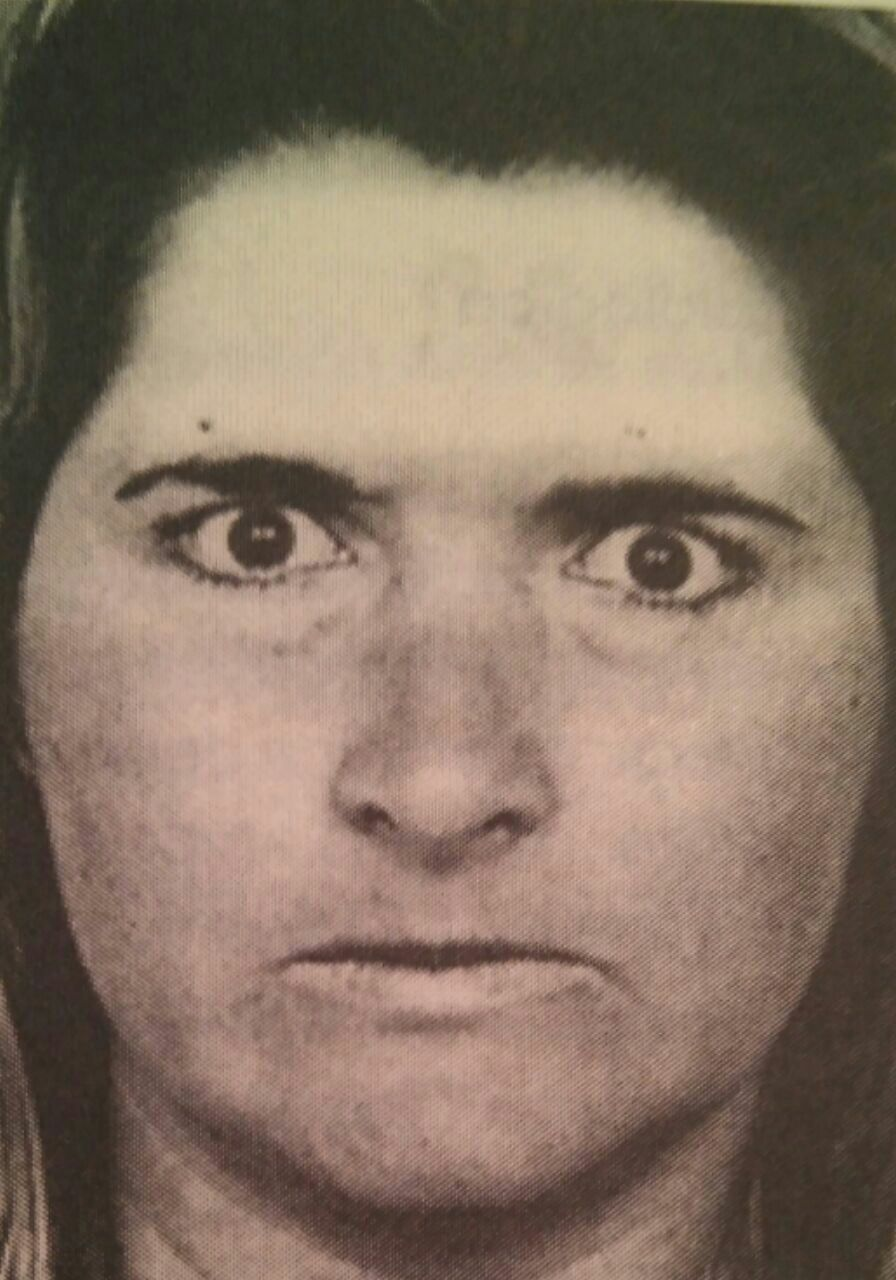
\includegraphics[width=5cm, height=7cm]{Imagenes/ekman-anger}
    \caption[Expresión facial de la ira según se recoge en los FACS de Ekman]{Expresión facial de la ira según se recoge en los FACS de Ekman}
    \label{fig:ekman}
\end{figure}

\paragraph{}
Existen una serie de emociones con una sintomatología similar a la ira: el miedo y la hostilidad. La ira tiende a remover obstáculos que se interponen en la consecución de la meta, mientras que la hostilidad no tiene por qué implicar el acercamiento a la misma. Sus rasgos son la irritabilidad, cinismo e interpretación negativa de las intenciones ajenas. Por su parte, el miedo tiene una sintomatología fisiológica similar a la ira, con la diferencia de que ésta es de menor intensidad en la ira y de que la ira es un sentimiento caliente y el miedo es un sentimiento frío. La diferencia del sentimiento de la ira frente al de frustración es que en la ira el obstáculo en la consecución de la meta es otra persona que además tiene cierta intencionalidad en impedir que se alcance dicho objetivo, mientras que en la frustración no existe dicha intencionalidad ni el obstáculo para alcanzar dicha meta tiene por qué ser externo. Puede ser, por ejemplo, una mala planificación temporal de cara a un examen que se conocía con suficiente antelación para haberlo podido preparar bien.

\subsubsection{Modelo transaccional de la ira}

\paragraph{}
Al categorizar la ira, el equipo de expertos de la universidad de Colorado dirigido por Deffenbacher (\citeyear{deffenbacher2000overcoming}) determinó que la respuesta de esta emoción es regulable y que sólo ocasionalmente y de manera parcial es automática e incontrolable. Para estos autores, la experiencia de la ira podía entenderse como una serie de cinco etapas que irían activándose una tras otra de manera muy rápida, lo que provocaría que la persona no fuera consciente de estar enfadada hasta experimentar la respuesta de la ira. A esta serie de cinco etapas se denomina modelo transaccional de la ira. Estas etapas son las siguientes:

\begin{itemize}
    \item Fase 1 (Estado previo de ira). La personalidad y el estado fisiológico influyen en la expresión de la ira. Por ejemplo, Aaron T. Beck (\citeyear{beck2003prisioneros}) estableció que las personas perfeccionistas, con una mayor necesidad de control, baja tolerancia a la incertidumbre o a la frustración tienden a experimentar la ira con mayor frecuencia e intensidad. A su vez, un experimento de Schieman (\citeyear{schieman2010sociological}) desveló que entre la población estadounidense los rasgos que hacen a una persona propensa a experimentar la ira era ser adultos de entre 30 y 40 años, un bajo nivel educativo, tener varios hijos y tener ingresos bajos. Respecto al estado fisiológico, si la persona tiene sueño o hambre, esto puede hacer que se reduzcan los umbrales de activación de la ira. Esta fase resume los antecedentes que pueden facilitar un episodio de ira, pero por sí sola no tiene que implicar el desencadenamiento de esta emoción.
    
    \item Fase 2 (Procesos de valoración). Como se ha comentado en la definción de la ira, en la experiencia de esta emoción se valora que en una determinada situación se está actuando de manera injusta para con el sujeto. Es en esta etapa en la que se realiza dicha valoración.
    
    \item Fase 3 (Experiencia de la ira). Una vez se ha realizado el proceso de valoración y se ha valorado afirmativamente tanto el trato injusto al sujeto como la intencionalidad en dicho trato, comienzan las reacciones fisiológicas asociadas como pensamientos que se recrean en dicha injusticia, posibles pensamientos de venganza y/o reparación así como otros pensamientos que justifican dicho sentimiento \citep{uceda2011programa}.
    
    \item Fase 4 (La expresión de la ira). En esta fase la ira se activaría de una manera adaptativa para confrontar un problema e iniciar una comunicación recíproca que permita solucionarlo o de manera desadaptativa o disfuncional, que implicaría la violencia verbal o física. 
    
    \item Fase 5 (Consecuencias de la ira). Las consecuencias de la ira dependerán fundamentalmente de si la expresión de la misma ha sido funcional o disfuncional. Si la expresión ha sido funcional, puede que se consiga solventar el problema que se percibía como injusto. En el caso de que haya sido disfuncional, la expresión puede incluso haber empeorado el problema. El motivo por el que se activaría este tipo de expresión de la ira es por dar preferencia al éxtasis del corto plazo durante la expresión frente a las consecuencias futuras en el medio o largo plazo.
\end{itemize}

\subsubsection{Causas de la ira}
%Se hace un salto de línea antes de 'concretas' porque corta mal las sílabas de esta palabra
\paragraph{}
En la mayoría de estudios sobre la ira, esta se suele acotar por el propio paciente mediante cuestionarios en los que bien se presentan situaciones con- \\ cretas que pueden provocar ira, bien se plantean afirmaciones relativas a la ira a las cuales el paciente debe responder en una escala de Likert. Un ejemplo de situación concreta que puede provocar la ira sería ``llegas tarde y el coche que tienes en frente va a 25 kilómetros por hora siendo la limitación de la carretera de 40 kilómetros por hora'', mientras que un ejemplo de afirmación relativa a la ira sería ``tengo ganas de pegarle a alguien''.

\paragraph{}
Por otro lado, en estos cuestionarios las causas que provocan la ira suelen referirse a situaciones muy específicas o demasiado difusas. Como término medio, se puede encontrar el estudio de Alcázar (\citeyear{alcazar2015que}) que versa precisamente sobre las causas que provocan la ira a los estudiantes universitarios. En este caso las fuentes que provocan ira son divididas en tres bloques:
\begin{itemize}
\item Interacción con los demás: mentiras, injusticia, impuntualidad, insultos, irresponsabilidad, traición, discusiones, prepotencia, que alguien diga lo que se tiene que hacer, pelea, hipocresía, ser ignorado, ser contradecido, ser criticado, no ser escuchado, que otra persona cambie los planes...
\item Uno mismo: que no salgan las cosas como se quería, no poder resolver algo, no poder ayudar, trabajar en algo que no se quiere, perder algo, hacer tareas, dormir poco, perder el tiempo...
\item Otros: atascos o retrasos en el transporte público, que deje de funcionar un dispositivo electrónico...
\end{itemize}

Estas situaciones como se puede ver, son bastante genéricas y permiten acotar los motivos que provocan la ira, mientras que en otros estudios que se detallarán más adelante como S.T.A.X.I. o Novaco se intenta únicamente medir la ira.

\subsubsection{Intervención psicológica de la ira disfuncional}
\label{subsubsec:intervencionPsico}

\paragraph{}
A la hora de intentar realizar una intervención efectiva en los casos en los que esté presente la ira disfuncional, es importante saber cuantificar correctamente su intensidad, duración y periodicidad. Para ello, es importante que, además de conocer la sintomatología de emociones similares tal y como se ha mencionado anteriormente, en su medición se tengan en cuenta estos tres factores:
\begin{itemize}
    \item Reactividad situacional: la ira es una emoción social que se da en ámbitos concretos y que depende de cada persona, en la que cada persona aprende los lugares en los que puede o no puede expresar dicha emoción. Es decir, la misma valoración de una situación puede provocar o no la expresión de la ira en la misma persona en función del ambiente y de las personas presentes en ese momento (una persona introvertida por ejemplo puede no sentirse cómoda expresando dicha emoción si esto supone ser el foco de atención). Por ello, para medir esta emoción es importante que la persona se sienta cómoda para poder expresarse emocionalmente como considere, sin provocar situaciones impostadas en el laboratorio en las que debido al ambiente, el sujeto pueda no expresar las emociones tal cual las sienta y de esta manera se evite obtener resultados con baja validez ecológica.
    
    \item Deseabilidad social: es una distorsión inintencionada de la realidad en la que se puede minimizar el problema a la hora de describirlo a terceros (un psicólogo, por ejemplo) por el fin inconsciente de intentar generar una buena imagen en esas personas.
    
    \item Simulación: es una distorsión intencionada de la realidad. Este factor tiene su relevancia en los casos en los que los resultados del análisis puedan tener consecuencias legales sobre el paciente, como pueda ser la presentación de un informe psicológico para un juicio.
\end{itemize}

\paragraph{}
Para evitar caer en alguno de estos errores, es recomendable utilizar enfoques multimétodo-multimomento. En este punto es precisamente en el que accesorios inteligentes no intrusivos pueden ser útiles para obtener datos fia-\\bles fuera de la consulta.


%-------------------------------------------------------------------

\subsubsection{Métodos psicológicos para la medición de la ira}
\label{subsubsec:medicionIra1}

\paragraph{}
Existen numerosas escalas de medición de emociones, en las que no todas ellas han sido validadas. Por ello, se hace especialmente relevante determinar una escala común de confiabilidad, es decir, del grado en que un instrumento de varios elementos mide consistentemente una muestra de la población \citep{celina2005aproximacion}. La escala que se suele utilizar para la medición de la ira es el alfa de Cronbach (\citeyear{cronbach1951coefficient}), que define el grado de correlación existente entre una serie de elementos y aquellos que se quiere medir. Por ejemplo, la correlación entre que el cielo esté nublado y que vaya a llover en la próxima hora es mayor que entre que el día que se quiera saber si va a llover es par o impar, que no tiene ninguna relación con aquello que se pretende inferir, por lo que el hecho de que el dato de si está el cielo nublado o no tendrá un alfa de Cronbach mayor que si el día es par a impar. De la misma manera, se pueden comparar un conjunto de preguntas, que suelen ser denominados métodos o modelos.

\paragraph{}
En el caso que nos concierne, el dato que se quiere inferir es el valor discretizado en el que se encuentra una persona en una escala de de la ira. Cuanto más elevado sea el alfa de Cronbach (en una escala de 0 a 1) para un modelo, mayor será la fiabilidad del mismo. Concretamente, la medición de la ira será desglosada en dos apartados: estado del rasgo de la ira, que evalúa los distintos componentes de la intesidad de esta emoción y su expresión verbal y física y la escala de rasgo de la ira, que mide el temperamento y la reacción de la ira en el sujeto evaluado. 

\paragraph{}
A continuación se citan algunos de los métodos utilizados en psicología para la evaluación de la ira:

\begin{itemize}
    \item S.T.A.X.I. 2 \citep{spielberger}. Es un cuestionario que cuenta con 49 sentencias que miden la experiencia, la expresión y el control de la ira. La escala empleada para responder a las cuestion es de tipo Likert, es decir, incluyen varias opciones según la conformidad con la afirmación realizada (absoluto-mucho, nunca-siempre) a sentencias como ``me siento furioso'' o ``siento que quiero romper cosas''. Estas 49 cuestiones pretenden evaluar al sujeto en los siguientes aspectos: ira en el momento en el que realiza el cuestionario, ira como un rasgo de la persona y por tanto duradero en el tiempo, expresión externa e interna de la ira, control externo e interno de la ira e índice de expresión de la ira, que correlaciona la expresión externa con la expresión interna de la ira. En cuanto a su fiabilidad, en este test obtiene un 0.89 de coeficiente de alfa de Cronbrach en la escala del estado de la ira y un 0.82 en la escala de rasgo de la ira. Este cuestionario ha sido validado para selección de personal e investigación médica \citep{de1997anger, turnage1991job}.

    \item Novaco Anger Inventory \citep{novaco2003novaco}. Es un cuestionario con escala Likert que cuenta con 25 situaciones que pueden provocar la ira en las que se pretende que el sujeto responda el grado de intensidad de la ira que estas provocarían en el sujeto. Algunas de estas situaciones que se plantean son ``alguien ha cometido un error y te culpa'', ``estás intentando discutir algo importante con un amigo o un familiar y no te está dejando la posibilidad de expresar tus sentimientos'' o ``que tu coche se quede atascado en el barro o la nieve''. Este cuestionario ha sido aplicado a adultos que habían cometido infracciones correccionales y entre población con problemas clínicos de gestión de la ira \citep{mills1998novaco, jones1999normative}. En el caso del estudio de Mills, Kroner y Forth (\citeyear{jones1999normative}), el cuestionario de Novaco clasificó correctamente a los pacientes clínicos con una precisión del 94\%. El alfa de Cronbach no se incluyó entre los resultados de validación de este cuestionario.

    \item Inventario de hostilidad de Buss y Durkee (BDHI) \citep{buss1957inventory}. Es un cuestionario de 75 elementos de verdadero o falso que pretenden cuantificar la ira y la hostilidad en sus componentes experienciales y expresivos. Algunas de las cuestiones que se plantean son ``raramente pego a alguien, aun si la persona me pega a mí primero'', ``sé que la gente tiende a hablar mal de mí a mis espaldas'' o ``cuando la gente me grita, yo le grito de vuelta''. Este cuestionario permite medir de forma válida la agresión física y verbal, la ira y la hostilidad en sujetos españoles \citep{lopezvalidacion}. Por otro lado, en un experimento realizado para medir la fiabilidad de este cuestionario, este test obtuvo un alfa de Cronbach de 0.83 \citep{grana2001tipologia}.

    \item Inventario de Pensamientos Relacionados con la Ira y la hostilidad (IPRI) \citep{sukhodolsky2001development}. Es un cuestionario de 26 elementos de tipo Likert que intenta medir la frecuencia en la que el sujeto ha tenido en las últimas semanas pensamientos automáticos asociados a la ira-hostilidad. Las cuestiones están repartidas entre estas cuatro categorías: pensamientos posteriores de ira, pensamientos de venganza, recuerdos que provoquen la ira y el entendimientos de las causas. Algunas de las cuestiones de este cuestionario son ``pienso en los motivos por los que la gente me trata mal'', ``rumio por experiencias de ira pasadas'' o ``recuerdos de molestias pequeñas me molestan durante un tiempo''. En cuanto a su fiabilidad, este cuestionario obtiene un 0.88 de coeficiente de alfa de Cronbach \citep{prieto2000modelo}.
\end{itemize}

\subsubsection{Métodos psicológicos para la intervención con pacientes con ira disfuncional}

\paragraph{}
Una vez se ha evaluado la ira en una persona, en caso de que los resultados obtenidos sean de que ésta se presenta de manera disfuncional, es importante ayudar al paciente a regular esta emoción. A continuación se describen algunas de las propuestas utilizadas para este fin:

\begin{itemize}
    \item Deffenbacher y McKay (\citeyear{deffenbacher1996expression}) proponen un método con los siguientes ejes: aumentar la conciencia del problema mediante preguntas introspectivas, interrumpir el desarrollo de la respuesta de la ira mediante autoinstrucciones, utilizar el entrenamiento por relajación mediante la visualización mental de imagenes que inciten a la calma, reestructuración cognitiva para intentar que los juicios que pueden llevar a la expresión de la ira sean menos dicotómicos y catastrofistas.

    \item Lochman y Wells (\citeyear{lochman1996social}) proponen una mayor concienciación de las seña- \\ les fisológicas asociadas a la ira, aumento de las habilidades sociales para gestionar los problemas de manera más adaptativa y la técnica de tiempo fuera (en caso de no haber conseguido evitar la aparición de la ira de manera disfuncional y ser consciente de ello, alejarse durante unos cuantos segundos de la situación hasta que la reacción fisiológica y cognitiva asociada a la emoción mermen).

    \item Novaco (\citeyear{novaco2003novaco}) propone un enfoque que tiene como ejes principales el aumento de la autoestima del sujeto, pues esto reducirá la probabilidad de que éste responda a provocaciones \citep{rosenbaum1960direct} \citep{veldman1961defensiveness} y aumento no sólo del control de la ira, sino también de la sensación de dicho control, pues de esta manera se aumenta a su vez dicho control de la ira.

    \item Beck (\citeyear{beck1998cognitive}) divide la intervención psicoterapeuta en tres fases. En la primera, denominada fase preventiva, se explica al paciente el \\ funcionamiento de la ira. La segunda, denominada fase de intervención, se centra en los procesos de valoración y en la desactivación fisiológica mediante técnicas de relajación. En la tercera, denominada fase de postvención, en aquellos casos en los que la ira no disminuye, se ahonda en el contexto en el que se da la reacción de la ira.
    
    \item Kendall y Braswell (\citeyear{braswell1985involvement}) se centran en el control de la respuesta impulsiva ante la aparición de problemas, evaluando por tanto en qué medida se preferencia el cortoplacismo a los análisis de medio y largo plazo. Las fases de este modelo son: reconocimiento y definición del problema, desarrollo de alternativas de resolución del problema, focalización de los elementos clave del problema; elección de la solución evitando el cortoplacismo y autorrefuerzo de este modelo resolutivo.
    
    \item Pérez Nieto y Magán Uceda (\citeyear{lairama}) proponen un modelo que consta de nueve etapas distribuidas en tres grandes bloques:
    
    \begin{itemize}
        \item Prevención
        \begin{enumerate}
            \item Cuidar la propia autoestima cuidando las elecciones
            \item Mantener una orientación hacia la tarea.
            \item Identificar escenarios y secuencias habituales de la ira.
        \end{enumerate}

        \item Regulación de la experiencia
        \begin{enumerate}
            \item Identificar las primeras sensaciones (fisiológicas y/o cognitivas) de la ira.        
            \item Reducción de la activación fisiológica.
            \item Revaloración de la relevancia de la situación y de los recursos de afrontamiento.
        \end{enumerate}
        \item Regulación de la expresión y de la respuesta
        \begin{enumerate}
            \item Expresión de deseos personales correctamente, pidiendo, sustituyendo el \textit{tú} por los \textit{mensajes yo}.
            \item Reforzarse por el autocontrol percibido.
            \item Recordar o comentar con otros, más tarde, la gestión que se hizo de la situación conflictiva y lo agradable del autocontrol conseguido.
        \end{enumerate}
    \end{itemize}    
    
    
\end{itemize}

\paragraph{}
Como se puede observar, la mayoría de las propuestas intentan cuantificar las emociones mediante la autoevaluación del sujeto. Según Picard (\citeyear{picard2009future}), los resultados obtenidos por este tipo de técnicas no son fiables (por los factores mencionados en la sección~\ref{subsubsec:intervencionPsico} como la deseabilidad social) pues por un lado un paciente puede no sentirse cómodo expresando dicha emoción con el profesional si no tiene suficiente cercanía, o puede suceder incluso que no entienda alguna pregunta debido a la ambigüedad de la misma. Por ejemplo, en la versión mexicana del cuestionario de S.T.A.X.I. 2, se adaptó el contenido de éste a la jerga mexicana, modificando expresiones respecto a la versión española. El problema es que en su sustitución varias de las frases que se utilizaron eran demasiado similares, por ejemplo: ``me siento enojado'', ``estoy enojado'' y ``estoy ardiendo de enojo'' \citep{oliva2010validacion}.



%-------------------------------------------------------------------

\subsection{Fisiología de las emociones}
\label{subsec:fisioEmoc}

\paragraph{}
Las emociones siempre van acompañadas de reacciones somáticas, siendo las más importantes las alteraciones de la circulación, los cambios respiratorios y las secrecciones glandulares. Los tres componentes de las respuestas emocionales son los siguientes:

\begin{itemize}
    \item Componente comportamental o conductual: incluye todos los movimientos musculares que se desencadenan tras una emoción (en el caso del miedo, la huida o el enfrentamiento, con sus correspondientes movimientos musculares).
    
    \item Componente neurovegetativo: comprende los cambios en el sistema ner-\\vioso autónomo para aportar una rápida movilización de energía que podría ser necesaria en caso de realizar movimientos enérgicos. En el caso del miedo, esto provocaría una activación de la rama simpática -para ganar tensión muscular y actividad cardíaca- y una desactivación de la rama parasimpática -para que la activación se centre en los músculos y no por ejemplo en procesos digestivos-.
    
    \item Componente hormonal: refuerzan las respuestas neurovegetativas mediante la secrección de hormonas como la adrenalina o la noradrenalina.
\end{itemize}

\paragraph{}
En las respuestas fisiológicas de las emociones, la amígdala juega un papel relevante, pues es donde se interpreta la información de las 	aferencias (señales que provienen de las neuronas sensoriales que transmiten información de lo que ocurre en distintas partes del cuerpo así como en el entorno) para redireccionar ésta a la región cerebral correspondiente que producirá la eferencia (respuestas neurológicas del sistema nervioso central tras la interpretación de las aferencias). En la tabla~\ref{tab:respEmoc}, se puede encontrar una lista de ejemplos de regiones cerebrales que reciben aferencias del núcleo central de la amígdala y las respuestas emocionales que controlan estas regiones.

\begin{table}[]
\caption{Regiones cerebrales que reciben aferencias de la amígdala y las respues-\\tas emocionales que controlan esas regiones.\citep{davis1992}}
\label{tab:respEmoc}
\begin{tabular}{|c|c|}
\hline
\textbf{Regiones cerebrales}                                                          & \textbf{\begin{tabular}[c]{@{}c@{}}Respuestas comportamentales\\ y fisiológicas\end{tabular}}                                                  \\ \hline
Hipotálamo lateral                                                                    & \begin{tabular}[c]{@{}c@{}}Activación simpática: aumento de la \\ frecuencia cardíaca y la presión arterial, \\ palidez.\end{tabular} \\ \hline
Núcleo motor dorsal del vago                                                          & \begin{tabular}[c]{@{}c@{}}Activación parasimpática: \\ úlceras, micción, defecación\end{tabular}                                           \\ \hline
Núcleo parabranquial                                                                  & Respiración agitada.                                                                                                                           \\ \hline
Área tegmental ventral                                                                & Alerta comportamental (dopamina).                                                                                                              \\ \hline
Locus coeruleus                                                                       & Aumento de la vigilancia (noradrenalina).                                                                                                      \\ \hline
\begin{tabular}[c]{@{}c@{}}Núcleo reticular de la\\ protuberancia caudal\end{tabular} & Aumento de la respuesta al sobresalto.                                                                                                         \\ \hline
Sustancia gris periacueductal                                                         & Cese de la conducta (congelación).                                                                                                             \\ \hline
\end{tabular}
\end{table}

\paragraph{}
Un elemento importante en la fisiología de las emociones es el aprendizaje de la lectura de las situaciones para poder anticiparse a situaciones que están por venir. Esto puede producirse mediante el aprendizaje de estímulos neutros a los que se le asocia una reacción emocional (es decir, el condicionamiento clásico). Si una perro antes de recibir su comida preferida escucha de manera consistente un timbre y no escucha ese mismo timbre cuando no recibe comida, acabará asociando mediante condicionamiento clásico que el estímulo neutro (el timbre) es ahora un estímulo condicionado que provocará la respuesta fisiológica condicionada equivalente a la respuesta incondicional; esto es, acabará salivando ante la expectativa de la comida al escuchar el timbre antes incluso de detectar la comida. Así, en el caso de los humanos, la mayoría de los miedos se adquieren por transmisión social, en lugar de por exposición directa al estímulo \citep{olsson2007learning}.

\paragraph{}
En lo que respecta a la parte fisiológica que no tiene proyección exterior, existe un campo de estudio llamado psicología de la salud que vincula las emociones con la salud entendida en toda su extensión. Así, las emociones positivas afectan de manera positiva a la salud, sucediendo lo inverso con las emociones negativas, puesto que favorecen la aparición de ciertas enfermedades al hacer más vulnerable al sistema inmunológico \citep{moure2011}. Un estudio de 1999 ya planteaba que las personas que experimentan ansiedad crónica, prolongados periodos de tristeza y pesimismo u hostilidad, tenían el doble de riesgo de contraer enfermedades como el asma, la artritis o los dolores de cabeza \citep{lopez1999}. En el caso de la ansiedad, esta puede complicar una operación médica, puesto que la reacción fisiológica que provoca es la dilatación de las venas provocando por tanto sangrados más abundantes \citep{moure2011}. En cuanto a las emociones positivas, la risa disminuye la concentración del cortisol, que es una de las hormonas directamente vinculadas al estrés, lo que potencia la actividad de los linfocitos, responsables de una correcta respuesta inmunológica \citep{berk2008cortisol}.

\paragraph{}
Todos estos parámetros se miden tras la normalización de los mismos en función del sujeto en cuestión. Una técnica habitual es establecer primeramente el valor de las variables que se quieren medir en un estado de reposo para luego compararlo con los valores a la hora de someter al sujeto a estímulos. De la misma manera, además de analizar la variación de las distintas variables fisiológicas que se quieran medir al ser expuestos a estímulos, algunos estudios ponen el foco no sólo en la tendencia sino también en la diferencia de las magnitudes entre distintos sujetos, obteniendo conclusiones como que las personas con alta ira-hostilidad tienen mayor frecuencia cardiaca en todas las fases de un experimento en el que se les inducen dichas emociones \citep{breva2000ira}.

%-------------------------------------------------------------------

\subsubsection{Fisiología de la ira}
\label{subsubsec:fisioIra}

\paragraph{}
La ira es un factor a considerar en rehabilitaciones de algunos problemas neuropsicológicos. Según un estudio publicado en \textit{Psycologycal Bulletin} \citep{millar1996meta}, la ira disfuncional llega incluso a aumentar en un 8\% el riesgo de mortalidad cardiovascular. Teniendo en cuenta los problemas de indentificación de la ira de pacientes con problemas psicológicos como aquellos con TEA, la identificación externa de la ira disfuncional mediante la medición fisiológica del paciente, puede servir para mejorar su salud mediante la adquisión de mayor conocimiento sobre dicha emoción que le puedan servir para una canalización de la misma que no afecte a su salud.

\paragraph{}
Combinando las conclusiones de Stemmer (\citeyear{stemmler2010somatovisceral}) y Spielberger y Krasner (\citeyear{spielberger1988}), se obtiene la siguiente caracterización de la respuesta fisiológica de la ira:
\begin{itemize}
    \item Aumento de la presión arterial sistólica y diastólica (\ac{BVP}, \ac{PPG}, \ac{PCG}).
    \item Aumento de la tasa cardíaca (\ac{HR}, \ac{ECG}, \ac{ICG}).
    \item Aumento de la conductividad de la piel (\ac{EDA}).
    \item Aumento de la tensión muscular (\ac{EMG}).
    \item Aumento de la temperatura periférica facial.
    \item Aumento de la tasa respiratoria (\ac{RESP}).
    \item Enrojecimiento de la piel (\ac{SKT}).
    \item Temblores.
    \item Sensación de desmayo.
    \item Sudores fríos.
    \item Sudor de manos.
    \item Dolor de estómago.
    \item Náuseas.
\end{itemize}

\paragraph{}
Estos cambios fisiológicos son en cierto grado distintos para cada persona y se establecen como cambios respecto a su estado de reposo. Este estado de reposo en casos en los que se miden las constantes fisiológicas exclusivamente en el laboratorio se realizan solicitando al paciente que se relaje durante unos quince minutos, momento en el que se extraen sus valores mínimos, mientras que en casos en los que estas mediciones se realizan mediante accesorios inteligentes que el paciente lleva puestos durante su día cotidiano, estos valores de reposo se obtienen durante el periodo en el que el paciente duerme. El primero de estos métodos puede ser bastante problemático e inducir a errores de medición si dichos pacientes no consiguen relajarse durante ese periodo de tiempo y los investigadores no se percatan de esto, mientras que con el segundo método las constantes fisiológicas obtenidas que establecen que dicho paciente se encuentra en reposo son bastante más fiables \citep{peter2005wearable}.

\paragraph{}
Por último, un estudio de la Universidad de Murcia \citep{breva2000ira} pone de manifiesto la correlación entre los latidos por minuto del sujeto tanto en estado de reposo como en situaciones de estrés y los resultados obtenidos en tests de medición de la ira. En el experimento realizado, se utilizó como test de medición el inventario de Hostilidad de Cook y Medley (\citeyear{cook1954proposed}), dividiendo a los sujetos según los resultados obtenidos entre los grupos de baja ira-hostilidad y alta ira-hostilidad. Como se puede ver en la tabla~\ref{tab:frecCard}, la diferencia de la tasa de latidos por minuto entre estos dos grupos independientemente de la fase del experimento es de en torno a 5 latidos por minuto

\begin{table}[h]
\centering
\caption{Valores medios y desviaciones típicas de la frecuencia cardíaca en las tres fases del experimento de la universidad de Murcia}
\label{tab:frecCard}
\begin{tabular}{c|c|c|c|}
\cline{2-4}
                                                   & \textbf{Habituación} & \textbf{Tarea} & \textbf{Recuperación} \\ \hline
\multicolumn{1}{|c|}{\textbf{Baja ira-hostilidad}} & 92.27 (16.61)        & 92.43 (15.13)  & 86.35 (13.04)         \\ \hline
\multicolumn{1}{|c|}{\textbf{Alta ira-hostilidad}} & 96.95 (16.05)        & 97.02 (14.63)  & 91.48 (13.20)         \\ \hline
\end{tabular}
\end{table}

%-------------------------------------------------------------------

\subsubsection{Soluciones para medir emociones a partir de señales fisiológicas}
\label{subsubsection:medirEmocFisio}

\paragraph{}
En esta sección se esquematizan diversas soluciones tecnológicas que miden las emociones en función de datos fisiológicos. No todas las soluciones utilizan acesorios inteligentes, es más, algunas de ellas han sido sensorizadas en el laboratorio. En algunos casos los datos se han procesado posteriormente con varios clasificadores, en cuyo caso se ha incluído el clasificador que haya obtenido mayor fiabilidad. Las soluciones cuya fiabilidad está representada mediante varios números son aquellas en las que se ha medido las emociones usando la valencia y la activación, representando por tanto la fiabilidad de los resultados para cada uno de estos dos indicadores. Finalmente, es necesario indicar que la mayor parte de las referencias incluidas en esta sección son un subconjunto de dos tablas del trabajo de López Hernández (\citeyear{hernandez2016clasificacion}), si bien ha sido necesario consultar el contenido de los artículos citados puesto que en algunas ocasiones las tablas de López Hernández (\citeyear{hernandez2016clasificacion}) no incluían todos los datos que se estaban buscando, los datos eran confusos o directamente no coincidían con el artículo que se estaba citando.

\begin{enumerate}
    \item Changchun Liu (\citeyear{liu2008physiology}).
    \begin{itemize}
        \item Dispositivo: Biopac MP150.
        \item Respuestas fisiológicas analizadas: \ac{ECG}, \ac{EDA}, \ac{EMG}, \ac{ICG}, \ac{PCG}, \ac{PPG}, \ac{SKT}. 
        \item Emociones: inmersión, gusto y ansiedad.
        \item Participantes del experimento: 6 participantes de entre 13 a 16 años, 5 de ellos hombres y 1 mujer en la que 2 de ellos tenían TEA, 1 sufría Asperger y los otros 3 sufrían \ac{PDD-NOS}.
        \item Descripción de la/s tarea/s realizada/s durante el experimento: juego en el ordenador al videojuego Pong\citep{lowood2009videogames} en 3 sesiones de 1 hora distribuídas entre 3 días distintos y resolución de anagramas en 3 sesiones de 1 hora distribuídas entre 3 días distintos entre sí y entre los días de las sesiones de Pong.
        \item Clasificador: \ac{SVM}.
        \item Precisión: 83\%.
    \end{itemize}

    \item Kyung Kim (\citeyear{kim2004emotion}).
    \begin{itemize}
        \item Dispositivo: Biopac MP100.
        \item Respuestas fisiológicas analizadas: ECG, EDA, SKT.
        \item Emociones: sorpresa, estrés, enfado y tristeza.
        \item Participantes del experimento: aproximadamente 191 sujetos (no se especifica la cifra exacta) de entre 5 y 8 años.
        \item Descripción de la/s tarea/s realizada/s durante el experimento: para la inducción de la sorpresa, se subió repentinamente el volúmen de la música de fondo o se reprodución el sonido de un vaso roto; para inducir el estrés se les sometía a la realización de una tarea imposible en un periodo de tiempo corto, no se les dejaba concentrarse en la misión, la iluminación parpadeaba o se les comparaba de manera desfavorable respecto al resto de sujetos; para inducir el enfado se les enseñaba un juguete con una apariencia desagradable o se cambiaba la iluminación al color rojo; oara inducir la tristeza se les contaba una historia que evocaba simpatía con una voz lagrimosa, se ponía música de fondo triste o se cambiaba la iluminación al color azul.
        \item Clasificador: SVM.
        \item Precisión: 62\%.
    \end{itemize}

    \item Eun-Hye Jang (\citeyear{jang2013classification}).
    \begin{itemize}
        \item Dispositivo: Biopac MP150.
        \item Respuestas fisiológicas analizadas: ECG, EDA, PPG, SKT.
        \item Emociones: aburrimiento, dolor y sorpresa.
        \item Participantes del experimento: 217 estudiantes de colegios universitarios de entre 20 y 24 años compuestos por 97 hombres y 120 mujeres.
        \item Descripción de la/s tarea/s realizada/s durante el experimento: el dolor fue inducido mediante el uso de un esfigmomamómetro; el aburrimiento fue inducido mediante la escucha repetida de los números enteros comprendidos entre uno y diez y la sopresa fue inducida mediante la reproducción de sonidos de relámpagos o de vasos rompiéndose durante la realización de tareas que requerían concentración.
        \item Clasificador: \ac{LDA}.
        \item Precisión: 75\%.
    \end{itemize}

    \item Pramila Rani (\citeyear{rani2006empirical}).
    \begin{itemize}
        \item Dispositivo: Biopac (versión no especificada).
        \item Respuestas fisiológicas analizadas: BVP, ECG, EDA, EMG, ICG, PPG, SKT.
        \item Emociones: inmersión, ansiedad, aburrimiento, frustración e ira.
        \item Participantes del experimento: 15 personas entre 21 y 57 años compuesto por 7 hombres y 8 mujeres.
        \item Descripción de la/s tarea/s realizada/s durante el experimento: seis sesiones distribuidas en seis días diferentes del mismo mes, teniendo una duración de una hora por sesión. En estas sesiones, se monitorizaba con un Biopac al usuario durante los 10 primeros minutos para medir la variabilidad fisiológica del usuario de ese día. Tras esto, se sometía al paciente a series de ejercicios de resolución de anagramas de 3 minutos, un cuestionario posterior sobre sus percepciones emocionales durante el desarrollo de la tarea. Estas series también incluían jugar al videojuego Pong durante 4 minutos seguido de un cuestionario de las mismas características.
        \item Clasificador: SVM.
        \item Precisión: 86\%.
    \end{itemize}

    \item Andreas Haag (\citeyear{haag2004emotion}).
    \begin{itemize}
        \item Dispositivo: Procomp+.
        \item Respuestas fisiológicas analizadas: BVP, ECG, EDA, EMG, RESP, SKT.
        \item Emociones: todas, a través de la medición de la activación y la valencia.
        \item Participantes del experimento: no especificado.        
        \item Descripción de la/s tarea/s realizada/s durante el experimento: se inducieron las emociones mediante la muestra de imágenes del catálogo de \ac{IAPS}.
        \item Clasificador: \ac{RNA}.
        \item Precisión: 90-96\%.
    \end{itemize}

    \item Jerritta Selvaraj (\citeyear{selvaraj2013classification}).
    \begin{itemize}
        \item Dispositivo: Power Lab data Acquisition System.
        \item Respuestas fisiológicas analizadas: BVP, ECG, EMG, RESP, SKT.
        \item Emociones: neutral, feliz, triste, miedo, sorpresa, asco.
        \item Participantes del experimento: 60 sujetos de entre 9 a 68 años compuesto por 30 mujeres y 30 hombres.
        \item Descripción de la/s tarea/s realizada/s durante el experimento: visionado de vídeos con contenido emocional.
        \item Clasificador: \ac{FKNN}.
        \item Precisión: 76\%.
    \end{itemize}

    \item Pedro Nogueira (\citeyear{nogueira2013hybrid}).
    \begin{itemize}
        \item Dispositivo: NeXus-10 MKII.
        \item Respuestas fisiológicas analizadas: EDA, EMG, HR.
        \item Emociones: todas, a través de la medición de la activación y la valencia.
        \item Participantes del experimento: 22 participantes de entre 22 a 31 años.
        \item Descripción de la/s tarea/s realizada/s durante el experimento: sesiones de 2 horas en las que se inducían emociones a los participantes en tres fases bien diferenciadas: en la primera, se reproducía música clásica, en la segunda, la persona jugaba a un juego de miedo llamado Slenderman y en la tercera, el participante era expuesto a imágenes de la IAPS. En la primera y la segunda fase, se pedía al participante que autoreportasen su arousal y valencia en una escala de Likert de -5 a 5 en intervalos de 0.5. En el caso de Slenderman, estos valores se obtuvieron de la grabación y posterior análisis del paciente así como de una entrevista personal una vez finalizada la partida del juego.
        \item Clasificador: modelos de regresión y RF.
        \item Precisión: 91\% - 96\%.
    \end{itemize}

    \item Choubeila Maaoui (\citeyear{maaoui2010emotion}).
    \begin{itemize}
        \item Dispositivo: Procomp Infinity.
        \item Respuestas fisiológicas analizadas: BVP, EDA, EMG, RESP, SKT.
        \item Emociones: diversión, desprecio, disgusto, miedo, neutral y tristeza.
        \item Participantes del experimento: 10 sujetos de entre 23 y 30 años compuestos por 7 hombres y 3 mujeres.
        \item Descripción de la/s tarea/s realizada/s durante el experimento:  se inducieron las emociones mediante la muestra de imágenes del catálogo de IAPS.
        \item Clasificador: SVM.
        \item Precisión: 95\%.
    \end{itemize}

    \item Eun-Hye Jang (\citeyear{jang2015analysis}).
    \begin{itemize}
        \item Dispositivo: Biopac MP150.
        \item Respuestas fisiológicas analizadas: EDA, ECG, PPG, SKT.
        \item Emociones: aburrimiento, dolor y sorpresa.
        \item Participantes del experimento: 217 sujetos de en torno a 20 años compuestos por 97 hombres y 120 mujeres.
        \item Descripción de la/s tarea/s realizada/s durante el experimento: el dolor fue inducido mediante el uso de un esfigmomamómetro; el aburrimiento fue inducido mediante la escucha repetida de los números enteros comprendidos entre uno y diez y la sopresa fue inducida mediante la reproducción de sonidos de relámpagos o de vasos rompiéndose durante la realización de tareas que requerían concentración.
        \item Clasificador: \ac{DFA}.
        \item Precisión: 85\%.
    \end{itemize}

    \item Christine Lisetti (\citeyear{lisetti2004using}).
    \begin{itemize}
        \item Dispositivo: BodyMedia SenseWear Armband.
        \item Respuestas fisiológicas analizadas: ECG, EDA, SKT.
        \item Emociones: tristeza, miedo, sorpresa, frustración y diversión.
        \item Participantes del experimento: 14 sujetos de entre 18 a 35 años compuestos por 7 hombres y 7 mujeres.
        \item Descripción de la/s tarea/s realizada/s durante el experimento: visionado de vídeos con contenido emocional.
        \item Clasificador: \ac{MBP}.
        \item Precisión: 84\%.
    \end{itemize}

    \item Thomas Friedrichs (\citeyear{friedrichs2015simple}).
    \begin{itemize}
        \item Dispositivo: Olimex Shield-EKC-EMG.
        \item Respuestas fisiológicas analizadas: ECG, EDA.
        \item Emociones: valencia para emociones englobadas como positivas o negativas.
        \item Participantes del experimento: 47 estudiantes universitarios compuestos por 26 hombres y 21 mujeres.
        \item Descripción de la/s tarea/s realizada/s durante el experimento: juego en el ordenador al videojuego Dino Run.
        \item Clasificador: SVM.
        \item Precisión: 70\%.
    \end{itemize}

    \item Gaetano Valenza (\citeyear{valenza2014revealing}).
    \begin{itemize}
        \item Dispositivo: ECG100C.
        \item Respuestas fisiológicas analizadas: ECG.
        \item Emociones: activación y valencia.
        \item Participantes del experimento: 30 sujetos de entre 21 y 24 años.
        \item Descripción de la/s tarea/s realizada/s durante el experimento: se inducieron las emociones mediante la muestra de imágenes del catálogo de IAPS.       
        \item Clasificador: SVM.
        \item Precisión: 80\%.
    \end{itemize}

    \item Fatma Nasoz (\citeyear{nasoz2004emotion}).
    \begin{itemize}
        \item Dispositivo: BodyMedia SenseWear Armband.
        \item Respuestas fisiológicas analizadas: ECG, EDA, SKT.
        \item Emociones: tristeza, ira, miedo, sorpresa, frustración y diversión.
        \item Participantes del experimento: 14 personas de entre 18 a 35 años compuestos por 7 hombres y 7 mujeres.
        \item Descripción de la/s tarea/s realizada/s durante el experimento: todos los sujetos son sometidos a la visualización de 14 vídeos extraídos de películas. De estos, 4 pretendían provocar ira, 4 diversión, 1 disgusto, 5 miedo y 4 sorpresa. Entre cada visualización de los vídeos, debían rellenar un cuestionario indicando qué emoción habían sentido. Estos resultados son luego cruzados con los obtenidos mediante el dispositivo de BodyMeadia.
        \item Clasificador: \ac{MBA}.
        \item Precisión: 84\%.
    \end{itemize}
    
    \item Guillaume Chanel (\citeyear{chanel2011emotion}).
    \begin{itemize}
        \item Dispositivo: Biosemi Active 2.
        \item Respuestas fisiológicas analizadas: BVP, EDA, RESP, SKT.
        \item Emociones: aburrimiento, compromiso (con un juego), ansiedad.
        \item Participantes del experimento: 20 sujetos con una edad media de 27 años, compuestos por 13 hombres y 7 mujeres.
        \item Descripción de la/s tarea/s realizada/s durante el experimento: los participantes tenían que jugar al Tetris en distintos niveles de dificultad en sesiones de 5 minutos, con un descanso de 90 segundos entre las sesiones para que las constantes fisiológicas volviesen al estado de reposo, momento en el que se les pedía que reportasen cómo se habían sentido cuando estaban jugando al videojuego.
        \item Clasificador: \ac{QDA} y \ac{SFFS}.
        \item Precisión: 59\%.
    \end{itemize}

    \item Luis Hernández (\citeyear{hernandez2016clasificacion}).
    \begin{itemize}
        \item Dispositivo: Empática E4.
        \item Respuestas fisiológicas analizadas: BVP, EDA, HR, SKT.
        \item Emociones: valencia y excitación.
        \item Participantes del experimento: 8 sujetos de entre 24 y 30 años compuestos por 5 hombres y 3 mujeres.
        \item Descripción de la/s tarea/s realizada/s durante el experimento: juego en una tableta electrónica al videojuego Dizzy Route.
        \item Clasificador: SVM y QDA.
        \item Precisión: 77-79\%.
    \end{itemize}

\end{enumerate}

%subsection Conclusiones

\paragraph{}
Tras analizar las soluciones presentadas, se puede ver que los dispositivos más usados son los de Biopac en distintas versiones. Biopac es una empresa especializada en la sensorización fisiológica con un amplio catálogo de productos que pueden ser combinados entre sí. Todos ellos cuentan con bastante documentación del fabricante, aunque tiene la contrapartida de no tener habilita-\\do un foro que permita la comunicación abierta entre la comunidad y los fabricantes, facilitando esto el aprendizaje colectivo. Por otro lado, un punto a considerar de estas soluciones es que muchas de ellas son de un precio superior a los 500 dólares, que es un precio muy superior a los 70-150€ que pueden costar algunas pulseras inteligentes con sensores biométricos. Además en muchos casos el único dispositivo adicional que requieren las pulseras inteligentes son un teléfono móvil con conexión a Internet para hacer de \textit{gateway}, lo que hace que las pulseras inteligentes sean una solución más accesible y asequible que las soluciones que propone Biopac. Las dos respuestas fisiológicas que aparecen con mayor frencuencia son ECG y EDA, que además, tal y como se comentó en la sección~\ref{subsec:fisioEmoc} coinciden con dos respuestas fisiológicas que se pueden utilizar para detectar la ira. Por otro lado, se puede ver que la gran mayoría de constantes fisiológicas coinciden entre los distintos experimentos, a excepción de alguna como ICG y PPG. En cuanto a la medición de las emociones, todas ellas miden al menos tres de ellas, existiendo una preponderancia de soluciones que miden todas ellas a través de la valencia y la excitación. Con el fin de generarles estas emociones, los participantes han realizado tareas bastante diversas con el factor común entre ellas de que ninguno de estos experimentos ha incluído estudios de campo o ejercicio físico. Los dos enfoques mayoritarios han consistido en la inducción de emociones mediante distintos medios audiovisuales (por ejemplo, con música de distintos tipos o vídeos) o mediante la realización de tareas como puede ser jugar a videojuegos o resolver tareas con las que se pretenda generar estrés en el paciente.

\paragraph{}
Entre los clasificadores utilizados, se puede observar un claro predominio de SVM, bien como clasificador único, bien como parte de una cadena de clasificadores, como puede ser QDA o RNA. La precisión que se obtiene con este clasificador varía entre las soluciones entre el 62 y el 95\%. En la comparativa entre las soluciones que intentan medir un conjunto concreto de emociones frente a aquellas soluciones que pretenden medir todas ellas mediante la valencia, se puede observar que no existen diferencias significativas en las precisiones alcanzadas. Por otro lado, la precisión conseguida en cada una de estas pruebas debe ser analizada con cautela, pues entre ellas hay una gran variación entre las tareas a realizar durante el experimento, la medición objetivo y los métodos de evaluación, por lo que sería incorrecto evaluar de manera aislada cada una de las variables de los distintos experimentos, al no permanecer constantes el resto de ellas. Por ejemplo, la precisión alcanzada en cualquiera de estos experimentos puede variar entre aquellos que intentan inducir una emoción al paciente y contrastan esta (que se establece como variable fija) con la emoción detectada en el experimento con aquellos casos que esta evaluación se realiza respecto a una escala de Likert rellenada por el paciente, pues no existe una correspondencia perfecta entre la autopercepción de una emoción pasada que aquella que se experimentó en aquel momento.

%-------------------------------------------------------------------
\section{Diseño orientado al usuario}
\paragraph{}
El diseño centrado en el usuario hace referencia al enfoque de diseño multidisciplinar basado en involucrar de manera activa al usuario en el proceso de diseño y/o evaluación de un producto para tener un conocimiento claro sobre los requisitos funcionales y no funcionales que debe tener la solución final. Este enfoque se considera que es fundamental para que el producto sea útil y usable\citep{mao2001user}.

\paragraph{}
Este término se popularizó tras la publicación del libro \textit{User-Centered System Design: New Perspectives on Human Computer Interaction} (\citeyear{norman1986user}). Más tarde, Norman desarrolló siete principios fundamentales del trabajo de diseño para facilitar dicho trabajo\citep{norman2013design}:
\begin{enumerate}
    \item Hacer uso del conocimiento previo que tenga el usuario. Por ejemplo, en un contexto de uso extensivo de teléfonos inteligentes, el triángulo cónico que se suele usar para indicar la señal del WiFi puede usarse en una aplicación para este mismo fin sin necesidad de complementarlo con frases que refuercen su explicación.
    \item Simplificar la estructura de las tareas para no saturar ni la memoria a corto plazo ni la memoria a largo plazo del usuario.
    \item La implementación debe de ser intuitiva partiendo de un vistazo rápida a la misma. Es decir, a partir de únicamente la visualización de la interfaz, el usuario debe de poder deducir la funcionalidad de cada elemento.
    \item Debe de haber un correcto mapeo entre las funcionalidades y los objetos. Un ejemplo de mapeo ineficiente sería el de una serie de varios interruptores de luces en el que antes de pulsarlos el usuario no supiese qué bombilla se encenderá a continuación.
    \item Convertir las limitaciones en ventajas para que el usuario tenga la sensación de que solo hay un camino que pueda tomar.
    \item Los errores en las aplicaciones deben estar contemplados. Esto implica por ejemplo, que en una página web, se diseñen páginas o notificaciones para errores comunes como el error de HTML 404 o 500 para que así la aplicación transmita mayor sensación de robustez.
    \item Cuando todo lo anterior falle: estandarizar la solución. Así, en las fases incipientes de una nueva tecnología, puede darse el caso de que algunos elementos sean desconocidos para el usuario (como sucedió con la aparición de los primeros teléfonos inteligentes). En este caso, a través de la estandarización de los nuevos elementos, estos por hábito acabarán siéndole familiar al usuario.
\end{enumerate}

\paragraph{}
En la tabla~\ref{fig:dou}, se pueden encontrar las principales diferencias entre el diseño orientado al usuario y los enfoques tradicionales. Como se puede comprobar, en el enfoque tradicional, prevalece el enfoque centrado en la tecnología a la que el usuario se tiene que adaptar mientras que en el diseño orientado al usuario se pretende lo contrario: a partir de las necesidades del usuario, se buscan las tecnologías que mejor puedan suplir sus necesidades.

\begin{table}[]
\caption{Comparativa entre el enfoque tradicional de diseño y el diseño orientado al usuario}
\label{fig:dou}
\begin{tabular}{|c|c|}
\hline
\textbf{Enfoque tradicional}                                                                               & \textbf{Diseño orientado al usuario}                                                                              \\ \hline
\begin{tabular}[c]{@{}c@{}}La tecnología establece\\ el diseño\end{tabular}                                & \begin{tabular}[c]{@{}c@{}}El usuario establece\\ el diseño\end{tabular}                                          \\ \hline
\begin{tabular}[c]{@{}c@{}}Está centrado en\\ los componentes tecnológicos\end{tabular}                    & \begin{tabular}[c]{@{}c@{}}Está centrado en las soluciones\\ tecnológicas\end{tabular}                            \\ \hline
\begin{tabular}[c]{@{}c@{}}Cooperación multidisciplinar\\ limitada\end{tabular}                            & \begin{tabular}[c]{@{}c@{}}Trabajo en equipo\\ multidisciplinar\end{tabular}                                      \\ \hline
\begin{tabular}[c]{@{}c@{}}No hay especialización en la\\ experiencia de usuario\end{tabular}              & \begin{tabular}[c]{@{}c@{}}Especialización en la\\ experiencia de usuario\end{tabular}                            \\ \hline
\begin{tabular}[c]{@{}c@{}}El desarrollo se realiza\\ \\ antes de la validación\\ del usuario\end{tabular} & \begin{tabular}[c]{@{}c@{}}El desarrollo no se realiza\\ hasta la validación\\ del usuario\end{tabular}           \\ \hline
Se centra en los clientes actuales                                                                         & \begin{tabular}[c]{@{}c@{}}Se centra tanto en los\\ clientes actuales como en los\\ futuros clientes\end{tabular} \\ \hline
\end{tabular}
\end{table}

%\paragraph{}
%Antes de involucrar al usuario en el proceso, es necesario su correcta identificación, pues esta determina la manera en la que podrá ser parte del diseño. Eason (\citeyear{eason1989information}) identifica tres tipos de usuarios: usuarios primarios, que son los que tradicionalmente se llaman usuarios finales, son los que utilizarán la aplicación; usuarios secundarios, serán aquellos que utilicen la aplicación de manera puntual o únicamente a través de un intermediario (por ejemplo, en una aplicación enfocada exclusivamente para alumnos, los profesores podrán hacer uso puntual de la misma para poder resolver dudas a un alumno) y usuarios terciarios, que son 

\paragraph{}
En cuanto a las formas de involucrar a los usuarios en el proceso de diseño, Preece (\citeyear{rogers2011interaction}) sugiere las siguientes opciones:
\begin{itemize}
    \item Entrevistas sobre el entorno del usuario y cuestionarios: con este método se intentarían capturar las necesidades y expectativas de los usuarios. También se podría utilizar para la evaluación de la aplicación.
    \item Entrevistas sobre los flujos de trabajo y cuestionarios: en esta entrevista, se desea obtener información sobre las secuencias de acciones que tiene que realizar el usuario para realizar una tarea en la aplicación (por ejemplo, rellenar un formulario para registrar a un nuevo usuario, pulsar aceptar y validar el correo electrónico vinculado a dicho usuario).
    \item Grupos de discusión: en lugar de interpelar directamente al usuario final de manera directa, se reune a un grupo variado de usuarios finales para que discutan entre ellos sobre distintos elementos de la aplicación final.
    \item Observación \textit{in situ}: consiste en recoger información sobre el entorno en el que se va a utilizar la aplicación. Por ejemplo, si se observa que el usuario final va a utilizar una aplicación móvil en una fábrica muy ruidosa, cuando se necesite trasladar información de manera urgente al usuario que pueda tener el teléfono móvil en el bolsillo, puede que sea necesario incluir la vibración para avisarle de que debe revisar la información que se acaba de enviar a su dispositivo.
    \item Juegos de rol, tutoriales y simulaciones: este punto incluye la creación de prototipados o simplificaciones de la solución final con el objetivo de detectar en etapas tempranas del desarrollo los posibles fallos que pueda tener la aplicación final.
    \item Tests de usabilidad: en las etapas finales del desarrollo, se puede observar y grabar las acciones que realiza un paciente con la aplicación para detectar aquellos puntos en los que existan digresiones entre los resultados esperados por el usuario y los resultados reales o en los que el usuario no tenga claro las acciones que realiza cada elemento. Esto podría suceder por ejemplo si no se siguiesen los siete principios de Norman (\citeyear{norman1986user}) desarrollados anteriormente y se utilizasen iconos que no siguiesen los estándares del resto de la comunidad tecnológica.
\end{itemize}

\paragraph{}
Entre las distintas técnicas utilizadas para el diseño orientado al usuario, existe un predominio de métodos informales menos estructurados por encima de métodos formales más estructurados \citep{hudson2000user}. En otro estudio que incluía cien sujetos que utilizaban técnicas de usabilidad, el 39\% de los encuestados incluyeron entre las técnicas más utiles los tests de usabilidad, seguido por el prototipado (19\%) y la evaluación heurística (10\%) \citep{gunther2001ucd}.

\paragraph{}
Con todo ello, una conclusión que se puede sacar de este enfoque es que requiere de una mayor inversión temporal por parte de los desarrolladores pero, por otro lado, puede ayudar a mejorar la experiencia de usuario al relacionarse con la solución tecnológica.

%-------------------------------------------------------------------
\section{Internet de las cosas}
\label{sec:iot}
\paragraph{}
El concepto de Internet de las cosas (IOT) se puede definir como una infraestructura global que permite servicios avanzados a partir de una interconexión física y virtual de las cosas basado en tecnologías de información interoperable \citep{itu2012new}. Es importante recalcar el plural en lo que respecta a la tecnología: IOT no hace referencia a una tecnología concreta, sino más bien a un conglomerado de ellas que se presentan con una estructura que en su conjunto las define como tal.

\paragraph{}
Las diferentes arquitecturas de IOT que han propuesto los desarrolladores son las siguientes \citep{said2013towards, stojmenovic2014fog}:
\begin{itemize}
    \item Arquitectura de tres capas: es la arquitectura más básica. Se compone de las siguientes capas:
    \begin{itemize}
        \item Capa de percepción: es la capa física en la que se encuentran los sensores y actuadores que interactúan con el mundo físico.
        \item Capa de comunicación: sirve para comunicar los distintos dispositivos de la capa de percepción entre sí y con la nube, en la que se pueden realizar cómputos más pesados y almacenar información de manera persistente.
        \item Capa de aplicación: es la responsable de aportar al usuario servicios específicos.
    \end{itemize}
    \item Arquitectura de cinco capas: es la arquitectura que deriva de la anterior. Se sustituye la capa de comunicación por las siguientes capas:
    \begin{itemize}
        \item Capa de transporte: tranfiere información entre la capa de percepción y la capa de procesado utilizando protocolos inalámbricos como 4G, RFID o NFC.
        \item Capa de procesado o de middleware: analiza y almacena los datos provinientes de la capa de transporte.
        \item Capa de negocio: gestiona el sistema IOT al completo, incluyendo las aplicaciones y la privacidad de los usuarios.
    \end{itemize}
    \item Arquitectura cloudcéntrica: como su nombre indica, está centrada en la nube. De esta manera, es en la nube donde se almacena la información persistente y los nodos se comunican con la misma cuando necesitan realizar cómputos pesados. Su principal ventaja es su escalabilidad.
    \item Arquitectura de niebla: pone el énfasis en el nodo, aumentando el cómputo de los mismos respecto a la arquitectura cloudcéntrica, requiriendo por tanto de un hardware con mayores prestaciones y un mayor consumo de electricidad en los nodos. Esta arquitectura añade cuatro nuevas capas entre la capa física y la capa de transporte:
    \begin{itemize}
        \item Capa de seguridad: se encarga de los protocolos criptográficos de comunicación, que debido a la capacidad de cómputo de los nodos, deben de requerir de poca potencia de cómputo.
        \item Capa de almacenamiento temporal: permite el almacenamiento temporal en los nodos.
        \item Capa de preprocesado: realiza el filtrado y las analíticas de los datos sensorizados.
        \item Capa de monitorización: monitoriza el consumo energético y los recursos.
    \end{itemize}
    \item IOT social: en esta arquitectura los dispositivos se comunican entre sí teniendo en cuenta el distinto grado de validez que cada elemento pondera al resto de elementos. Por ejemplo, en una instalación agrointeligente, se pueden instalar una serie de dispositivos IOT con mayor grado de precisión que los dispositivos aledaños, al que se le daría un mayor puntuación en esta arquitectura en caso de discordancia severa entre las mediciones de ambos sensores.
\end{itemize}

Algunas de las soluciones para los que se utiliza y se puede utilizar IOT son las siguientes \citep{atzori2010internet}:
\begin{itemize}
    \item Transportes, como el transporte mediante drones autodirigidos \citep{amazon}, conducción asistida o monitorización de parámetros ambientales como la contaminación.
    \item Entornos inteligentes, que incluye el establecimiento de la temperatura óptima de una sala según el número de ocupantes, virtualización de imágenes que permitan amenizar la visita a un museo o entrenadores personales que interactúen directamente con las máquinas del gimnasio estableciendo los parámetros personalizados del ejercicio.
    \item En el dominio social, podría servir para reforzar la memoria del usuario en función de las emociones que experimente (por ejemplo, para recordar aquella información en la que el usuario estaba especialmente alegre o distraído) \citep{picard1997affective} o incluyendo agendas que automáticamente calendaricen nuevos eventos a medida que se vaya conociendo su fecha futura.
\end{itemize}

Algunos de los principales dilemas a los que hay que buscar solución en IOT son los siguientes:
\begin{itemize}
    \item Estandarización: todavía no se ha conseguido estandarizar los protocolos de comunicación utilizados, lo que en algunos casos dificulta la integración de hardware de distintos proveedores que puede que hayan diseñado su correspondiente middleware orientándolo a distintos protocolos.
    
    \item Direccionamiento de los nodos: el protocolo de direccionamiento IPv4 que frecuentemente se usa a nivel de usuario deja de ser válido para soluciones IOT debido a la escalabilidad. Es decir, este protocolo no contiene todas las direcciones necesarias para identificar a los nodos en la red. Una de las opciones que se proponen es utilizar IPv6, que en lugar de contar con direcciones de 4 bytes, cuenta con direcciones de 16 bytes.
    
    \item Seguridad, privacidad y propiedad de los datos: las soluciones IOT por lo general son altamente vulnerables, dado que la baja potencia computacional de los nodos no permite la utilización de métodos criptográficos computacionalmente costosos. En lo que respecta a los ataques físicos, en casos en los que estos deben estar al aire libre como es el caso de los detectores de contaminación, estos tienen el riesgo de manipulación física, que además si dicho sensor recoge datos de manera continua, supone que el ataque físico no puede restringirse horariamente. Respecto a la privacidad y la propiedad de los datos, es importante ir más allá de la visión de los ataques cibernéticos a la tecnología y señalar el uso que puede dar la empresa en caso de ser propietaria de los datos que se almacenan en la nube. Algunas soluciones en cuanto a la privacidad de los usuarios son la anonimización de los mismos antes de ser guardados en la nube (por ejemplo, un sensor que utilice una cámara puede distorsionar la imagen antes de guardarla en la nube). En algunos casos, puede llegar incluso a que la propia instalación tenga servicios adicionales cuyo único fin sea la recolección de dichos datos por parte de la empresa propietaria de los mismos \citep{roomba} que pueda llegar a vender a otras empresas \citep{venkataramanan2014my}.
\end{itemize}

%-------------------------------------------------------------------

\subsection{Acesorios inteligentes}
\label{subsec:accIntelig}
\paragraph{}
Los acesorios inteligentes (también denominados \textit{wearables}) son objetos que se usan cotidianamente que han sido informatizados para, en muchos casos, convertirse en dispositivos IOT. Los más comunes son las pulseras y relojes que ofrecen al usuario información sobre su salud en función de determinados parámetros que la propia pulsera/reloj mide, o simplemente permitir otro modo de interacción tecnológica con acceso a internet.

\paragraph{}
Entre la amplia variedad de accesorios inteligentes, mientras en el ámbito laboral es bastante frecuente la presencia de aquellos que no requieren de sensores biométricos y tienen la función de registro de información (por ejemplo, para facilitar la firma de un cliente que acaba de comprar un producto), en el ámbito doméstico existe una preponderancia de accesorios inteligentes enfocados a la salud. En  el caso de estos últimos, es más probable que lo compren personas que ya siguen hábitos saludables y que quieren cuantificar sus progresos \citep{bhas2013smart}. A su vez, un estudio realizado en Inglaterra mostraba que un tercio de los practicantes de medicina reportaban que los pacientes acudían a su consulta con sugerencias basadas en búsquedas en internet \citep{cello}. En lo que respecta a los acesorios inteligentes, un 15\% de los consumidores de Estados Unidos actualmente hace uso de ellos \citep{piwek2016rise}. Por tanto, es importante tener en cuenta que actualmente hay un apoyo importante por parte del usuario en medios tecnológicos a la hora de cuidar de su salud.

\paragraph{}
Sin embargo, a largo plazo los accesorios inteligentes dejan de ser utilizados por sus usuarios. Un estudio obtenía que el 32\% de los usuarios dejaban de utilizar los acesorios inteligentes después de 6 meses, y el 50\% después de un año \citep{ledger2014inside}. Esto se puede deber a que dicha compra se produzca por fetiche y dichos accesorios inteligentes sean una solución en búsqueda de un problema \citep{piwek2016rise}. A su vez, la personalidad del usuario y su percepción de la utilidad del accesorio inteligente influye notablemente en el alargamiento o acortamiento del uso que haga de estos acesorios inteligentes \citep{ehrenberg2008personality}.

\paragraph{}
Por otro lado, como se ha comentado anteriormente existe una relación entre la salud y las reacciones fisiológicas que además pueden ser medidos con estos acesorios inteligentes. Estos pueden por tanto servir para estudios longitudinales de una persona en la que se quieran obtener datos reales de la misma fuera de un entorno experimental, necesitando por tanto de acesorios inteligentes no intrusivos \citep{poh2010wearable} como puede ser una pulsera electrónica.

\paragraph{}
A su vez, a través de la gamificación se pueden lograr hábitos más saludables \citep{lister2014just}. Sin embargo, sin una regulación de las distintas tecnologías que intentan mejorar la salud de una persona, puede suceder que una persona esté confiando su salud en tecnología con demasiado margen de error o que directamente incluya información falsa. Así, al validar este tipo de aplicaciones se han llegado a encontrar margenes de error de hasta el 25\% \citep{nam2015validity, case2015accuracy}. Una posible solución a este problema sería crear un marco regulatorio que supervisase dichas aplicaciones e incluyese un sello visible para el usuario que validase dicha tecnología \citep{piwek2016rise}. Esto no pararía la innovación tecnológica, sino que más bien le daría una información adicional al usuario a partir de la cual poder tomar decisiones más conscientes de las tecnologías de las que está haciendo uso.

\paragraph{}
En el caso de los accesorios inteligentes médicos centrados en la fisiología de las emociones es especialmente importante que dicha tecnología no sea intrusiva y sea cómoda para que así no se estigmatice al usuario y esta no interfiera en su desarrollo vital. De otra forma, estas tecnologías pueden ser contraproductivas e interferir en las emociones naturales del usuario \citep{chen2015aiwac}. Por otro lado, la principal contrapartida de utilizar tecnologías no intrusivas reside en el hecho de que esta restricción impide la medición de algunas variables fisiológicas.

\paragraph{}
Los acesorios inteligentes que discretizan los sentimientos son especialmente útiles en el tratamiento de niños con TEA, ya que son particularmente vulnerables a la ansiedad y la intolerancia con los sentimientos de frustración, información que puede ser útil tanto a la persona que está tratando con ese niño que según esta información puede ajustar su nivel de dificultad \citep{ernsperger2002keys} o incluso se podría adherir a tecnologías de rehabilitación como NaoTherapist \citep{pulido2017evaluating} que actualmente evalúan el seguimiento de la terapia motora del niño únicamente mediante información visual y motora, que podría por tanto ser completada con el estado de ánimo del niño con TEA.

\paragraph{}
Como se ha mencionado repetidamente, a la hora de realizar mediciones fisiológicas fuera del laboratorio durante largos periodos de tiempo, es necesario que los dispositivos de medición no estigmaticen al sujeto y sean lo menos intrusivos posibles. En esta línea, al preguntar a sujetos que realizaron mediciones durante periodos superiores a 24 horas con muñequeras inteligentes sobre la localización óptima del dispositivo de medición, estos mencionaron que la posición óptima era la muñeca, los dedos o el pecho, siendo los dispositivos buscados relojes, anillos, parches o joyería. Respecto a la duración de la batería, establecieron como duración óptima de la misma entre 3 y 7 días, así como un precio de dichos dispositivos de entre 100 y 200 euros \citep{koskimaki2017early}.

\paragraph{}
En las figuras~\ref{fig:w1},~\ref{fig:w2},~\ref{fig:w3},~\ref{fig:w4},~\ref{fig:w5},~\ref{fig:w6},~\ref{fig:w7} y~\ref{fig:w8} se encuentran una serie de fotografías de soluciones consideradas acesorios inteligentes por sus propios autores. Las imagenes~\ref{fig:w1},~\ref{fig:w2},~\ref{fig:w3} y~\ref{fig:w4} se corresponden a un estudio de Picard (\citeyear{picard1997affective}) en el que se filmaba lo que veía el paciente y en caso de que se detectara la emoción de sorpresa, se guardaba la imagen del momento en el que se había producido dicha emoción. La imagen~\ref{fig:w5} fue utilizada en un estudio de Peter (\citeyear{peter2005wearable}) en el que se configura un sistema de medición de emociones a partir de su fisiología pudiendo estas ser medidas fuera del laboratorio dado el diseño de los dispositivos usados. Finalmente, las imagenes~\ref{fig:w6},~\ref{fig:w7} y~\ref{fig:w8} se corresponden a soluciones actuales (2018) que están diseñadas para ser utilizadas de manera continua durante el día y que no han sido diseñadas \textit{ad-hoc} para un experimento concreto, sino que se ha intentado proporcionar soluciones para múltiples escenarios en las que incluso no sea necesaria la asistencia de investigadores. En el caso de las figuras~\ref{fig:w2} y~\ref{fig:w4} es evidente que dichas soluciones son intrusivas e interfieren con el desarrollo vital de la persona por su tamaño y visibilidad. En el caso de la imagen~\ref{fig:w1}, se cuenta con una solución no intrusiva, sin embargo su sensorización se limita a la presión de la sangre, además de que por motivos culturales su uso se encuentra limitado, pues no todas las personas utilizan pendientes. Respecto a la imagen~\ref{fig:w3}, su principal problema es que es una solución ad-hoc para un tipo concreto de calzado, ya que requiere de la modificación del mismo en lugar de insertar un dispositivo que se adhiera al calzado sin modificarlo de manera permanentemente. Por último, las soluciones~\ref{fig:w6},~\ref{fig:w7} y~\ref{fig:w8} se considera que no estigmatizan al sujeto puesto que debido a la proliferación de pulseras inteligentes con fines recreativos o deportivos, estos podrían pasar por alguna de estas soluciones.

\begin{figure}[]
   \begin{minipage}{0.48\textwidth}
     \centering
     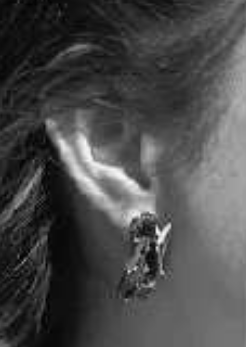
\includegraphics[width=.7\linewidth, height=5cm]{Imagenes/w1}
     \caption{Pendiente que mide la presión de la sangre}
     \label{fig:w1}
   \end{minipage}\hfill
   \begin {minipage}{0.48\textwidth}
     \centering
     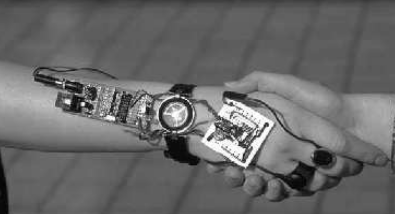
\includegraphics[width=.7\linewidth, height=5cm]{Imagenes/w2}
     \caption{Sensores y placa ajustados al brazo de una persona}
     \label{fig:w2}
   \end{minipage}
\end{figure}

\begin{figure}[]
   \begin{minipage}{0.48\textwidth}
     \centering
     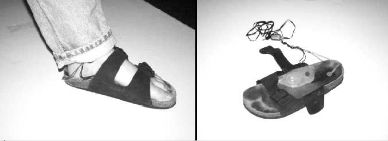
\includegraphics[width=.7\linewidth, height=5cm]{Imagenes/w3}
     \caption{Zapato utilizado para medir la conductancia de la piel}
     \label{fig:w3}
   \end{minipage}\hfill
   \begin {minipage}{0.48\textwidth}
     \centering
     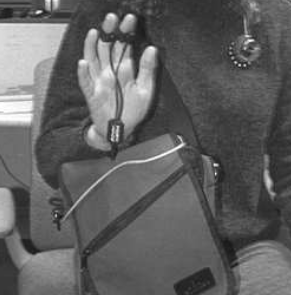
\includegraphics[width=.7\linewidth, height=5cm]{Imagenes/w4}
     \caption{Cámara digital, ordenador \textit{wearable} y sensores de la conductancia de la piel}
     \label{fig:w4}
   \end{minipage}
\end{figure}

\begin{figure}[]
   \begin{minipage}{0.48\textwidth}
     \centering
     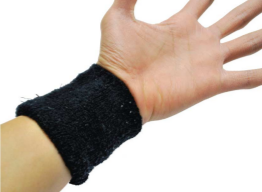
\includegraphics[width=.7\linewidth, height=5cm]{Imagenes/w5}
     \caption{Muñequera que mide la actividad electrodérmica de la piel}
     \label{fig:w5}
   \end{minipage}\hfill
   \begin {minipage}{0.48\textwidth}
     \centering
     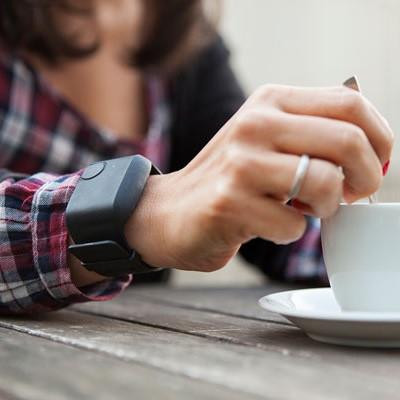
\includegraphics[width=.7\linewidth, height=5cm]{Imagenes/w6}
     \caption{Wristband de Empatica E4 que mide numerosas señales fisiológicas}
     \label{fig:w6}
   \end{minipage}
\end{figure}

\begin{figure}[]
   \begin{minipage}{0.48\textwidth}
     \centering
     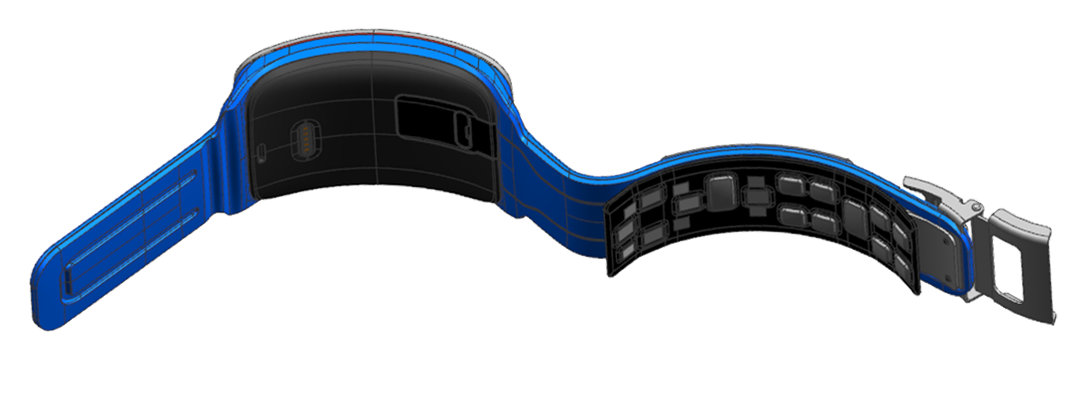
\includegraphics[width=.7\linewidth, height=5cm]{Imagenes/w7}
    \caption{Samsung Simband que mide numerosas señales fisiológicas}
     \label{fig:w7}
   \end{minipage}\hfill
   \begin {minipage}{0.48\textwidth}
     \centering
     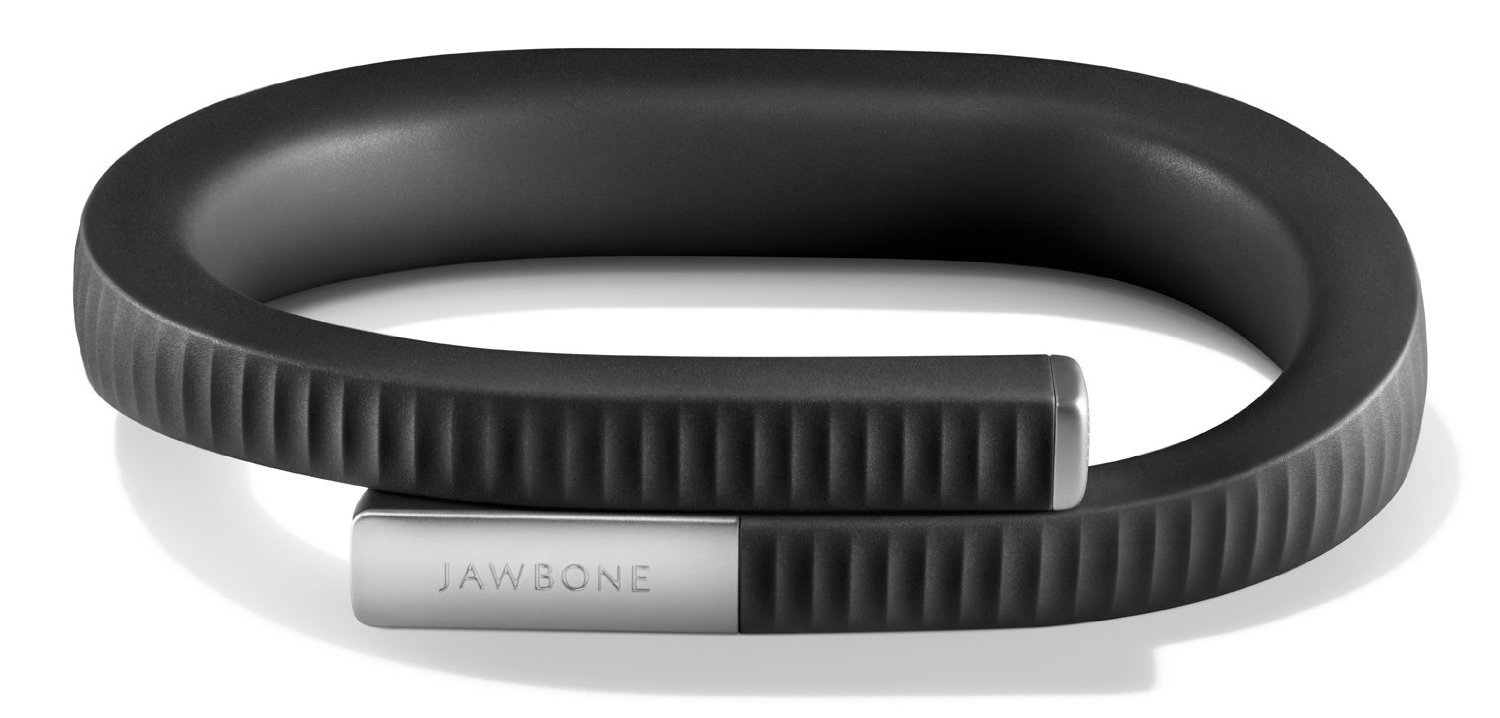
\includegraphics[width=.7\linewidth, height=5cm]{Imagenes/w8}
     \caption{Jawbone UP 24 que se utiliza para mejorar el rendimiento deportivo}
     \label{fig:w8}
   \end{minipage}
\end{figure}

%-------------------------------------------------------------------

\subsubsection{Pulseras inteligentes}
\label{subsubsec:pulserasInteligentes}
\paragraph{}
Actualmente existe una gran cantidad de pulseras inteligentes enfocadas a personas que quieran mejorar su rendimiento deportivo así como diversos estudios que comparan su fiabilidad \citep{sushames2016validity} \citep{baroni2015fitbit} \citep{kooiman2015reliability}. En esta sección se ha optado sin embargo por no saturar los ejemplos de las pulseras inteligentes de este último tipo puesto que es un enfoque que se aleja bastante del desarrollo de este trabajo. A continuación, se van a describir las características principales de una serie de pulseras inteligentes que sirven para medir distintas variables fisiológicas:

\begin{itemize}
    \item Fitbit Flex (\citeyear{martinez2015wristband}).
    \begin{itemize}
        \item Señales sensorizadas: ACC, HR.
        \item Objetivo: monitorización del sueño y de la actividad física.
        \item Fiabilidad: en un estudio que medía la monitorización del sueño con 107 sujetos realizada a lo largo de 7 días, el 86\% de los dispositivos no reconoció el sueño en 4 de estos 7 días y el 35\% de los dispositivos fue incapaz de reconocer el sueño en los 7 días del experimento\citep{baroni2015fitbit}. Otro estudio que medía la fiabilidad del contador del pasos con 48 muestras constataba que su validez es moderada, pues llegaba a tener margenes de error en el conteo de pasos de en torno al 20\%\citep{sushames2016validity}. Sin embargo, en una versión posterior llamada Fitbit Zip, esta pulsera fue la que obtuvo el menor margen de error entre otras 9 pulseras inteligentes en lo que respecta al conteo de pasos\citep{kooiman2015reliability}.
        \item Precio: actualmente está descatalogado. En el 2015 su precio era de 81€. Sus versiones posteriores cuestan en su tienda oficial entre 60 y 200€.
    \end{itemize}

    \item Jawbone UP 24 (\citeyear{jawbone24}).
    \begin{itemize}
        \item Señales sensorizadas: no especificadas en su documentación. A través de su API no es posible acceder a los datos sensorizados. Únicamente se pueden obtener datos procesados como los momentos en los que el usuario ha estado durmiendo.
        \item Objetivo: monitoreo de actividad física, del sueño y entrenador personal que aconseja al usuario para que tome decisiones saludables.
        \item Fiabilidad: según Tudor-Locke, los monitores de actividad no deberían sobrepasar un error del 1\% respecto a las mediciones del estándar de oro (en este caso respecto a las mediciones de pasos de Optogait\citeyear{optogait} en el laboratorio) para una prueba de conteo de pasos en una cinta mecánica a 4.8km/h para ser considerados fiables \citep{tudor2011many}. Siguiendo este mismo estándar, Jawbone UP es fiable según el estudio de Kooiman (\citeyear{kooiman2015reliability}).
        \item Precio: 75€.
    \end{itemize}

    \item Samsung Simband (\citeyear{simband}).
    \begin{itemize}
        \item Señales sensorizadas: ECG, PPG, ACC, ICG, EDA, SKT.
        \item Objetivo: monitoreo de señales fisiológicas.
        \item Fiabilidad: no se ha encontrado ningún estudio independiente que evalúe este producto.
        \item Precio: actualmente (2018) es gratuita para los investigadores tras rellenar una solicitud. Sin embargo, estas no siempre son aceptadas.
    \end{itemize}

    \item Empatica E4 (\citeyear{garbarino2014empatica}).
    \begin{itemize}
        \item Señales sensorizadas: EDA, PPG, SKT, HR, ACC.
        \item Objetivo: monitoreo de señales fisiológicas.
        \item Fiabilidad: a partir de un experimento con 7 sujetos, se exportó las señales ECG y PPG tanto con esta pulsera como con el estándar de oro con el que se comparó su fiabilidad, SEER Light Extend Recorder de General Electric. Las señales obtenidas fueron luego evaluadas por expertos y estudiantes de biomedicina, que evaluaban si la señal que observaban era real o no. El resultado obtenido fue que en el 85\% de los casos, ambos aparatos devolvieron datos con calidad similar, obteniendo datos de mejor calidad con el sensor de General Electric en un 5\% de los casos \citep{mccarthy2016validation}.
        \item Precio: 1372€.
    \end{itemize}

    \item Dispositivo: MoodMetric (\citeyear{moodmetric}).
    \begin{itemize}
        \item Señales sensorizadas: EDA.
        \item Objetivo: monitoreo de señales fisiológicas.
        \item Fiabilidad: en un estudio del instituto finés de ocupación para la salud con 24 voluntarios de entre 19 a 31 años se compararon las señales sensorizadas de EDA del prototipo de este anillo con un aparato de laboratorio para medir esa misma señal fisiológica, SA9309M. El resultado obtenido fue de una similaridad de la señal entre ambos dispositivos en un 83 y 16,4\% de los casos, concluyendo que dicho protitipo \textit{es un dispositivo prometedor para estudios ecológicamente válidos} \citep{torniainen2015feasibility}.
        \item Precio: 1.372€.
    \end{itemize}

\end{itemize}

\subsubsection{Comparativa de pulseras inteligentes}
\label{subsubsec:comparativaPulseras}
\paragraph{}
En la tabla~\ref{tab:accesoriosComparativa} se muestra una comparativa de los accesorios inteligentes citados en la sección anterior en base a la caracterización fisiológica de la ira descrita en la sección~\ref{subsubsec:fisioIra}. Como se puede ver en la tabla~\ref{tab:accesoriosComparativa}, se han descartado cinco de las trece características de la ira puesto que estas no se pueden medir con pulseras o anillos inteligentes al hacer referencia a variaciones de partes del cuerpo que no incluyen a los dedos de las manos o las muñecas (es el caso de la temperatura periférica facial) o ser referencias a sensaciones subjetivas que no se pueden discretizar de manera directa mediante pulseras o anillos inteligentes (es el caso de la sensación de desmayo, los sudores fríos, dolor de estómago y náuseas).

\paragraph{}
Como se puede ver en la tabla~\ref{tab:accesoriosComparativa}, los dos accesorios inteligentes que miden más señales fisiológicas de la ira son Samsung Simband y Empatica E4. Existen otra serie de elementos que pueden ayudar a seleccionar la mejor de las opciones entre ambas, como puede ser el precio, el tamaño y actividad de las comunidades de desarrolladores que utilizan estos productos o la versatilidad de sus \ac{SDK}. [TODO: según la solución que finalmente se elija, completar este párrafo de una u otra manera]

\paragraph{}
Respecto a las otras opciones comparadas, Jawbone UP 24 no está diseñada para ser utilizada por investigadores pues ni siquiera provee la caracterización de los sensores utilizados (de ahí que no haya sido posible cumplimentar la tabla para este accesorio inteligente). Fitbit Flex puede sensorizar la tasa cardíaca y los temblores a partir de su acelerómetro. Este accesorio, sin embargo, incluso en el caso de que pudiese sensorizar más información que el resto de accesorios debería ser descartada por sus grandes fallas de medición, tal y como se comentó en la sección~\ref{subsubsec:pulserasInteligentes}. Por último, el anillo de Moodmetric tiene el problema de ser excesivamente limitado, pues sólo es capaz de medir la actividad electrodérmica de la piel.

[TODO: según la solución que finalmente se elija, completar con un párrafo adicional de una u otra manera]


\begin{landscape}
\thispagestyle{plain}
\begin{table}[]
\centering
\caption{Comparativa de accesorios inteligentes para la medición de la ira}
\label{tab:accesoriosComparativa}
\begin{tabular}{|c|c|c|c|c|c|c|c|c|}
\hline
                                            & \textbf{\begin{tabular}[c]{@{}c@{}}Presión\\ arterial\end{tabular}} & \textbf{\begin{tabular}[c]{@{}c@{}}Tasa\\ cardíaca\end{tabular}} & \textbf{\begin{tabular}[c]{@{}c@{}}Tasa\\ respiratoria\end{tabular}} & \textbf{Temblores} & \textbf{\begin{tabular}[c]{@{}c@{}}Enrojecimiento\\ de la piel\end{tabular}} & \textbf{\begin{tabular}[c]{@{}c@{}}Tensión\\ muscular\end{tabular}} & \textbf{\begin{tabular}[c]{@{}c@{}}Sudor en\\ las manos\end{tabular}} & \textbf{\begin{tabular}[c]{@{}c@{}}Coductividad\\ de la piel\end{tabular}} \\ \hline
\textbf{Fitbit Flex}                                               & \xmark                                                                  & \cmark                                                               & \xmark                                                                   & \cmark                 & \xmark                                                                           & \xmark                                                                  & \xmark                                                                    & \xmark                                                                         \\ \hline
\textbf{Empatia E4}                                                & \cmark                                                                  & \cmark                                                               & \xmark                                                                   & \cmark                 & \xmark                                                                           & \xmark                                                                  & \xmark                                                                    & \cmark                                                                         \\ \hline
\textbf{MoodMetric}                                                & \xmark                                                                  & \xmark                                                               & \xmark                                                                   & \xmark                 & \xmark                                                                           & \xmark                                                                  & \xmark                                                                    & \cmark                                                                         \\ \hline
\end{tabular}
\end{table}
\end{landscape}

%-------------------------------------------------------------------

\section{Código deontológico}
\label{section:codDeonto}

\subparagraph{}
Puesto que en este proyecto se va a realizar una evaluación con seres humanos, es necesario conocer el código deontológico utilizado en psicología con el fin de evitar malas prácticas. Para este proyecto, se ha seguido el código deontológico utilizado por el Consejo General de Colegios Oficiales de Psicólogos de España en su versión aprobada el 6 de marzo de 2010 (a pesar de realizar este trabajo como informático y por tanto no estar regido por dicho código deontológico, se considera imprescindible asumir de propia iniciativa dicho código deontológico). Los principales postulados que afectan directamente a la investigación de este proyecto son los siguientes:
\begin{itemize}
    \item Finalidad humana y social de la psicología.
    \item Respeto a la persona y protección de los derechos humanos.
    \item No realización de prácticas que atenten contra la libertad e integridad psíquica y física de las personas.
    \item Utilización cautelar del lenguaje con el fin de evitar etiquetas devaluadoras y discriminatorias.
    \item Asegurar la libertad de los sujetos a la hora de formar parte del experimento.
    \item Respeto de la intimidad de los sujetos conjugada a través de la no divulgación de los datos obtenidos sin que estos hayan sido previamente anonimizados.
\end{itemize}
\cleardoublepage % Empty page before the start of the next part
%---------------------------------------------------------------------
%
%                          Capítulo 2 - Herramientas tecnológicas
%
%---------------------------------------------------------------------

\chapter{Herramientas tecnológicas}

\paragraph{}
En este capítulo, se van a explicar las distintas opciones tecnológicas que se han barajado a la hora de realizar este trabajo hasta llegar a la solución final. Las decisiones clave han sido el tipo de base de datos para guardar los registros generados durante las interacciones entre dispositivos (sección ~\ref{sec:tipoBD}), la elección de protocolos de comunicación de los datos (sección ~\ref{sec:protoCom}),  y los protocolos de ciberseguridad (sección ~\ref{sec:ciber}.


%-------------------------------------------------------------------
\section{Lenguaje de programación de la aplicación web}
\paragraph{}
Para el lenguaje de programación de la aplicación web se barajaban dos opciones: Java y Python. En este caso, el único motivo por el que se utilizó Python en lugar de Java fue simplemente porque se contaba con experiencia previa desarrollando aplicaciones web con ambos lenguajes y había resultado bastante más fácil e intuitivo el desarrollo web con Python. Así, sin necesidad de utilizar variables externas, se decidió que \textbf{el lenguaje de programación utilizado para desarrollar la aplicación web sería Python, concretamente usando el \textit{framework} de Flask}.

\section{Sistema operativo para la aplicación móvil}
\paragraph{}
A la hora de elegir el sistema operativo objetivo para la aplicación móvil, hay un elemento fundamental que se debe tener en cuenta: la cuota de mercado de cada uno de ellos. Así, en una encuesta de 2019 de StatCounter~\citep{statCounter} se podía ver que el 74,45\% de la cuota global de usuarios móviles utilizaban Android, frente al 22,85\% que usan iOS y un 2,7\% que utilizan otros sistemas operativos. Sumando esto al hecho de que existe una comunidad de desarrolladores Android mucho más activa que la de iOS y que no se contaba con ningún dispositivo iOS para poder realizar el desarrollo, \textbf{se optó por programar una aplicación móvil para Android}.

\section{Interfaz web}
\paragraph{}
Para el diseño de la interfaz de la página web, las dos opciones que se barajaron fueron Bootstrap y Bulma. Las principales ventajas de Bootstrap son que tiene una comunidad de desarrolladores mucho más activa que Bulma, es una solución con una cuota de mercado bastante superior, lo que hace que tengan una gama mucho mayor de componentes que se puedan añadir a la web. Las principales desventajas respecto a Bulma son que es más complicado de aprender y no existe gran flexibilidad en cuanto a la modificación de sus componentes. Hay otro elemento adicional que dependiendo del caso puede ser una ventaja o una desventaja que es que Bulma es únicamente un paquete de CSS mientras que Bootstrap incorpora Javascript. Para este proyecto, ambas soluciones son perfectamente válidas, pero \textbf{la solución que se ha implementado ha sido con Bulma}, ya que este es un proyecto mediano, sin gran complejidad en el diseño, en el que la estructura basada en cajas encaja a la perfección con este framework.

\section{Bases de datos}
\label{sec:tipoBD}
\paragraph{}
Las bases de datos son conjuntos de información almacenadas con un determinado orden para facilitar su manipulación. Los dos tipos principales de bases de datos son:

\begin{itemize}

\item Bases de datos relacionales: aquellas que siguen el modelo de la lógica de predicados y se utilizan generalmente para almacenar lo que se denominan datos \textit{clásicos}. Es decir, se suelen usar cuando se espera que el resultado de una consulta sea una tupla de valores con la forma exacta con la que se han solicitado, eliminando así la incertidumbre respecto a la definición de las columnas de los elementos que se encuentran en la base de datos \citep{jimenez2016implementacion}. Estas bases de datos a su vez deben de tener definidas al menos las reglas de inserción, actualización y eliminación de datos \citep{codd1979extending}. La principal desventaja de las bases de datos relacionales es su baja escalabilidad debido a que fueron diseñadas para alojar los datos en un único servidor con el fin de garantizar la integridad del mapeado de las tablas así como evitar los problemas de la computación distribuida, como podría ser en este caso la modificación de un dato replicado en varios servidores. A esto se le añade la dificultad para lidiar con datos que no tengan una estructura previamente conocida y/o fuertemente tipificada. Por otro lado, existe una gran comunidad de desarrolladores utilizando bases de datos relacionales como SQL lo que facilita su implementación. Estas bases de datos pueden ser muy útiles, por ejemplo, para almacenar los datos de registro de usuarios en una página web en la que existen una serie de campos estándar que se pretenden mantener sin grandes modificaciones a lo largo del tiempo.

\item Bases de datos no relacionales: se basan en una mayor flexibilidad a la hora de almacenar datos con atributos y contenido dispar, pudiendo añadir nuevos atributos sin tener que modificar el contenido de otros registros. Estas bases de datos suelen facilitar la escalabilidad horizontal así como la posibilidad de replicar y distribuir los datos entre los distintos servidores, al poderse particionar los datos por patrones. Un ejemplo de caso de uso de este tipo de bases de datos es el almacenamiento de sensorizaciones de una instalación en la que pueda haber un número indeterminado de tipos de datos que puedan llegar en cada momento, así como que estos, dependiendo de la marca de los dispositivos instalados, puedan estar etiquetados de distinta manera. Entre las bases de datos no relaciones o no-sql podemos encontrar los siguientes tipos \citep{aws-nosql}:
\begin{itemize}
\item Clave-valor: son altamente divisibles y permiten un gran escalado horizontal. Algunos de sus casos de uso son los videojuegos, la tecnología publicitaria o IOT. Algunos ejemplos de estas bases de datos son Redis y Cassandra.
\item Documento: es un modelo que no se basa en filas y columnas desnormalizadas, sino que los datos se presentan en formatos como JSON. Algunos ejemplos de estas bases de datos son MongoDB y CouchDB.
\item Gráficas: son principalmente usadas en aplicaciones que trabajan con conjuntos de datos fuertemente conectados, como es el caso de los datos relacionados con las redes sociales, motores de recomendaciones y gráficos de conocimiento. Entre este tipo de base de datos se encuentran Neo4j y OrientDB.
\end{itemize}

\paragraph{}
En el caso de las bases de datos no relaciones, la diferencia entre las distintas soluciones tecnológicas es bastante significativa. Algunos de los factores a tener en cuenta a la hora de decantarse por algunas de estas tecnologías son:

\begin{enumerate}
\item La bases de datos pueden tener licencias tanto privativas como de software libre. Si se elige una solución de software libre no habrá limitaciones en el conocimiento que se puede tener sobre la tecnología en cuestión.
\item La interacción con la base de datos. Esta facilidad es subjetiva y no es el propósito de este trabajo buscar métodos que estandaricen dicha medición entre distintos perfiles de programadores. Por tanto, este punto debe ser considerado en función del equipo que vaya a trabajar con la base de datos elegida.
\item Fácil interacción en el medio tecnológico en el que se vaya a interactuar con la base de datos (un ordenador, un Arduino, un móvil, etc).
\item Debe poseer una comunidad de desarrolladores que facilite la resolución de dudas. Esto puede verse reflejado principalmente en los índices de popularidad de los lenguajes en foros de programación como Stackoverflow.
\item Debe disponer de una versión estable.
\item Persistencia de la base de datos. Si se quieren guardar los datos históricos de una aplicación, será necesario que esta base de datos sea persistente.
\end{enumerate}

\paragraph{}
Teniendo como referencia la facilidad del programador de este proyecto con las distintas bases de datos (punto 2), las opciones que se barajan son Cassandra, MongoDB y Couchbase. Estas soluciones teconológicos son todas ellas de software libre (punto 1), con una fácil interaccion en Python y Java (punto 3), que son los dos lenguajes de programación que se barajan en este proyecto y todos ellos llevan por lo menos siete años siendo públicos, por lo que se considera que cumplen también el punto 5.

\paragraph{}
En el caso de Cassandra, a pesar de encontrarse entre las quince bases de datos más utilizadas según la encuesta de Stackoverflow de 2018 \citep{so-db}, ni siquiera en la propia documentación de las páginas oficiales de estos lenguajes se explica cómo interactuar con Android. Por otro lado, Couchbase y MongoDB  cuentan con documentación para Android en sus respectivas páginas oficiales así como proyectos de ejemplo en los que queda bastante claro la manera de interactuar con las bases de datos. En el caso de Couchbase, esta cuenta con un sistema de consultas de datos llamado N1QL que intenta servir como puente entre el formato de consultas con sintaxis más farragosas como las de Mongo y las sentencias de bases de dato SQL.

\paragraph{}
Por último, tanto MongoDB como Couchbase cuentan con contenedores Docker ya configurados así como tutoriales que facilitan su puesta en marcha y modificación. Ambas cuentan con una comunidad activa de de desarrolladores, pero MongoDB actualmente (2019) es una tecnología bastante más popular que Couchbase.
\end{itemize}

\paragraph{}
En este trabajo, \textbf{se ha decidido usar MongoDB para almacenar la información del servidor} ya que es una base de datos con una sintaxis sencilla, con librería específica en Python, es ideal para soluciones distribuidas y es una base de datos no relacional, lo que facilitará el almacenamiento de datos con estructuras variables. Estas características se ajustan a posibles actualizaciones futuras de las estructuras de la base de datos sin tener que migrar todos los registros que ya están almacenados. Por ejemplo, si se permitiese en el futuro que el paciente pudiese subir una fotografía para identificarse, el token identificador de esta fotografía se podría añadir para los nuevos pacientes en la misma colección que la del resto de registros de pacientes antiguos sin fotografías. Por último, el flujo de datos de episodios puede ser muy elevado a largo plazo, por lo que una solución distribuida como es el caso de MongoDB facilitará la escalabilidad de la base de datos.

\paragraph{}
Por otro lado, a la hora de elegir el sistema de bases de datos para la aplicación Android, existe un abanico mucho más acotado de opciones. Existen alternativas no relacionales para Android como Couchbase o WaspDB, aunque en esta categoría sin duda destaca la solución tecnológica de Google, Firebase. Con este tipo de base de datos se cuenta con un poco de experiencia en proyectos previos, en donde se veía que no encajaría del todo para este proyecto puesto que está más enfocado en el streaming de datos así como en el uso de los servidores de Google para dicha gestión, lo que restringe la posibilidad de poder tener los datos en un servidor propio sobre el que se tenga el completo control.

\paragraph{}
Dadas estas circunstancias, se decidió usar SQLite como base de datos local para la aplicación Android, que es un estándar en el desarrollo de aplicaciones móviles. Como complemento, Android cuenta con un tipo de base de datos con formato clave-valor llamado \textit{sharepreferences}. Este tipo de base de datos es útil cuando las consultas y operaciones que se quiere realizar sobre los datos son sencillas. Así, \textbf{se ha decidido usar SQLite para almacenar información compleja} como las pautas y los episodios de ira \textbf{y \textit{sharepreferences} para información con menor nivel de complejidad}, como almacenar el último nivel de ira o los segundos que lleva un usuario desde su último episodio de ira.

\section{Protocolos de comunicación}
\label{sec:protoCom}
\paragraph{}
Los datos sensorizados por la pulsera electrónica deben de ser enviados periódicamente al servidor para poder ser analizados por el terapeuta. Estos datos son alfanuméricos y no es necesario disponer de ellos en el servidor tan pronto como sean generados, puesto que cuando van a ser revisados por el terapeuta es antes de la consulta para preparar la terapia y durante la misma para ratificar la información almacenada del paciente. Es importante que la aplicación no requiera de un elevado coste de uso de red ni consuma excesiva batería del móvil, pues se espera que la aplicación no sea intensiva en el uso de recursos para que por un lado pueda ser usado en una mayor gama de teléfonos móviles y por otro no suponga una molestia al usuario que termine con la desactivación de la aplicación. Esto se debe a que los teléfonos móviles inteligentes actualmente se utilizan para un abanico muy amplio de tareas que van más allá de las llamadas telefónicas, por lo que, al crecer con los años la dependencia de las personas en estos dispositivos, es importante que la aplicación no interfiera gravemente con los otros usos que se le vaya a dar al dispositivo.

\paragraph{}
Los protocolos de comunicación que se van a analizar van a depender en cada caso de las características de los dispostivos que se comunican así como de la ciberseguridad necesaria para entablar dicha comunicación. A conti-\\nuación se van a detallar los tipos de comunicaciones que son necesarias en el proyecto con las distintas implementaciones posibles.

\subsection{Comunicación entre el móvil Android y la pulsera}
\paragraph{}
La característica más importante que debe tener el protocolo utilizado es que debe ser de muy bajo consumo para maximizar la duración de la batería de la pulsera inteligente. A su vez, esta comunicación está limitada por los protocolos válidos entre los distintos modelos de móviles y de pulseras. Por este motivo, \textbf{la opción que se ha escogido es utilizar el protocolo BLE}, puesto que es compatible con la gran mayoría de dispositivos móviles inteligente así como de las pulseras inteligentes, lo que hace que la solución no quede anclada a ningún elemento físico. Este protocolo, como su propio nombre indica, es un protocolo de bajo consumo lo que reducirá el consumo eléctrico respecto a otros protocolos como Bluetooth 2.0.

\subsection{Comunicación entre el dispositivo móvil Android y el servidor}
\label{subsec:comAndroidServ}
\paragraph{}
Una vez han llegado los datos de las sensorizaciones al móvil, estos datos se envían al servidor. Este envío se puede realizar mediante peticiones Hypertext Transfer Protocol(HTTP), Message Queuing Telemetry Transport (MQTT) o Advanced Message Queuing Protocol (AMQP).

\paragraph{}
La principal diferencia entre las peticiones HTTP y las peticiones MQTT Y AMQP es el consumo de recursos de estas soluciones, siendo MQTT un protocolo más eficiente en el envío de paquetes que HTTP \citep{yokotani2016comparison}, que es un elemento crítico en IOT, puesto que los dispositivos IOT no suelen estar conectados a la corriente continua, lo que hace que el consumo de energía de los dispositivos IOT sea un factor crucial a la hora de tomar decisiones tecnológicas. Por este motivo, el protocolo HTTP queda descartado.

\paragraph{}
El protocolo MQTT es un protocolo unidireccional entre un publicador y un suscriptor a través de unos identificadores del canal llamado tópicos. En lo que respecta a asegurar que los datos del publicador han llegado al suscriptor, existen tres niveles de Quality of Service (QoS) que se pueden definir por cada tópico. En el nivel cero, se envía el dato al menos una vez pero no se garantiza que ese dato ha llegado al suscriptor. En el nivel uno, el suscriptor debe enviar la confirmación de que le ha llegado el dato en cuestión al menos una vez. Por último, en el nivel dos, se garantiza que el dato llega exactamente una vez al suscriptor.

\paragraph{}
AMQP se diferencia principalmente de MQTT en que en AMQP el servidor puede mandar mensajes de vuelta al cliente que vayan más allá de los mensajes numéricos de posibles errores. Esto tiene como coste un mayor consumo de ancho de banda, pero mucho menor que en el caso de HTTP. En el caso de MQTT si se quiere establecer esta comunicación bidireccional es necesario crear dos canales entre ambos elementos.

\paragraph{}
En lo que respecta a la autenticación y la ciberseguridad, ambos protocolos pueden ser integrados con TLS. El ancho de banda de esta solución en MQTT únicamente se ve notablemente resentida en la etapa de autenticación, mientras que en las fases posteriores de envío de datos el rendimiento es muy similar a las soluciones sin TLS \citep{hivemq}.

\paragraph{}
En este trabajo inicialmente se decidió usar el protocolo AMQP ya que en su implementación de RabbitMQ permite una fácil integración en múltiples lenguajes, pero tras realizar varias pruebas fue descartado ya que tanto MQTT como AMQP se basan en la utilización de unas colas de mensajes que pueden ser problemáticas en el caso de que el servidor estuviese caído o la petición fuese incorrecta, ya que se comprobó que esto hacía necesario el vaciamiento a mano de la cola de mensajes. Esto no ocurre con las peticiones Rest, que son procesos ácidos en los que en caso de que el servidor esté caído o que la URL o los datos sean incorrectos, o bien simplemente la petición no llegará a su destino y se volverá a enviar después o llegará a su destino y con detectores de errores bastante sencillos se evitará que la aplicación quede estancada por una petición incorrecta. Esto como digo se comprobó que con AMQP era bastante más complejo de gestionar, por lo que \textbf{se ha optado por utilizar API REST para la comunicación entre la aplicación Android y el servidor}, a pesar de que como se ha comentado, las peticiones HTTP suponen un mayor consumo de datos que las peticiones AMQP.

\section{Ciberseguridad}
\label{sec:ciber}
\paragraph{}
Como se va a tratar con datos biométricos sensibles, es importante asegurarse de que esta información no acabe en manos indeseadas. Con este fin, es importante tomar las siguientes medidas de seguridad:
\begin{enumerate}
\item Autenticación tanto en la base de datos del móvil como en la base de datos del servidor. En el caso de la base de datos del servidor, no se debe permitir las conexiones externas que trabajen directamente con la base de datos.
\item Encriptación de los datos de ambas bases de datos, para que aunque un atacante consiguiese tener acceso al dispositivo, no pudiese obtener información de la propia base de datos.
\item Encriptación punto a punto, para evitar ataques de \textit{sniffing}.
\end{enumerate}

\paragraph{}
El punto más vulnerable de la solución será el envío de datos de la pulsera al dispositivo Android, pues este envío viene configurado por el propio desarrollador de la pulsera y se realiza sin ningún tipo de cifrado, por lo que si un atacante se hace con el control del dispositivo Android, podrá leer directamente los datos que son enviados por BLE sin tener que forzar ni nuestra app ni nuestras bases de datos.

\paragraph{}
El servidor web debería requerir que los usuarios se autentiquen antes de poder operar con los datos de las mediciones para evitar accesos indeseados a la base de datos con los registros de sensorizaciones. A continuación se van a describir distintos métodos de autenticación que se pueden implementar.

\begin{itemize}
\item Autenticación básica: el usuario se identifica mediante una tupla usuario-contraseña que son enviados en texto plano. Esto tiene numerosas vulnerabilidades, como la escucha de terceros así como el hecho de que al no contar con claves API que funcionen por debajo de la contraseña del usuario, se impide que el responsable de la seguridad del servidor pueda cambiar las claves API en caso de detectar alguna posible vulnerabilidad. Por contra, en este caso por cada cambio que se realice se requiere la interacción del usuario.

\item OAuth 1.0: es un protocolo basado en la autorización en lugar de la autenticación en la que los consumidores y los proveedores no intercambian las claves de acceso sino claves que autorizan al consumidor para realizar determinadas operaciones. Es un modelo similar al de las claves de coches de lujo de tipo valet, que permiten acceder sólo a recursos concretos del coche (por ejemplo, con estas llaves se puede conducir el coche pero no utilizar el ordenador de abordo) y sólo durante un periodo de uso concreto (por ejemplo, la llave deja de funcionar si se sobrepasan los 10 kilómetros de autonomía que se establecen para que un chófer pueda aparcar dicho coche pero no pueda utilizarlo para dar una vuelta), en contraposición de la llave del coche tradicional que autoriza para realizar cualquier operación sin que esta llave nunca caduque \citep{oauth1}. Los tres actores que intervienen en este protocolo son el usuario, el consumidor y el proveedor del servicio. A continuación se van a desgranar a partir del artículo de Rob Sobers (\citeyear{robsobers}) el flujo que sigue un usuario cuando accede correctamente a un recurso protegido:
\begin{enumerate}
\item El usuario muestra su intención de acceder a un determinado recurso.
\item El consumidor pregunta al proveedor del servicio si puede darle permiso al usuario. El proveedor de servicio provee al consumidor un token y un secreto para acceder al recurso.
\item El consumidor le envía al usuario este token y su correspondiente secreto. 
\item El usuario le envía al proveedor del servicio una solicitud para que autorice el token que le ha enviado el consumidor, respondiendo si dicho token es correcto.
\item El consumidor cambia con el proveedor del servicio el token de solicitud obtenido en el paso 2 por un token de acceso.
\item El consumidor accede al recurso protegido con su token.
\end{enumerate}

\item OAuth 2.0: como su nombre indica, es la segunda versión del protocolo Oauth 1.0, que aumenta significativamente su usabilidad. Las principales diferencias de OAuth 2.0 frente a OAuth 1.0 son las siguientes \citep{oauth2}:
\begin{itemize}
\item Mejor experiencia de usuario para accesos desde dispositivos móviles: para usar OAuth 1.0 en las apps, era necesario redirigir al usuario al navegador, que este introdujese ahí sus credenciales, en caso de que fueran correctos copiar el token de autorización e introducirlo de vuelta en la app. En OAuth 2.0 este proceso se puede realizar sin tener que salir de la propia app.
\item Simplificación de las firmas: ya no hace falta una codificación con-\\ creta y utiliza un único secreto en lugar de dos.
\item Se incluye la posibilidad de incluir tokens de actualización. Estos son tokens que se envían junto a los credenciales del usuario cuando el token de acceso ha caducado para solicitar un nuevo token. Este token por tanto, no tiene ninguna utilidad si no se tienen a su vez los credenciales de acceso.
\item Separación clara de roles entre el servidor que responde a las solicitudes de OAuth y los servidores encargados de la autenticación del usuario.
\end{itemize}

\item JWT (Json Web Token authentification): es un método que utiliza un objeto JSON para autentificar usuarios o enviar información de forma segura. La información que se manda puede ser firmada con HMAC-SHA256, o con RSA o ECDSA \citep{jwt}. El objeto JSON que se envía tiene la siguiente estructura \citep{rfc7519}:
\begin{itemize}
    \item Cabecera: es donde se define el algoritmo utilizado para realizar la firma (HMAC, RSA o ECDSA).
    \item Carga útil o \textit{payload}: es donde se realiza la petición que debe ser contrastada. Existen tres tipos de peticiones:
    \begin{itemize}
        \item Peticiones registradas: son una serie de peticiones predefinidas que se recomienda usar. Entre ellas, se encuentra \texttt{iss}, que identifica al emisor del JSON o \texttt{exp}, que establece el momento en el que el JSON deja de ser válido.
        \item Peticiones públicas: es una lista de peticiones más extensa que las registradas en las que por ejemplo se puede definir el correo electrónico, la zona horaria o la localización del emisor, tal como se puede consultar en la página web de IANA \citeyear{iana}.
        \item Peticiones privadas: son peticiones personalizadas que el productor y consumidor del objeto JWT previamente han decidido usar.
    \end{itemize}
    \item Firma: se incluye la firma de la cabecera y de la carga útil.
\end{itemize}

\item TLS (Transport Layer Security)/SSL(Secure Socket Layer): son dos protocolos de critografía asimétrica que se suelen utilizar indistintamente y que se usan para establecer comunicaciones seguras en la red. TLS contiene dos capas: la capa para el apretón de manos, en la que autentifica a ambas partes, y la capa en la que se provee seguridad en cuanto a la integridad del mensaje \citep{evaldsson2015evaluate}. Una de sus principales fortalezas es la interoperabilidad: no se impone un método de encriptación entre el cliente y el servidor, sino que se negocia dicho método entre ambos, lo que permite renovar viejos protocolos de encriptación cuando estos quedan obsoletos \citep{carlsson2018comparison}. Su aplicación más conocida es para establecer comunicaciones seguras entre el servidor y el navegador web al realizar peticiones HTTP. Entre estos dos protocolos, SSL es el protocolo de seguridad más utilizado para la autenticación en Internet \citep{viega2002network}.
\end{itemize}

\paragraph{}
\textbf{Se ha decidido usar el protocolo de ciberseguridad TLS}, ya que esta es la solución más extendida de todas las comentadas y tiene soporte e integración directa con AMQP, el protocolo de comunicación que se va a utilizar para conectar el móvil y la pulsera, tal y como se indicó en el apartado~\ref{subsec:comAndroidServ}.
\cleardoublepage % Empty page before the start of the next part
%---------------------------------------------------------------------
%
%                          Capítulo 4 - Descripción del problema
%
%---------------------------------------------------------------------

\chapter{Termómetro de la ira}

En este capítulo se va a detallar el proceso que se ha seguido para llegar a implementar el termómetro de la ira. En la sección~\ref{sec:c4:intro} se introduce el problema al que se desea dar solución con el termómetro de la ira. En la sección~\ref{sec:c4:cap} se explica cómo se ha llevado a cabo la captura de requisitos y cuáles fueron los requisitos iniciales de la aplicación. En la sección~\ref{sec:c4:diseño} se explica cómo se desarrolló el diseño de la aplicación con la ayuda de los usuarios finales y la experta en el tratamiento de la ira. Por último, en la sección~\ref{sec:c4:impl}, se detalla cómo se ha implementado y se muestra el resultado final.

%-------------------------------------------------------------------
\section{Introducción}
\label{sec:c4:intro}
\paragraph{}
A la hora de tratar clínicamente a un paciente con problemas de salud mental, existe el problema de que aquello que cuenta el paciente sobre su problema puede no corresponderse con la realidad. Un paciente puede acudir por voluntad propia o de terceros y tanto su versión como la interpretación de los hechos que le han llevado a la consulta pueden diferir severamente entre cada persona. En el caso concreto de la ira, tal y como se comentaba en la sección~\ref{subsubsec:intervencionPsico}, la ira se desarrolla en entornos muy específicos (y diferentes entre cada paciente), supone una distorsión intencionada de la realidad y, por la deseabilidad social del paciente, puede que niegue que tenga problemas de gestión de la ira a la hora de dirigirse al terapeuta.

\paragraph{}
Por todo ello, se propone una solución tecnológica en la que, por un lado el paciente pueda tener en tiempo real información que le sea de utilidad para gestionar dicho episodio de ir y, por otro, dé información adicional a la terapeuta para guiar la consulta para la gestión de la ira. Se propone un sistema tecnológico que mida de forma continuada las constantes fisiológicas del paciente sin que esto interfiera en su día a día, interprete y detecte los episodios de ira y cuando surja un episodio de ira, la aplicación le dará una serie de pautas (previamente cargadas en el sistema por el terapeuta) que le ayuden a gestionar el episodio de ira para volver a una situación de calma. Toda la información del paciente se irá registrando para su posterior análisis por parte del terapeuta. La información recogida resultará de gran ayuda para detectar si el tratamiento está siendo efectivo (es decir, si los episodios de ira disminuyen en intensidad, duración y frecuencia a lo largo del tiempo) y si las pautas asignadas por el terapeuta son o no efectivas.

\paragraph{}
Para medir las constantes fisiológicas se utilizará una pulsera inteligente, que es un formato de dispositivo inteligente ampliamente usado entre segmentos muy diversos de la población, lo que evitará la estigmatización del paciente ya que nadie tiene por qué saber el uso que se está dando a la pulsera.

\paragraph{}
Es importante recalcar que esta solución tecnológica bajo ningún concepto pretende sustituir la terapia con el paciente. Por contra, es una herramienta adicional que intenta mejorar los resultados de la atención clínica al paciente en cuestión.

\paragraph{}
Debido a que no somos expertos en el tratamieto de la ira, en este proceso será fundamental realizar un diseño centrado en el usuario, en el que se contará en todas las fases del proceso con una persona experta que trabaja con la gestión de la ira.

\section{Captura de requisitos}
\label{sec:c4:cap}
\paragraph{}
Una vez identificado el problema, es fundamental establecer contacto con usuarios finales de la aplicación para capturar los requisitos. En este caso, existen dos perfiles de usuarios finales: los pacientes con ira disfuncional y los terapeutas de dichos pacientes. Para este caso, se ha incorporado el conocimiento de una psicóloga que trabaja con este tipo de pacientes que guiará el diseño no solo en lo que concierne a la información que le será útil al terapeuta sino también a qué y cómo debe presentarse la información a los pacientes con ira disfuncional.

\paragraph{}
Para la captura de requisitos, se han realizado dos reuniones con la psicóloga en las que se han recogido unos requisitos que tengan en cuenta tanto las necesidades de los usuario finales como las restricciones tecnológicas. Así, los requisitos funcionales que se han definido tras estas reuniones son:

\begin{enumerate}
    \item Una pulsera inteligente recogerá las constantes fisiológicas a partir de las cuales se intentará averiguar si dicho paciente está sufriendo ira.
    \item El paciente tendrá una aplicación instalada en su móvil, cuyo sistema operativo debe ser Android.
    \item El terapeuta tendrá una aplicación web donde podrá ver el registro de episodios de sus pacientes así como modificar las pautas asociadas a cada uno de ellos.
    \item Cuando se detecte que el paciente pueda estar sufriendo ira, en el móvil del paciente, deberán aparecerle pautas que le ayuden a gestionar dicha ira hasta que se detecte que el episodio ha terminado (el paciente ha vuelto a un estado de calma).
    \item El grado de ira que se le presentará al paciente en un termómetro horizontal en el que el menor valor esté a la izquierda y el valor de mayor ira esté a la derecha.
    \item El paciente podrá descartar pautas y emitir comentarios sobre las mismas para así poder afinar mejor las pautas que les son útiles a cada paciente.
    \item Se registrará el uso y desuso de las pautas para cada paciente, pudiendo el terapeuta modificarlas convenientemente si viese que estas no están siendo útiles.
    \item Todos los episodios de ira del paciente serán registrados para su posterior revisión por parte del terapeuta y del propio paciente.
    \item Las pautas deben de ser definidas por el terapeuta.
    \item La aplicación móvil para el paciente debe ser muy visual y con una curva de aprendizaje poco elevada, lo que implicará limitar el rango de acciones disponibles para el usuario.
    \item Los textos de la aplicación deberán ser en lectura fácil\footnote{Los textos de lectura fácil son aquellos que se realizan con un vocabulario sencillo para que estos puedan ser comprendidos por personas con discapacidad intelectual.} para que estos puedan ser accesibles para todo tipo de usuarios.
\end{enumerate}

\section{Diseño}
\label{sec:c4:diseño}
\paragraph{}
Una vez establecidos los requisitos que debe cumplir la aplicación, se definió la interfaz y las interacciones. El diseño se ha creado en dos iteracciones que se presentan en detalle en las siguientes subsecciones. En la primera iteracción se utilizaron prototipos en papel porque es una solución que requiere de poco esfuerzo temporal y es muy versátil, a la vez que es independiente de las tecnologías que luego se puedan usar. La ventaja de esto es que los cambios en esta etapa prematura del proceso no suponen una inversión elevada de tiempo en modificaciones del diseño.

\paragraph{}
En la segunda iteracción los prototipos que se presentaron fueron de alta fidelidad y se realizaron con las mismas tecnologías con las que luego se implementaría la solución, es decir, HTML y Android.

\subsection{Primer iteracción}
\paragraph{}
En los prototipos en papel, se incluían recortables de papel que al juntarlos entre sí, formaban las distintas pantallas de la web. Se intentó dar distintas alternativas para la misma funcionalidad o interacción aunque como se verá, existen algunos casos con una única opción. Esto se debe a que se creyó que la solución propuesta era estándar o no podía mejorarse significativamente con otras alternativas.

\subsubsection{Diseño de la aplicación móvil de los pacientes}

\paragraph{}
En la figura~\ref{fig:c4:mockup1} se muestra la pantalla que le aparecería al paciente nada más iniciar la aplicación. Es una pantalla de emparejamiento en la que el paciente tendría que introducir el token que le diera el terapeuta para así poder emparejar la aplicación con el paciente.

\paragraph{}
La pantalla de la figura~\ref{fig:c4:mockup2} es una alternativa a la pantalla~\ref{fig:c4:mockup1} pero con cadenas de caracteres de longitud tres. Más tarde se vio que esta pantalla ofrecía información duplicada respecto a la primera, por lo que en las siguientes versiones no se volvió a repetir su contenido.

\begin{figure}[h]
    \centering
    \begin{minipage}{.45\textwidth}
        \centering
        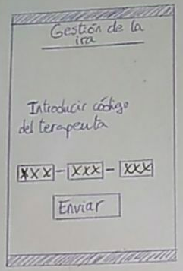
\includegraphics[width=0.8\linewidth, height=7cm]{Imagenes/anxA1-1.png}
        \caption[Mockup para iniciar sesión en la aplicación (versión I)]{Mockup para iniciar sesión en la aplicación (versión I)}
        \label{fig:c4:mockup1}
    \end{minipage}
    \hfill\vline\hfill
    \begin{minipage}{.45\textwidth}
        \centering
        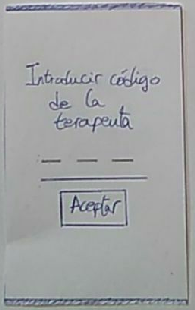
\includegraphics[width=0.8\linewidth, height=7cm]{Imagenes/anxA1-5.png}
        \caption[Mockup para iniciar sesión en la aplicación (versión II)]{Mockup para iniciar sesión en la aplicación (versión II)}
        \label{fig:c4:mockup2}
    \end{minipage}
\end{figure}

\paragraph{}
En la figura~\ref{fig:c4:mockup3}, aparece la pantalla con el nivel actual de ira del paciente. Si el paciente tiene un nivel de ira elevado (se encuentra inmerso en un episodio de ira) en esta pantalla también aparecen la pauta recomendada y la opción para introducir un comentario (por ejemplo, si decide no seguir la pauta recomendada).

\paragraph{}
La pantalla de la figura~\ref{fig:c4:mockup4} es una alternativa de las pantallas que aparecen en las figuras~\ref{fig:c4:mockup3},~\ref{fig:c4:mockup5} y~\ref{fig:c4:mockup6}, en el que la pantalla en la que aparece el nivel de ira y las pautas recomendadas se combina con la pantalla para sincronizar el dispositivo.

\begin{figure}[h]
    \centering
    \begin{minipage}{.4\textwidth}
        \centering
        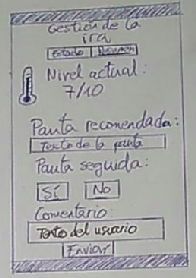
\includegraphics[width=0.8\linewidth, height=7cm]{Imagenes/anxA1-2.png}
        \caption[Mockup para ver el estado de ira y la pauta recomendada (versión II)]{Mockup para ver el estado de ira y la pauta recomendada (versión II)}
        \label{fig:c4:mockup3}
    \end{minipage}
    \hfill\vline\hfill
    \begin{minipage}{.4\textwidth}
        \centering
        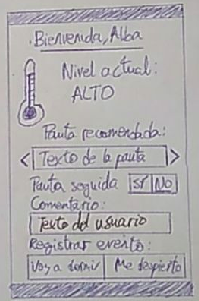
\includegraphics[width=0.8\linewidth, height=7cm]{Imagenes/anxA1-4.png}
        \caption[Mockup para ver el estado de ira y la pauta recomendada (versión I)]{Mockup para ver el estado de ira y la pauta recomendada (versión I)}
        \label{fig:c4:mockup4}
    \end{minipage}%
\end{figure}

\paragraph{}
En la figura~\ref{fig:c4:mockup5} aparece la pantalla para calibrar la pulsera en la que el paciente debe seleccionar si se va a dormir o a despertar. Una vez sincronizada la pulsera, esta pantalla ya no vuelve a aparecer. Esta pantalla es la única con la que podrá interactuar el usuario hasta que haya sincronizado el dispositivo, puesto que cada persona tiene unas constantes vitales distintas y sin esta información no es posible detectar los episodios de ira del paciente.

\paragraph{}
La pantalla de la figura~\ref{fig:c4:mockup6} es la segunda opción que se dio para la pantalla de la figura~\ref{fig:c4:mockup5}, cuya variación reside principalmente en darle al usuario la información de la hora a la que se acostó y se despertó para que así en caso de que haya sido introducido por error, esta información le ayude a dilucidarlo.

\begin{figure}[h]
    \centering
    \begin{minipage}{.4\textwidth}
        \centering
        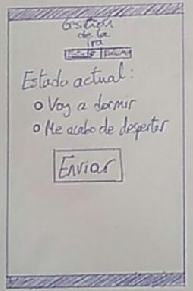
\includegraphics[width=0.8\linewidth, height=7cm]{Imagenes/anxA1-3.png}
        \caption[Mockup para calibrar el dispositivo (versión I)]{Mockup para calibrar el dispositivo (versión I)}
        \label{fig:c4:mockup5}
    \end{minipage}
    \hfill\vline\hfill
    \begin{minipage}{.4\textwidth}
        \centering
        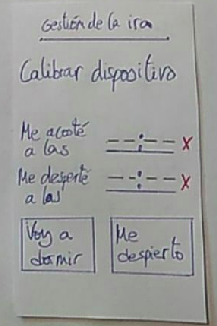
\includegraphics[width=0.8\linewidth, height=7cm]{Imagenes/anxA1-6.png}
        \caption[Mockup para calibrar el dispositivo (versión I)]{Mockup para calibrar el dispositivo (versión I)}
        \label{fig:c4:mockup6}
    \end{minipage}
\end{figure}

\paragraph{}
Una vez creados los prototipos en papel, se fijó una reunión con la psicóloga en la que se presentaron las distintas alternativas. Las principales conclusiones que se obtuvo de esta reunión fueron las siguientes:
\begin{itemize}
    \item La manera de emparejar la pulsera y el paciente que aparece en la figura~\ref{fig:c4:mockup2} es apropiada.
    \item Las dos alternativas para calibrar el dispositivo que se observan en las figuras~\ref{fig:mock5} y~\ref{fig:mock6} son apropiadas. No ve ninguna razón de peso para elegir una u otra, por lo que finalmente se optó por la alternativa de la figura~\ref{fig:c4:mockup6}, ya que le facilita más información al usuario y le permite rectificar la acción si pulsó accidentalmente alguno de los botones de la pantalla.
    \item El termómetro es una buena opción deberá aparecer en horizontal, estando el menor nivel de ira a la izquierda y el mayor en el otro extremo del termómetro, siguiendo la direccionalidad de la lectura en castellano.
    \item Para indicar el grado de ira, es mejor hacerlo con palabras (como en la figura~\ref{fig:c4:mockup2}) que de manera numérica (como en la figura~\ref{fig:c4:mockup1}). Los estados que discreticen el grado de ira que verá el paciente deberán ser reducidos para que el paciente pueda identificar su ordinalidad con facilidad. Así, la solución se limitará a cinco estados.
    \item Cuando varíe el grado de ira en el termómetro, no solo debe variar cuánto de lleno se encuentra éste, sino también su color. La terapeuta indicó que, tal y como comenta Valdez (\citeyear{valdez1994effects}), existe una relación estrecha entre emociones y colores, por lo que establecer por ejemplo que el rojo es el estado de calma y el verde es el estado de mayor percepción de la ira es un cambio significativo respecto a la asociación opuesta. En estudios experimentales se ha podido comprobar que los colores de mayor longitud de onda como son el rojo o el amarillo provocan mayor activación que otros de menor longitud de onda como es el verde. A su vez, Jacobs y Sues (\citeyear{jacobs1975effects}) han comprobado en un estudio con los colores rojo, amarillo, verde y azul que existe una mayor asociación del estrés con los colores rojo y amarillo respecto al verde y el azul. Así, a la hora de representar los colores asociados a cada nivel de ira, los colores asociados a estos niveles deberían ser (de menor a mayor nivel de ira): verde, verde-amarillo, amarillo, amarillo-rojo, rojo.
    \item Es importante que el paciente pueda cambiar de pauta si esta no le es útil.
    \item El comentario de las pautas debe ser opcional y se debe poder añadir usando la voz.
    \item Se deben incluir elementos sonoros que incrementen su volumen en función del nivel de ira del paciente para que este pueda ser consciente de que ha aumentado su nivel de ira.
    \item En la pantalla de la gestión de la ira se debe permitir al paciente seleccionar el tipo de situación que ha generado la ira.
\end{itemize}

\subsubsection{Diseño de la aplicación web del terapeuta}

\paragraph{}
El elemento de la figura~\ref{fig:c4:mockup7} sirve para mostrar cómo sería el inicio de sesión.

\paragraph{}
El elemento de la figura~\ref{fig:c4:mockup8} muestra una pantalla estándar para registrar a un paciente. El combo para seleccionar el grupo finalmente fue descartado.

\paragraph{}
El elemento de la figura~\ref{fig:c4:mockup9} muestra cómo se crearían grupos y se modificaría su composición de pacientes.

\paragraph{}
En las figuras~\ref{fig:c4:mockup10} y~\ref{fig:c4:mockup11} se muestran dos alternativas para mostrar las pautas: una única tabla para todos los niveles de activación en la que se cuenta con una columna del porcentaje de efectividad general entre los pacientes y una segunda con el texto de la pauta. La primera opción es más visual y cuenta con menos información: no se incluye la columna del porcentaje de éxito de cada pauta y las pautas están divididas en tablas según el nivel de activación asociado.

\begin{figure}[h]
    \centering
    \begin{minipage}{.4\textwidth}
        \centering
        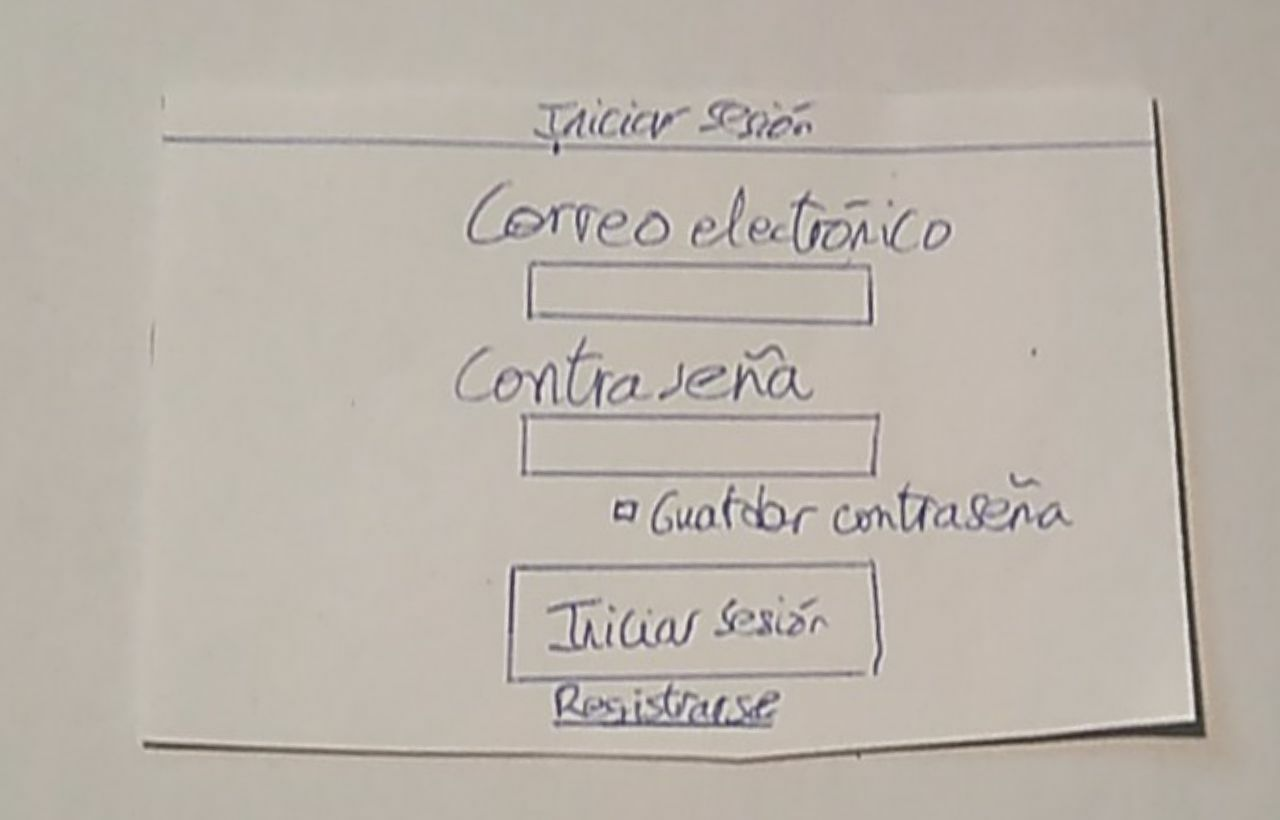
\includegraphics[width=0.8\linewidth, height=7cm]{Imagenes/anxA2.jpg}
        \caption[Mockup para iniciar sesión en la web]{Mockup para iniciar sesión en la web}
        \label{fig:c4:mockup7}
    \end{minipage}
    \hfill\vline\hfill
    \begin{minipage}{.4\textwidth}
        \centering
        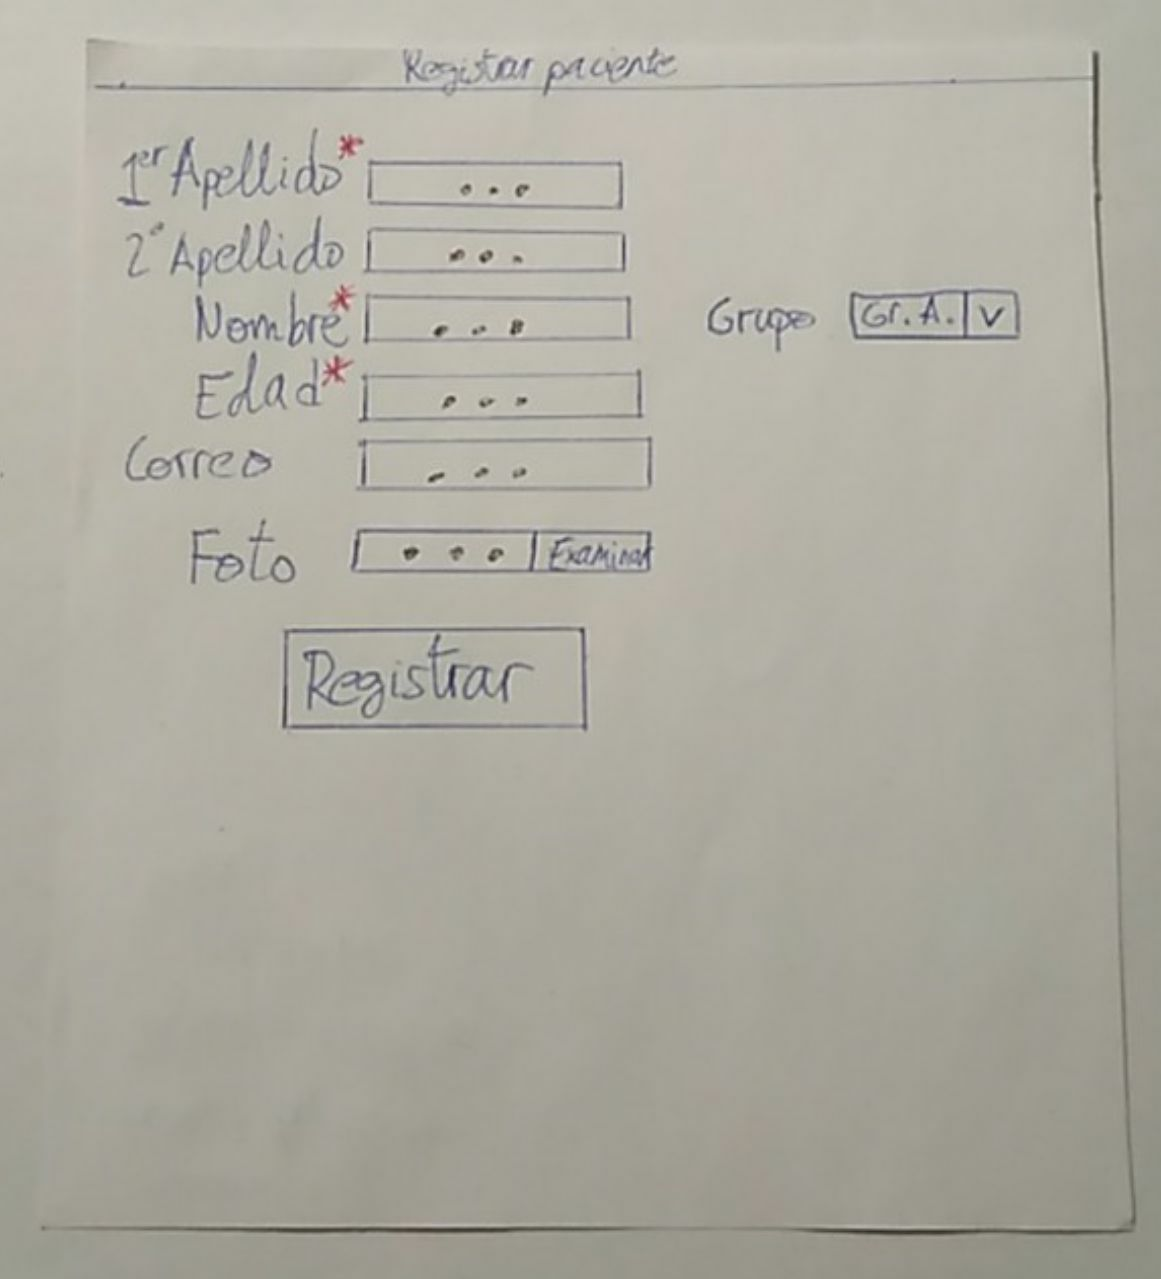
\includegraphics[width=0.8\linewidth, height=7cm]{Imagenes/anxA3.jpg}
        \caption[Mockup para registrar al paciente en la web]{Mockup para registrar al paciente en la web}
        \label{fig:c4:mockup8}
    \end{minipage}
\end{figure}

\paragraph{}
En la figura~\ref{fig:c4:mockup12} aparece una pantalla genérica para modificar el paciente en la que a su vez aparece la información asociada a las pautas que le han ido apareciendo en la aplicación móvil.

\paragraph{}
En las figuras~\ref{fig:c4:mockup13},~\ref{fig:c4:mockup14} y~\ref{fig:c4:mockup15} aparecen las tres opciones que se presentaban a la terapeuta para cada paciente en el que se podía ver el resumen de episodios de cada paciente. Dos de ellos consisten en tablas en las que en una aparece las pautas que se recomendaban y en el otro si la pauta suministrada funcionó o no. La opción alternativa era mostrar una gráfica con los distintos episodios acaecidos en un periodo de tiempo.


\begin{figure}[h]
    \centering
    \begin{minipage}{.45\textwidth}
        \centering
        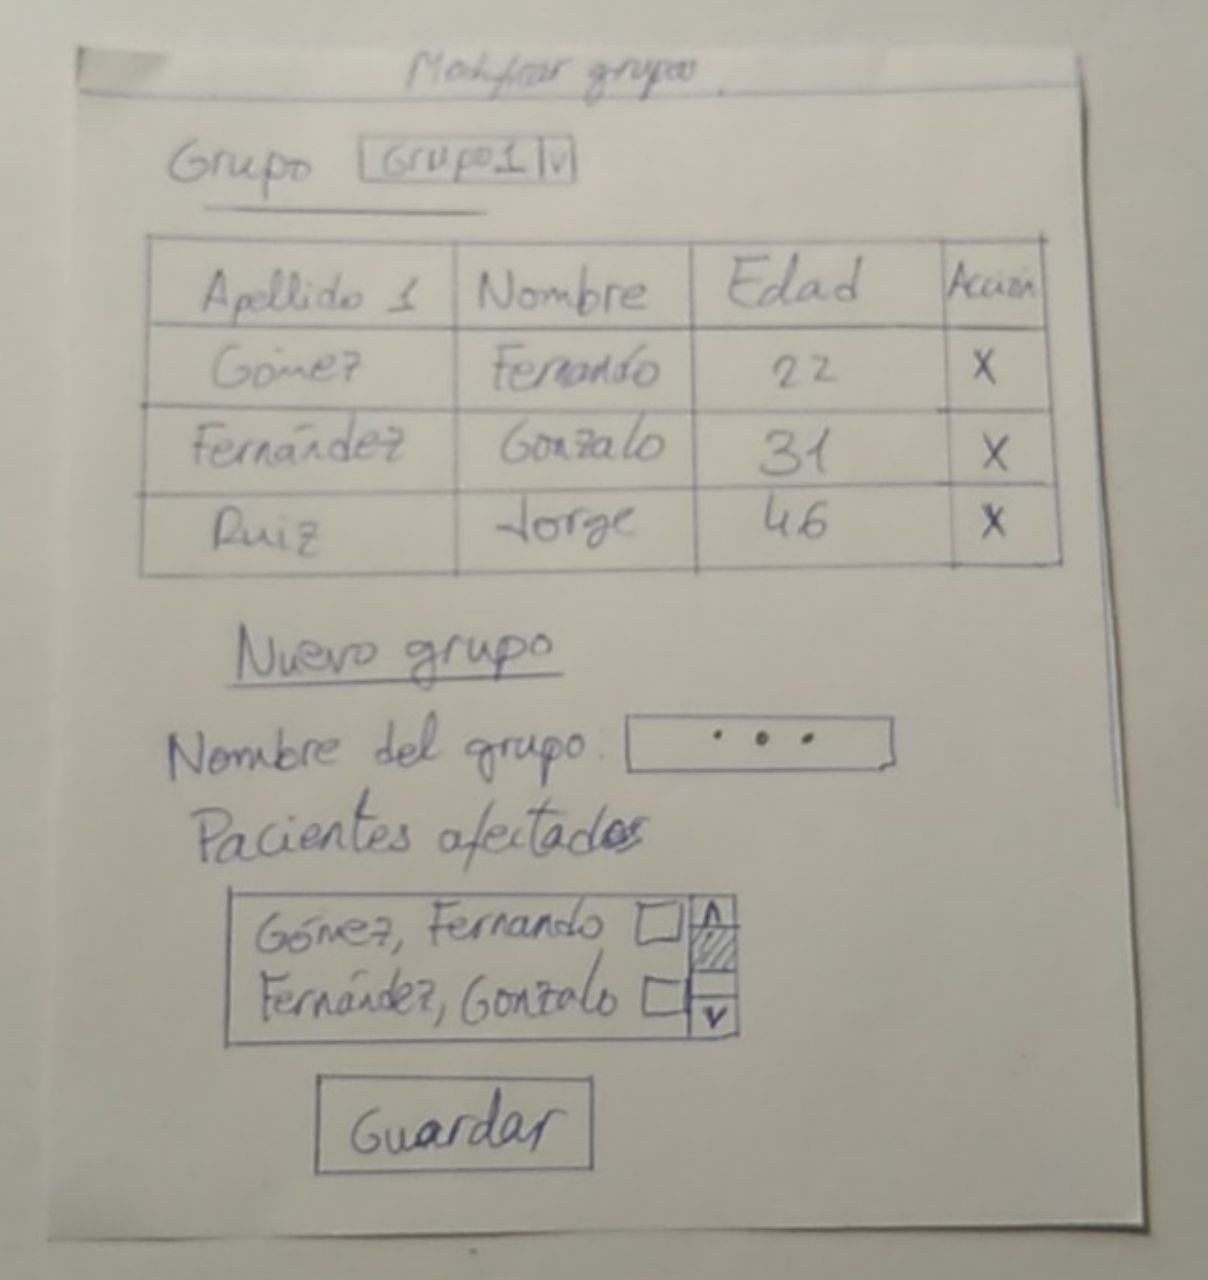
\includegraphics[width=0.8\linewidth, height=7cm]{Imagenes/anxA4.jpg}
        \caption[Mockup para la gestión de grupos de pacientes]{Mockup para la gestión de grupos de pacientes}
        \label{fig:c4:mockup9}
    \end{minipage}
    \hfill\vline\hfill
    \begin{minipage}{.45\textwidth}
        \centering
        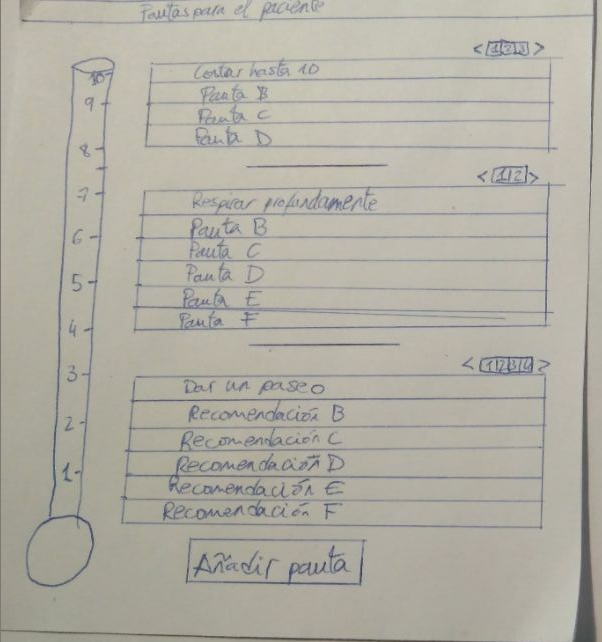
\includegraphics[width=0.8\linewidth, height=7cm]{Imagenes/anxA5-1.png}
        \caption[Mockup para la gestión de pautas (versión I)]{Mockup para la gestión de pautas (versión I)}
        \label{fig:c4:mockup10}
    \end{minipage}
\end{figure}

\paragraph{}
En la figura~\ref{fig:c4:mockup16} aparece un elemento genérico para incluir en la cabecera de la pantalla del usuario con información básica sobre este. Al pulsar sobre el botón modificar, se redireccionaría la a pantalla de la figura~\ref{fig:c4:mockup12}.

\begin{figure}[h]
    \centering
    \begin{minipage}{.45\textwidth}
        \centering
        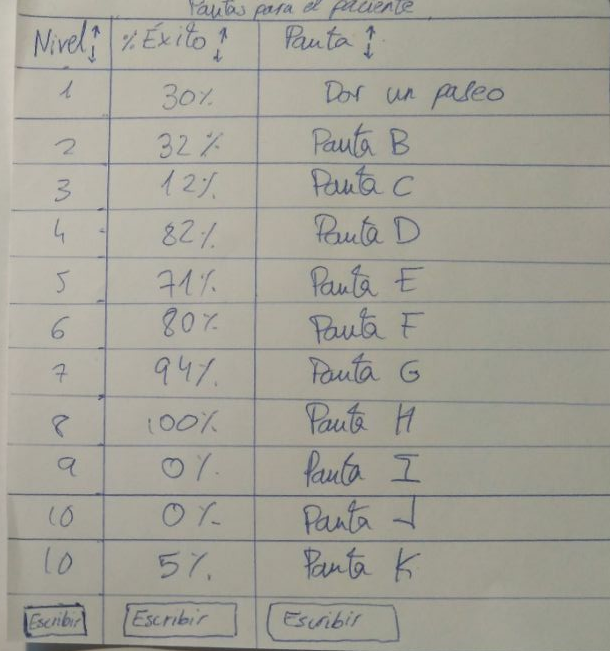
\includegraphics[width=0.8\linewidth, height=7cm]{Imagenes/anxA5-2.png}
        \caption[Mockup para la gestión de pautas (versión II)]{Mockup para la gestión de pautas (versión II)}
        \label{fig:c4:mockup11}
    \end{minipage}
    \hfill\vline\hfill
    \begin{minipage}{.45\textwidth}
        \centering
        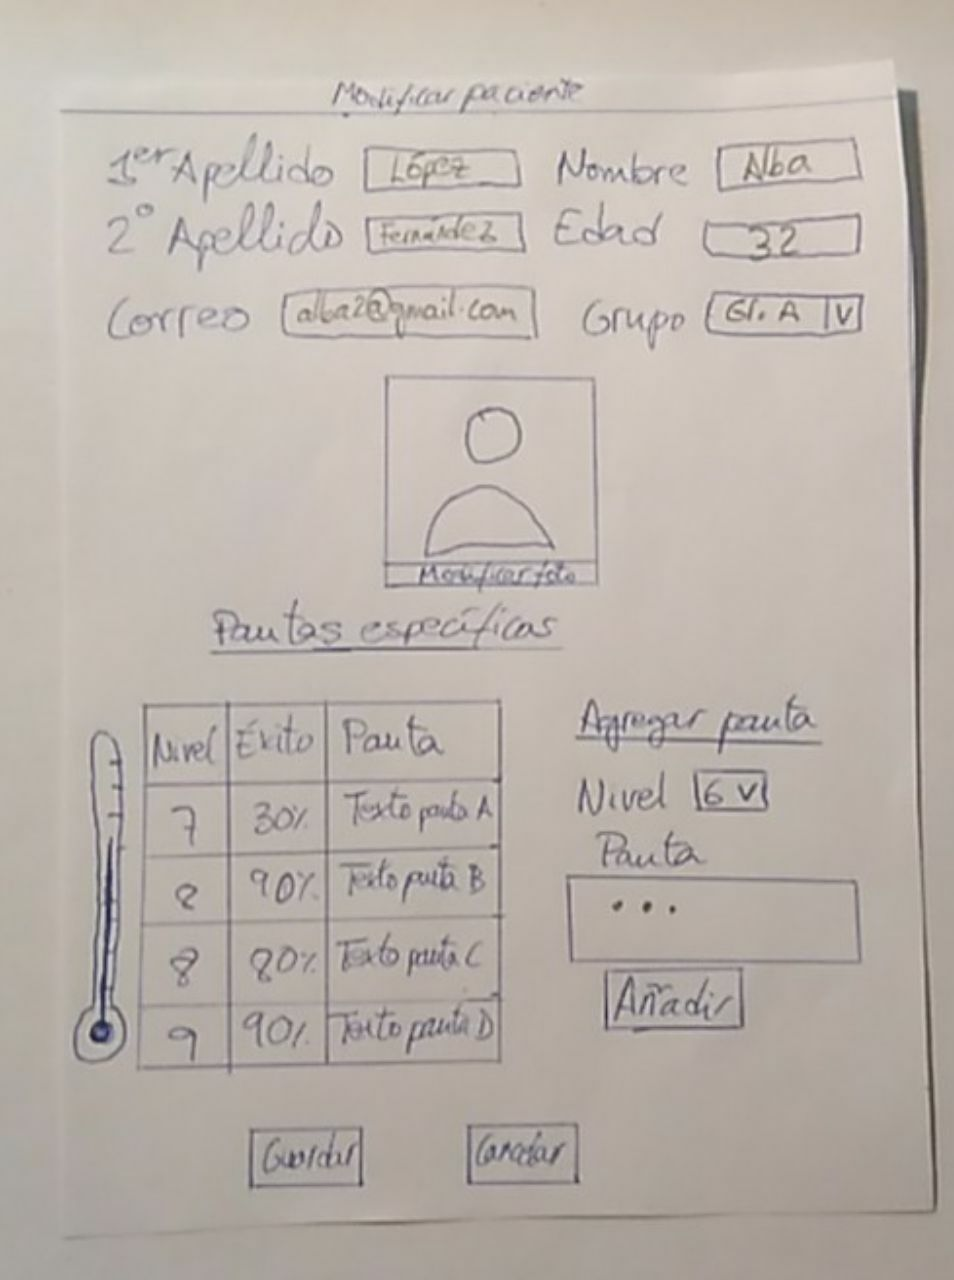
\includegraphics[width=0.8\linewidth, height=7cm]{Imagenes/anxA6.jpg}
        \caption[Mockup para la gestión de un paciente]{Mockup para la gestión de un paciente}
        \label{fig:c4:mockup12}
    \end{minipage}
\end{figure}

\paragraph{}
En la figura~\ref{fig:c4:mockup17} aparecen los dos elementos que se utilizarían tanto en la pantalla principal con el resumen de alertas de todos los pacientes como en la pantalla particular de cada paciente. El botón \textit{ver detalles} llevaría a una tabla o gráfica con el resumen de episodios citados.

\paragraph{}
En la figura~\ref{fig:c4:mockup18} aparece el resumen de los episodios de todos los pacientes en el periodo especificado en el segundo elemento de la figura anterior. Así, el elemento más a la izquierda sería un filtro de pacientes similar al que se encuentra en páginas web de compra de artículos en la que se podría filtrar a los mismos en función de la información que se tiene de ellos, así como se podría hacer usando el buscador horizontal que se encuentra en la parte superior de la imagen. Al pulsar sobre cualquiera de estas filas, se abriría la página con el resumen de episodios del paciente seleccionado. La diferencia entre ambas tablas reside principalmente en la utilización del espacio y en que la información provista sea menos o más visual: la opción más a la izquierda, a diferencia de lo que ocurre con la opción de la derecha, no incluiría fotografía y estaría pensada para ocupar menos espacio vertical por registro, lo que permitiría poder representar más registros en el mismo espacio respecto a la segunda opción.

\begin{figure}
    \centering
    \begin{minipage}{.45\textwidth}
        \centering
        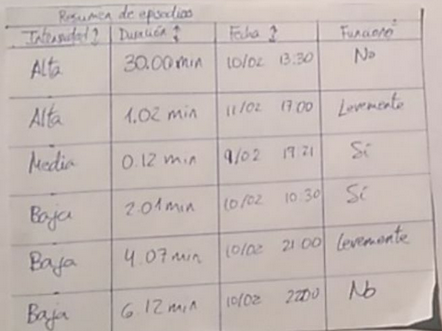
\includegraphics[width=0.8\linewidth, height=7cm]{Imagenes/anxA7-1.png}
        \caption[Mockup para mostrar los episodios de un paciente (versión I)]{Mockup para mostrar los episodios de un paciente (versión I)}
        \label{fig:c4:mockup13}
    \end{minipage}
    \hfill\vline\hfill
    \begin{minipage}{.45\textwidth}
        \centering
        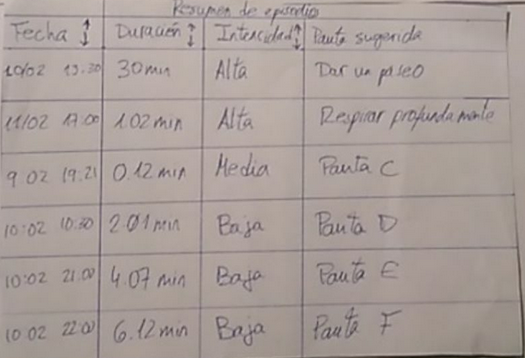
\includegraphics[width=0.8\linewidth, height=7cm]{Imagenes/anxA7-2.png}
        \caption[Mockup para mostrar los episodios de un paciente (versión II)]{Mockup para mostrar los episodios de un paciente (versión II)}
        \label{fig:c4:mockup14}
    \end{minipage}
\end{figure}

\paragraph{}
En la figura~\ref{fig:c4:mockup17} aparece el resumen de los episodios para todos los pacientes. Esto se incluiría en la página principal. La información es la misma, lo único que varía es su representación.

\begin{figure}
    \centering
    \begin{minipage}{.45\textwidth}
        \centering
        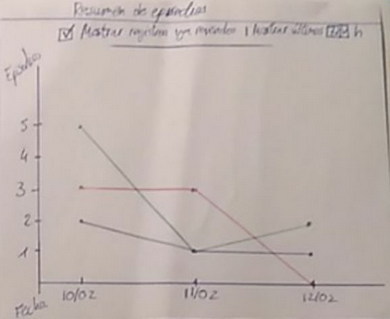
\includegraphics[width=0.8\linewidth, height=7cm]{Imagenes/anxA7-3.png}
        \caption[Mockup para mostrar los episodios de un paciente (versión III)]{Mockup para mostrar los episodios de un paciente (versión III)}
        \label{fig:c4:mockup15}
    \end{minipage}
\end{figure}


\begin{figure}[!htbp]
    \centering
    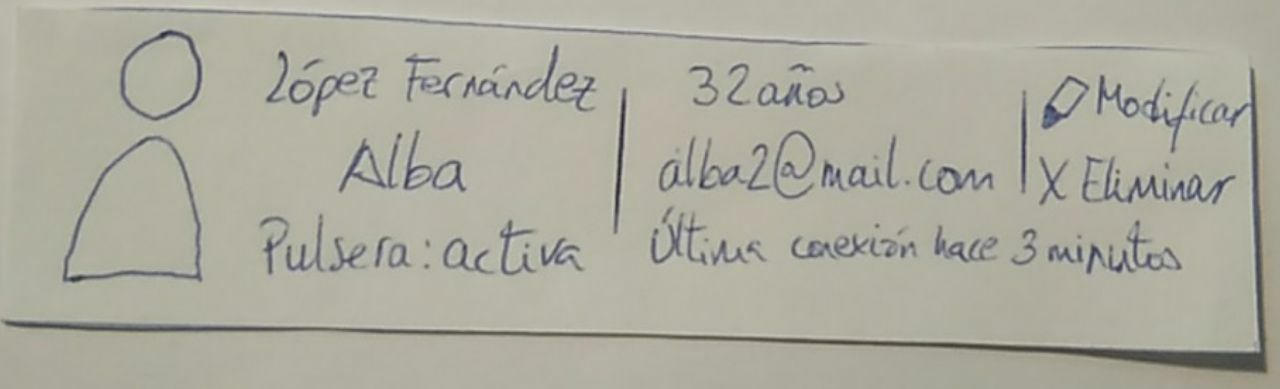
\includegraphics[scale=0.3]{Imagenes/anxA8.jpg}
    \caption[Mockup para mostrar la información básica del paciente]{Mockup para mostrar la información básica del paciente}
    \label{fig:c4:mockup16}
\end{figure}

\begin{figure}[!htbp]
    \centering
    %width=3cm, height=3cm
\begin{frame}{Frame Title}
    
\end{frame}[]    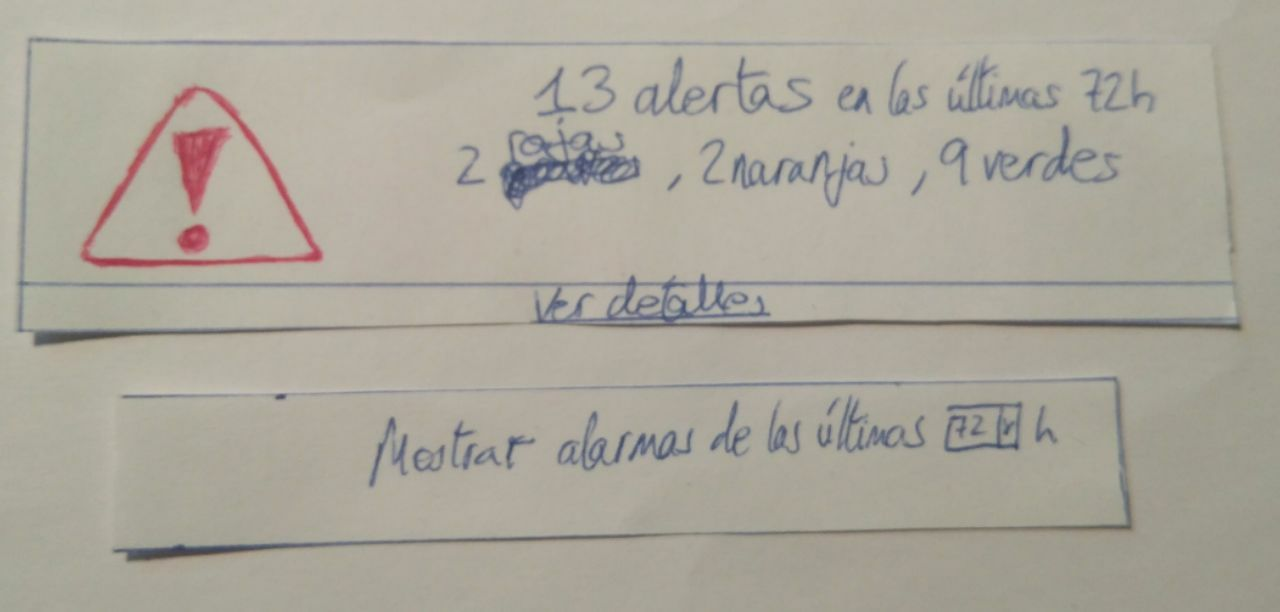
\includegraphics[scale=0.3]{Imagenes/anxA9.jpg}
    \caption[Mockup mostrar alertas de episodios de ira]{Mockup mostrar alertas de episodios de ira}
    \label{fig:c4:mockup17}
\end{figure}

\begin{figure}[!htbp]
    \centering
    %width=3cm, height=3cm
    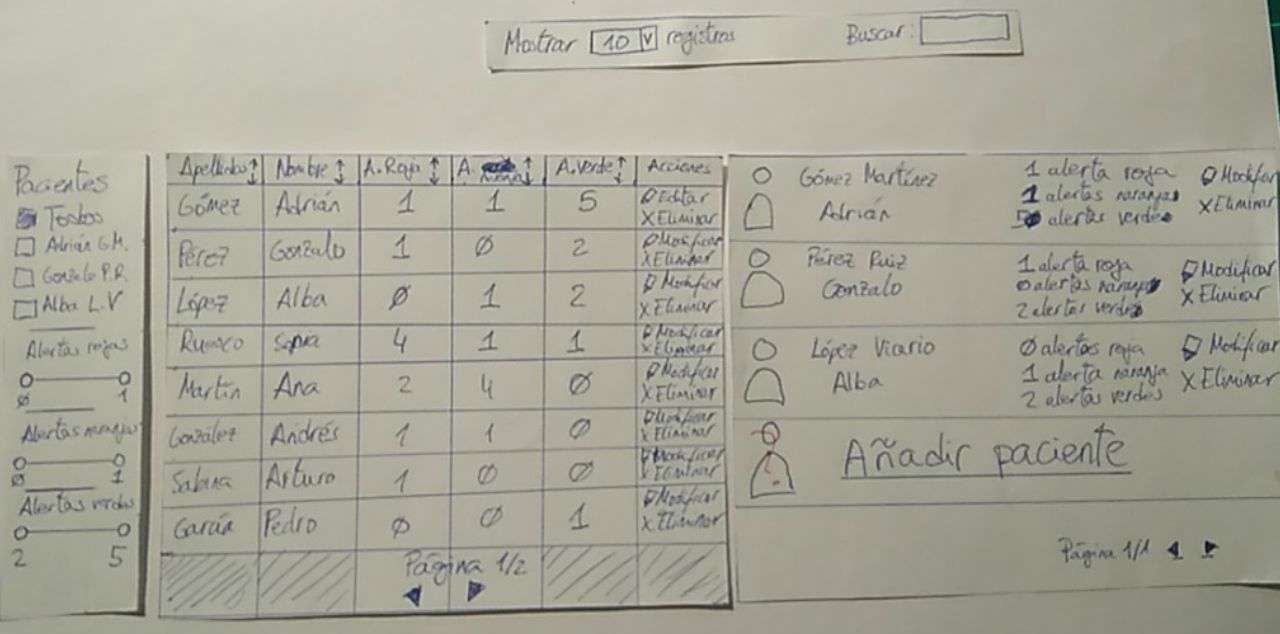
\includegraphics[scale=0.3]{Imagenes/anxA10.jpg}
    \caption[Mockup para mostrar los filtros y las dos opciones para mostrar la tabla de pacientes]{Mockup para mostrar los filtros y las dos opciones para mostrar la tabla de pacientes}
    \label{fig:c4:mockup18}
\end{figure}

\begin{figure}
    \centering
    \begin{minipage}{.45\textwidth}
        \centering
        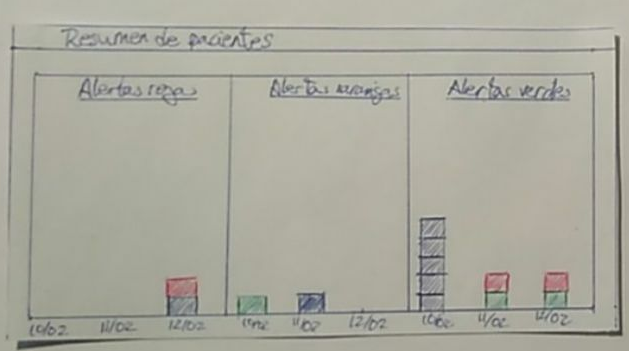
\includegraphics[width=0.8\linewidth, height=7cm]{Imagenes/anxA11-1.png}
        \caption[Mockup para mostrar el resumen de alertas de los pacientes (versión I)]{Mockup para mostrar el resumen de alertas de los pacientes (versión I)}
        \label{fig:c4:mockup19}
    \end{minipage}
    \hfill\vline\hfill
    \begin{minipage}{.45\textwidth}
        \centering
        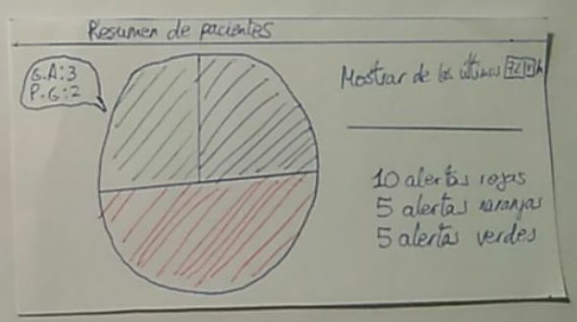
\includegraphics[width=0.8\linewidth, height=7cm]{Imagenes/anxA11-2.png}
        \caption[Mockup para mostrar el resumen de alertas de los pacientes (versión II)]{Mockup para mostrar el resumen de alertas de los pacientes (versión II)}
        \label{fig:c4:mockup20}
    \end{minipage}
\end{figure}

\paragraph{}
Una vez creados los prototipos en papel de la aplicación web, nos reunimos con la terapeuta para mostrarselos y buscar el diseño que mejor se ajustase a las necesidades de los usuarios finales. Las principales conclusiones que se obtuvo de esta reunión fueron las siguientes:

\begin{itemize}
    \item El método de autentificación del terapeuta para iniciar sesión con la tupla correo electrónico y contraseña es apropiado.
    \item A la hora de registrar un paciente,es apropiado poder incluir las fotos de pacientes para mejorar la visualización. El correo electrónico no es necesario y el grupo al que pertenece cada paciente es prescindible. Para futuras versiones podría ser interesante agrupar a los pacientes y obtener resultados globales de estos grupos pero para esta versión se acaba decidiendo que es mejor centrarse en una solución más sencilla. Por ello, la figura~\ref{fig:c4:mockup3} debe suprimir la selección del grupo y la pantalla de la figura~\ref{fig:c4:mockup4} no tiene que aparecer.
    \item Entre el primer y segundo elemento de la figura~\ref{fig:c4:mockup18} para representar las pautas de cada paciente, se considera que la solución tiene que ser algo intermedio: conservar la estructura del primer elemento de dividir las pautas en diversas tablas según su grado de intensidad (con un termómetro en paralelo para poder correlacionar fácilmente la intensidad de cada pauta) pero añadiendo columnas adicionales a las pautas como por ejemplo el porcentaje de éxito, tal y como se ve en el segundo elemento.
    \item Se considera apropiado que en el resumen de los episodios de ira figure el tiempo que se mantuvo el paciente en cada uno de los estados, tal y como aparece en el primer elemento de la figura~\ref{fig:c4:mockup14}.
    \item La información de la pauta recomendada para cada episodio, tal y como aparece en el tercer elemento de la figura~\ref{fig:c4:mockup14} se considera apropiada, pero es incompleto, ya que para un mismo estado al paciente se le puede haber recomendado más de una pauta. El paciente puede haber descartado pautas previas, y esta información es importante que quede registrada.
    \item La figura~\ref{fig:c4:mockup15} muestra la representación los episodios en formato histograma, lo que es correcto. El gráfico de tarta que aparece en la gráfica ~\ref{fig:c4:mockup20} no aporta información útil, porque cómo se ha desarrollado el episodio es relevante, como por ejemplo el tiempo que ha pasado en cada estado. El segundo elemento de la figura~\ref{fig:c4:mockup7} hace una aproximación a esto pero es incompleto, puesto que es necesario que sea una gráfica interactiva que permita poder ampliarla para por ejemplo poder seleccionar solo un episodio e ir viéndolos uno a uno. Para este fin, la terapeuta propone basarse en el ejemplo de las gráficas de los desfibriladores.
    \item Las figuras~\ref{fig:c4:mockup17} y ~\ref{fig:c4:mockup18} son elementos adicionales que sirven para decorar las pantallas que se iban generando. La figura~\ref{fig:c4:mockup17} se considera apropiada mientras que el primer elemento de la figura~\ref{mockup18} se considera que no aporta información útil para la terapeuta.
    \item En la figura~\ref{fig:c4:mockup19} aparecen dos modelos de tablas y una serie de filtros para poder buscar los pacientes en dichas tablas. Los filtros se consideran apropiados, y ambos formatos de tablas también a excepción de las columnas que indican el número de alertas de cada una de las intensidades de la ira de cada paciente, ya que esta información sin estar agrupada en episodios y desglosada en fechas, no aporta información relevante al terapeuta.
\end{itemize}

\subsection{Segunda iteracción}

\paragraph{}
Para esta segunda iteracción, se usaron prototipos de alta fidelidad con Android y HTML para que estos fueran lo más similares posibles al resultado final de la aplicación. Esto se debe a que, tras la primera iteracción, se pudieron extraer los suficientes requisitos como para poder avanzar en detalles más concretos de la aplicación final.

\subsubsection{Diseño de la aplicación móvil de los pacientes}

\paragraph{}
Las pantallas de esta segunda fase para el móvil son las siguientes:

\begin{itemize}
    \item En la figura~\ref{fig:c4:mockup21} aparece la pantalla para introducir el código para sincronizar la pulsera y el móvil con el paciente. Es la equivalente de la fase anterior que aparece en la figura~\ref{fig:c4:mockup1}.
    \item En la figura~\ref{fig:c4:mockup22} podemos ver la pantalla para sincronizar el dispositivo durante su primer uso.
\end{itemize}

\begin{figure}[h]
    \centering
    \begin{minipage}{.45\textwidth}
        \centering
        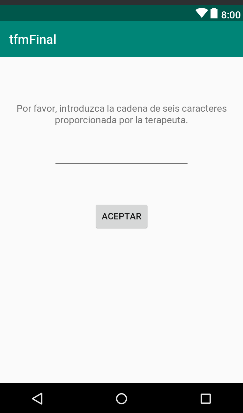
\includegraphics[width=0.8\linewidth, height=7cm]{Imagenes/anxA12.png}
        \caption[Mockup para sincronizar el dispositivo]{Mockup para sincronizar el dispositivo}
        \label{fig:c4:mockup21}
    \end{minipage}
    \hfill\vline\hfill
    \begin{minipage}{.45\textwidth}
        \centering
        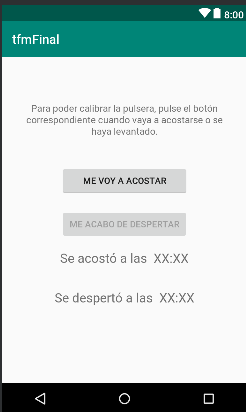
\includegraphics[width=0.8\linewidth, height=7cm]{Imagenes/anxA13.png}
        \caption[Mockup para calibrar el dispositivo]{Mockup para calibrar el dispositivo}
        \label{fig:c4:mockup22}
    \end{minipage}
\end{figure}

\begin{itemize}
    \item En la figura~\ref{fig:c4:mockup21} encontramos la que será la pantalla principal, donde aparece la pauta recomendada, el nivel de la ira representado mediante un termómetro horizontal, la posibilidad de cambiar de pauta y de enviar comentarios sobre la pauta en cuestión.
\end{itemize}

\begin{figure}[h]
    \centering
    \begin{minipage}{.45\textwidth}
        \centering
        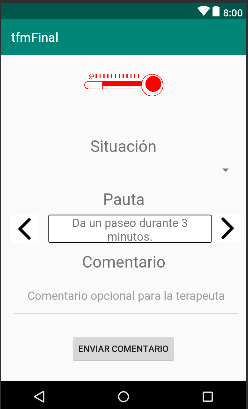
\includegraphics[width=0.8\linewidth, height=7cm]{Imagenes/anxA14.png}
        \caption[Mockup de la pantalla principal]{Mockup de la pantalla principal}
        \label{fig:c4:mockup23}
    \end{minipage}
    \hfill\vline\hfill
    \begin{minipage}{.45\textwidth}
        \centering
        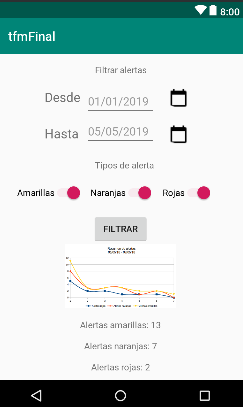
\includegraphics[width=0.8\linewidth, height=7cm]{Imagenes/anxA15.png}
        \caption[Mockup del histórico de episodios de un paciente]{Mockup del histórico de episodios de un paciente}
        \label{fig:c4:mockup24}
    \end{minipage}
\end{figure}

\begin{itemize}

    \item En la figura~\ref{fig:c4:mockup24} se encuentra una pantalla de resumen de la evolución seguida por el paciente. Esto es una innovación respecto a la anterior versión puesto que la terapeuta comentó que esta información puede servir para motivar al paciente al poder verificar en un histograma cómo se han reducido sus episodios de ira.

\begin{figure}[h!]
    \centering
    \begin{minipage}{.45\textwidth}
        \centering
        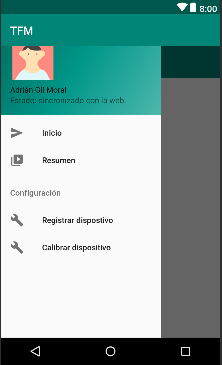
\includegraphics[width=0.8\linewidth, height=7cm]{Imagenes/anxA16.png}
        \caption[Mockup del menú de la aplicación]{Mockup del menú de la aplicación}
        \label{fig:c4:mockup25}
    \end{minipage}
\end{figure}

    \item En la figura~\ref{fig:c4:mockup25} se puede ver la manera que se utilizaría para cambiar entre las pantallas. En lugar de tener un menú horizontal que quite espacio para el resto de pantallas, este menú se desplegará como se hace en aplicaciones como Telegram o Whatsapp mediante el pulsado en un bocadillo a la izquierda de la barra horizontal superior o mediante el desplazamiento de la pantalla de izquierda a derecha.
\end{itemize}

\paragraph{}
Al revisar este diseño con la terapeuta, se obtuvieron las siguientes conclusiones:

\begin{itemize}
    \item Las pantallas que se muestran se ajustan bastante a lo esperado por parte de la terapeuta, pero en ellas aparece el concepto de alertas que debe desaparecer. Un episodio es un conjunto cronológicamente ordenado de alertas que empieza en el estado de reposo y acaba en el estado de reposo. Esa debe ser la unidad mínima con la que el terapeuta debe trabajar.
    \item El termómetro de la imágen debe ir al revés: el elemento de mayor grosor tiene que ir a la izquierda, que representará el menor nivel de ira.
    \item Se debe incluir un widget en la aplicación en el que aparezca un pequeño termómetro con el nivel de ira del paciente en ese momento para que el paciente pueda ver su estado actual de la ira sin necesidad de abrir la aplicación.
    \item Se deben incluir mensajes de alertas motivacionales tipo \textit{toast} como refuerzo positivo para el paciente cuando se detecte una disminución continuada de sus episodios de ira.
    \item A la hora de interpretar la actividad fisiológica del paciente, es necesario discernir entre actividades que puedan generar mayor activación que no impliquen episodios de ira (como al realizar ejercicio físico o al mantener relaciones sexuales) de aquellas que sean fruto de un estado de ira.
    \item En esta interacción se ha echado en falta poder ver cómo quedaría la pantalla principal de la figura~\ref{fig:c4:mockup23} cuando el paciente no está experimentando un episodio de ira.
    \item En la pantalla principal que aparece en la figura~\ref{fig:c4:mockup23} es necesario que no solo aparezca la pauta que se recomienda seguir para reducir el nivel de ira, sino que también es necesario que el paciente pueda seleccionar entre una lista de opciones la causa principal que ha generado la ira.
    \item En la pantalla que aparece en la figura~\ref{fig:c4:mockup23} hay que añadir una función para que, después de un tiempo, pregunte al usuario si ha seguido la pauta que se ha recomendado. Si responde afirmativamente y el paciente no se encuentra en estado de reposo, se le mostrarán más pautas acordes a su nivel actual de ira. Si responde negativamente, se seguirá el mismo procedimiento pero preguntando al paciente por qué no ha seguido la pauta antes de mostrar la siguiente pauta. Esta información será de utilidad en la consulta para poder afinar el conjunto de pautas asociado a cada paciente.
\end{itemize}

\subsubsection{Diseño de la aplicación web del terapeuta}
\paragraph{}
En este caso, se diseñaron exclusivamente las pantallas que pudieran ser fruto de mayor controversia, eliminando pantallas estándar como las de inicio de sesión o modificación de pacientes, puesto que la interfaz de estas funcionalidades ya quedó cerrada en la iteracción anterior.

\paragraph{}
En la figura ~\ref{fig:c4:mockup26} podemos ver la pantalla principal, que sería la implementación de los elementos de la figura ~\ref{fig:c4:mockup11}.

\begin{figure}[h]
    \centering
    %width=3cm, height=3cm
    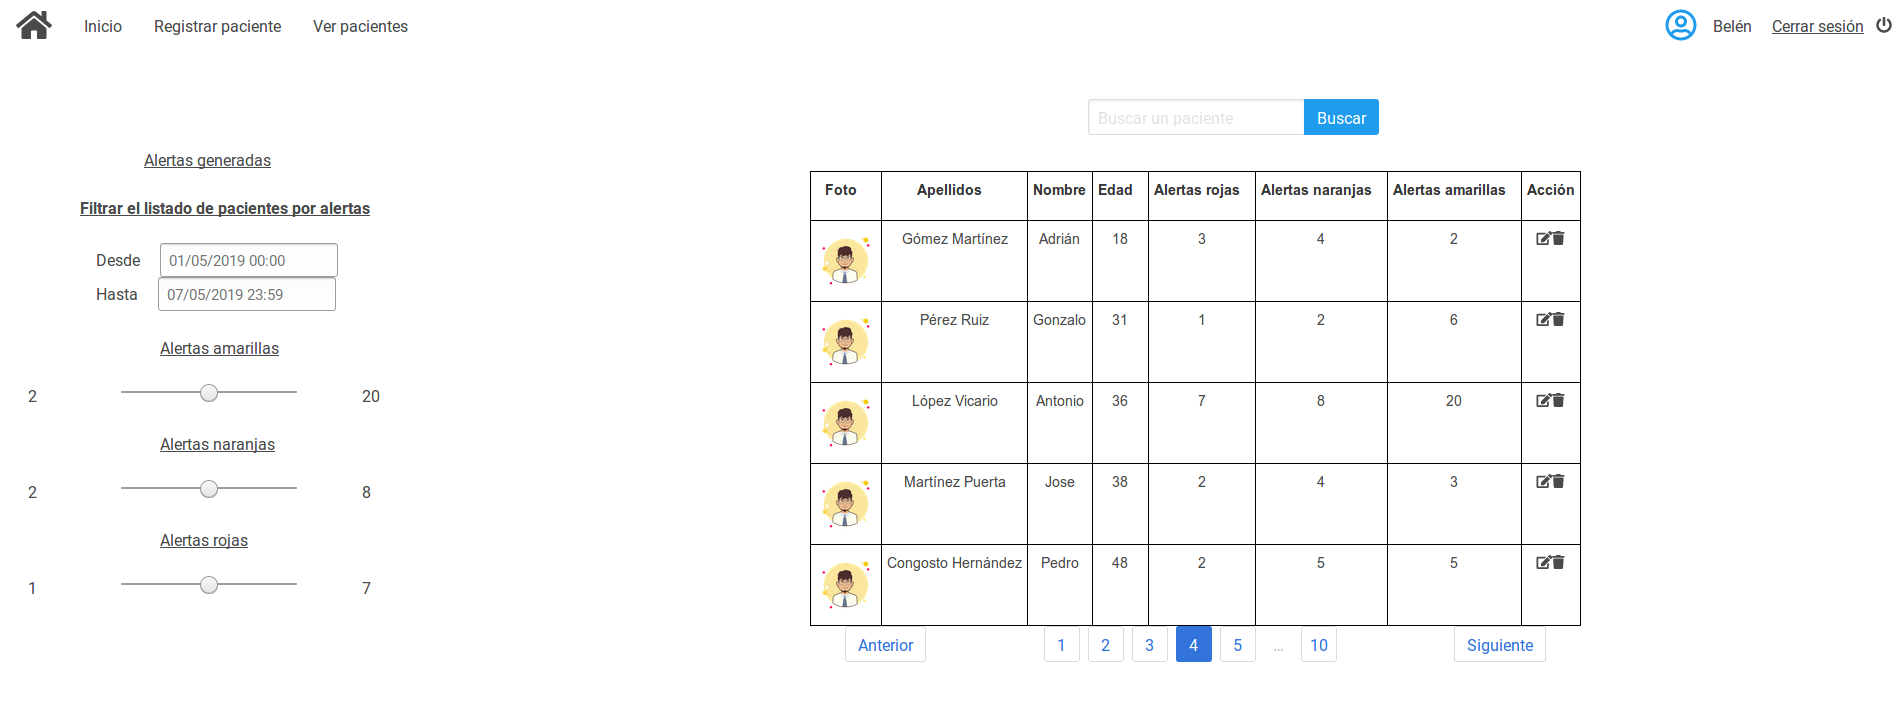
\includegraphics[height=7.5cm, width=\textwidth]{Imagenes/anxA17.png}
    \caption[Mockup de la pantalla principal de la web]{Mockup de la pantalla principal de la web}
    \label{fig:c4:mockup26}
\end{figure}

\paragraph{}
En las figuras~\ref{fig:c4:mockup27} y~\ref{fig:c4:mockup28} se puede ver la pantalla en la que aparecería el resumen de cada paciente mediante una gráfica y una tabla de formato acordeón a continuación con información detallada de cada uno de los estados del episodio por los que ha pasado el paciente.

\begin{figure}[!htbp]
    \centering
    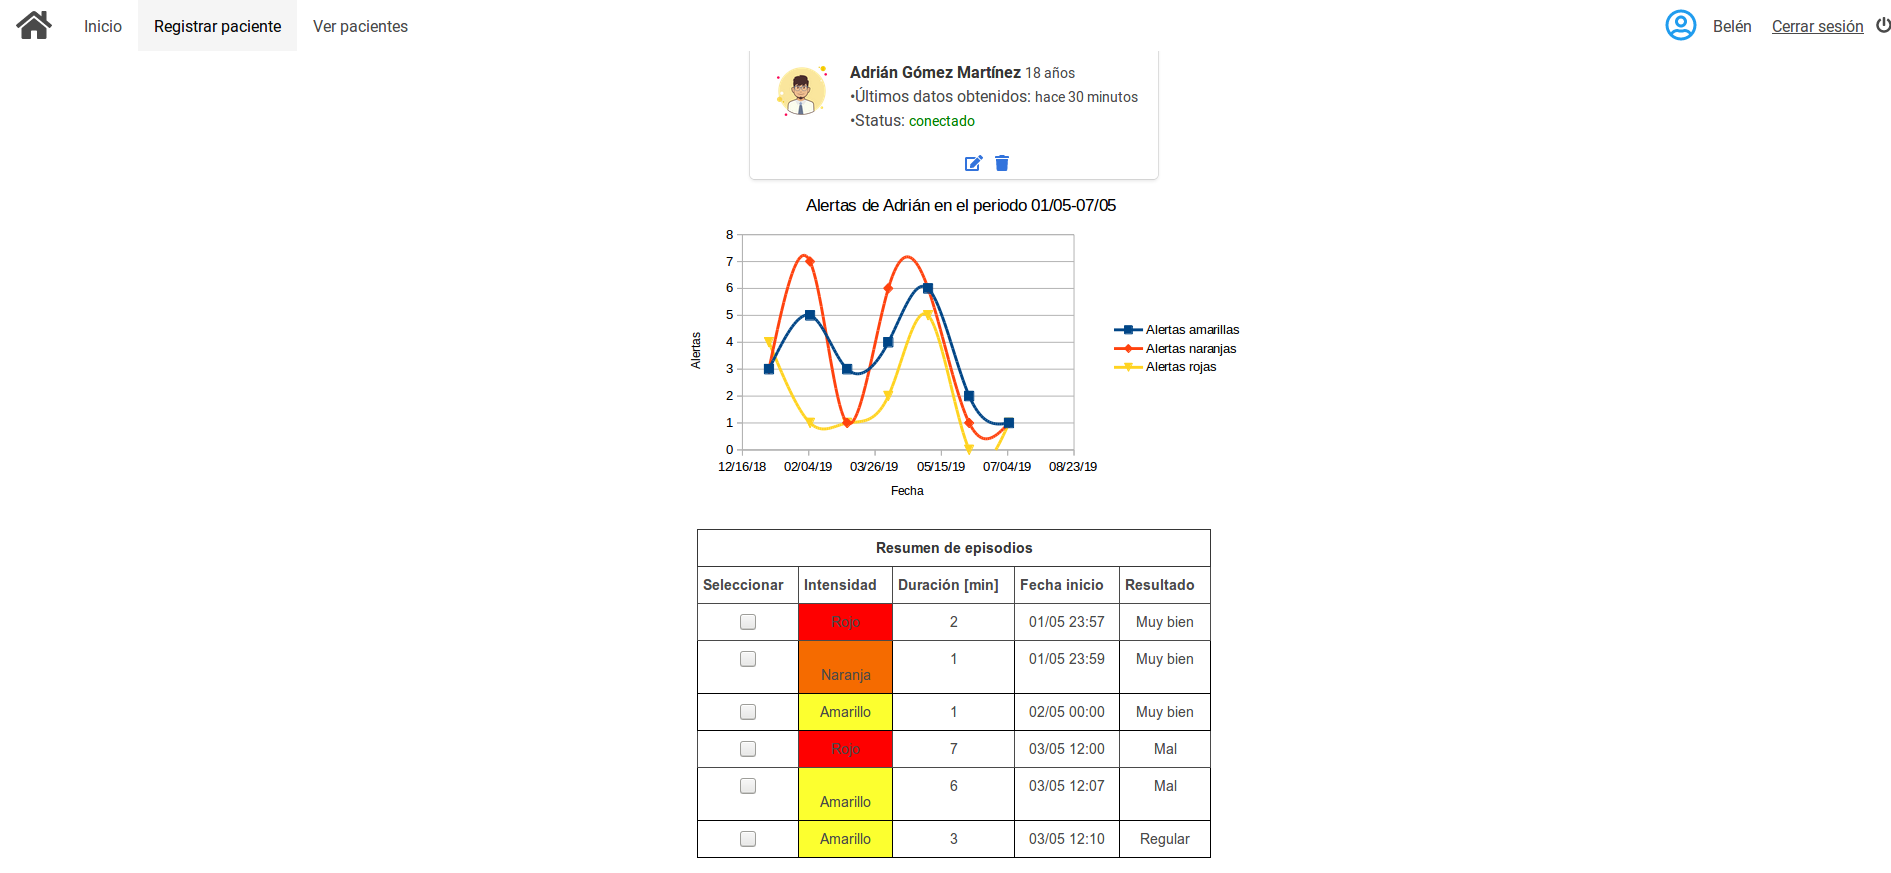
\includegraphics[height=7.5cm, width=\textwidth]{Imagenes/anxA18.png}
    \caption[Mockup de la pantalla para ver los episodios (I/II)]{Mockup de la pantalla para ver los episodios (I/II)}
    \label{fig:c4:mockup27}
\end{figure}

\begin{figure}[!htbp]
    \centering
    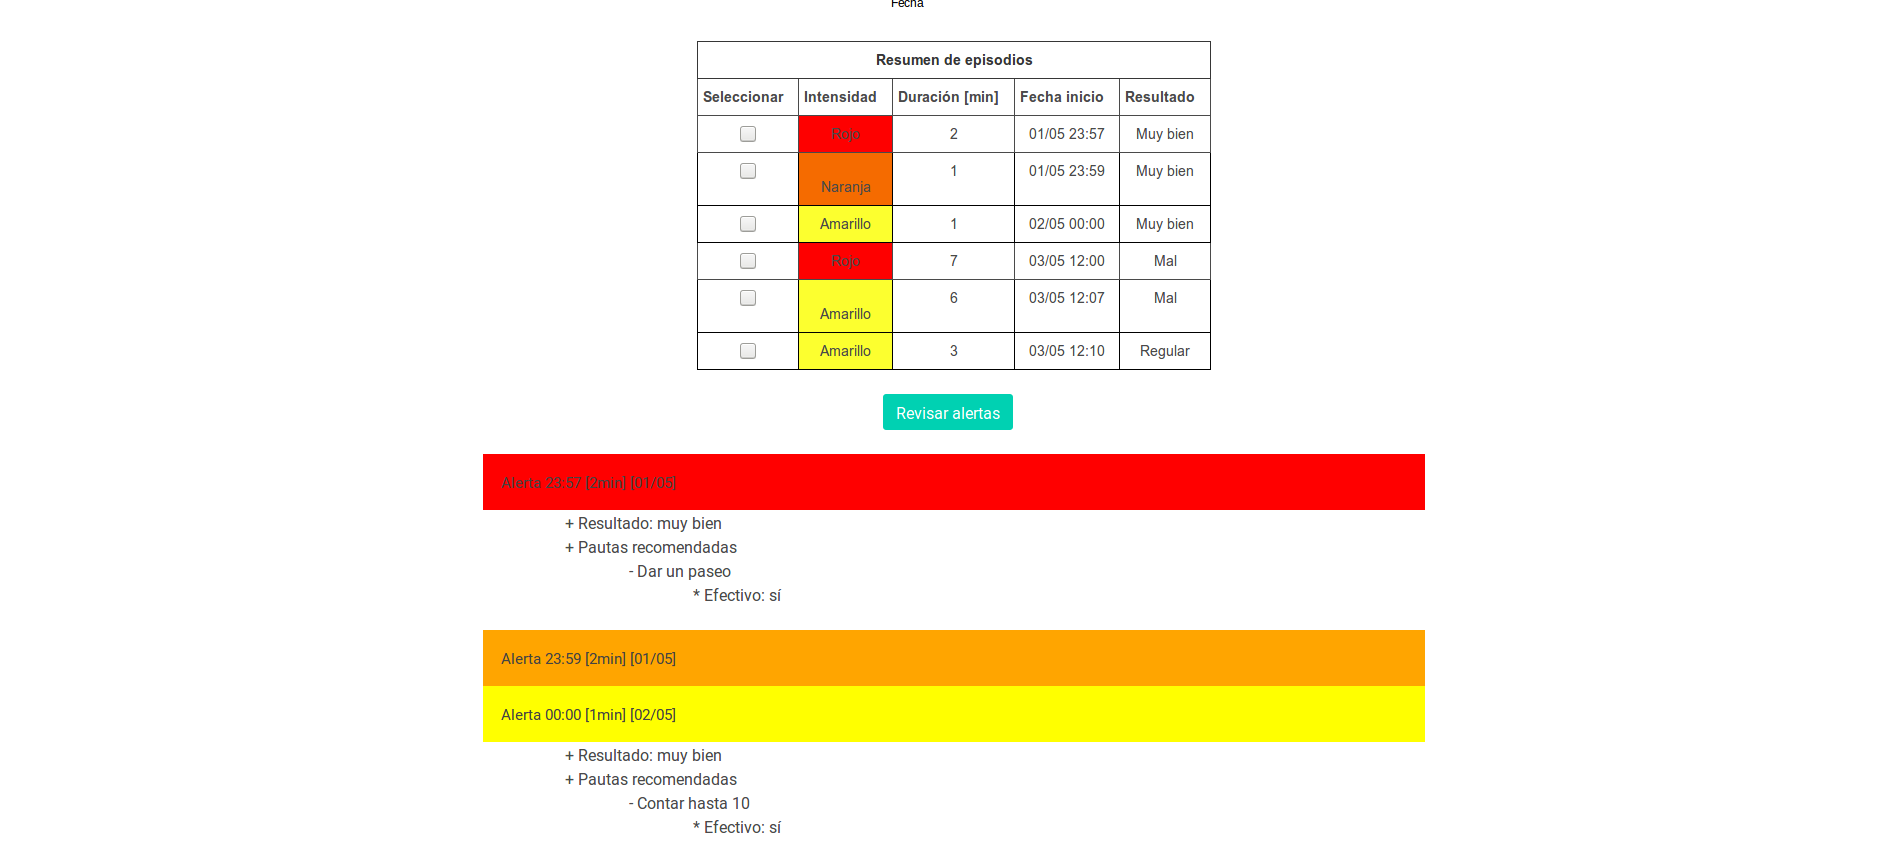
\includegraphics[height=7.5cm, width=\textwidth]{Imagenes/anxA19.png}
    \caption[Mockup de la pantalla para ver los episodios (II/II)]{Mockup de la pantalla para ver los episodios (II/II)}
    \label{fig:c4:mockup28}
\end{figure}

\paragraph{}
En la figura ~\ref{fig:c4:mockup25} se puede ver la implementación de la pantalla ~\ref{fig:c4:mockup5} en la versión en la que las pautas están separadas por el nivel de activación.

\begin{figure}[!htbp]
    \centering
    %width=3cm, height=3cm
    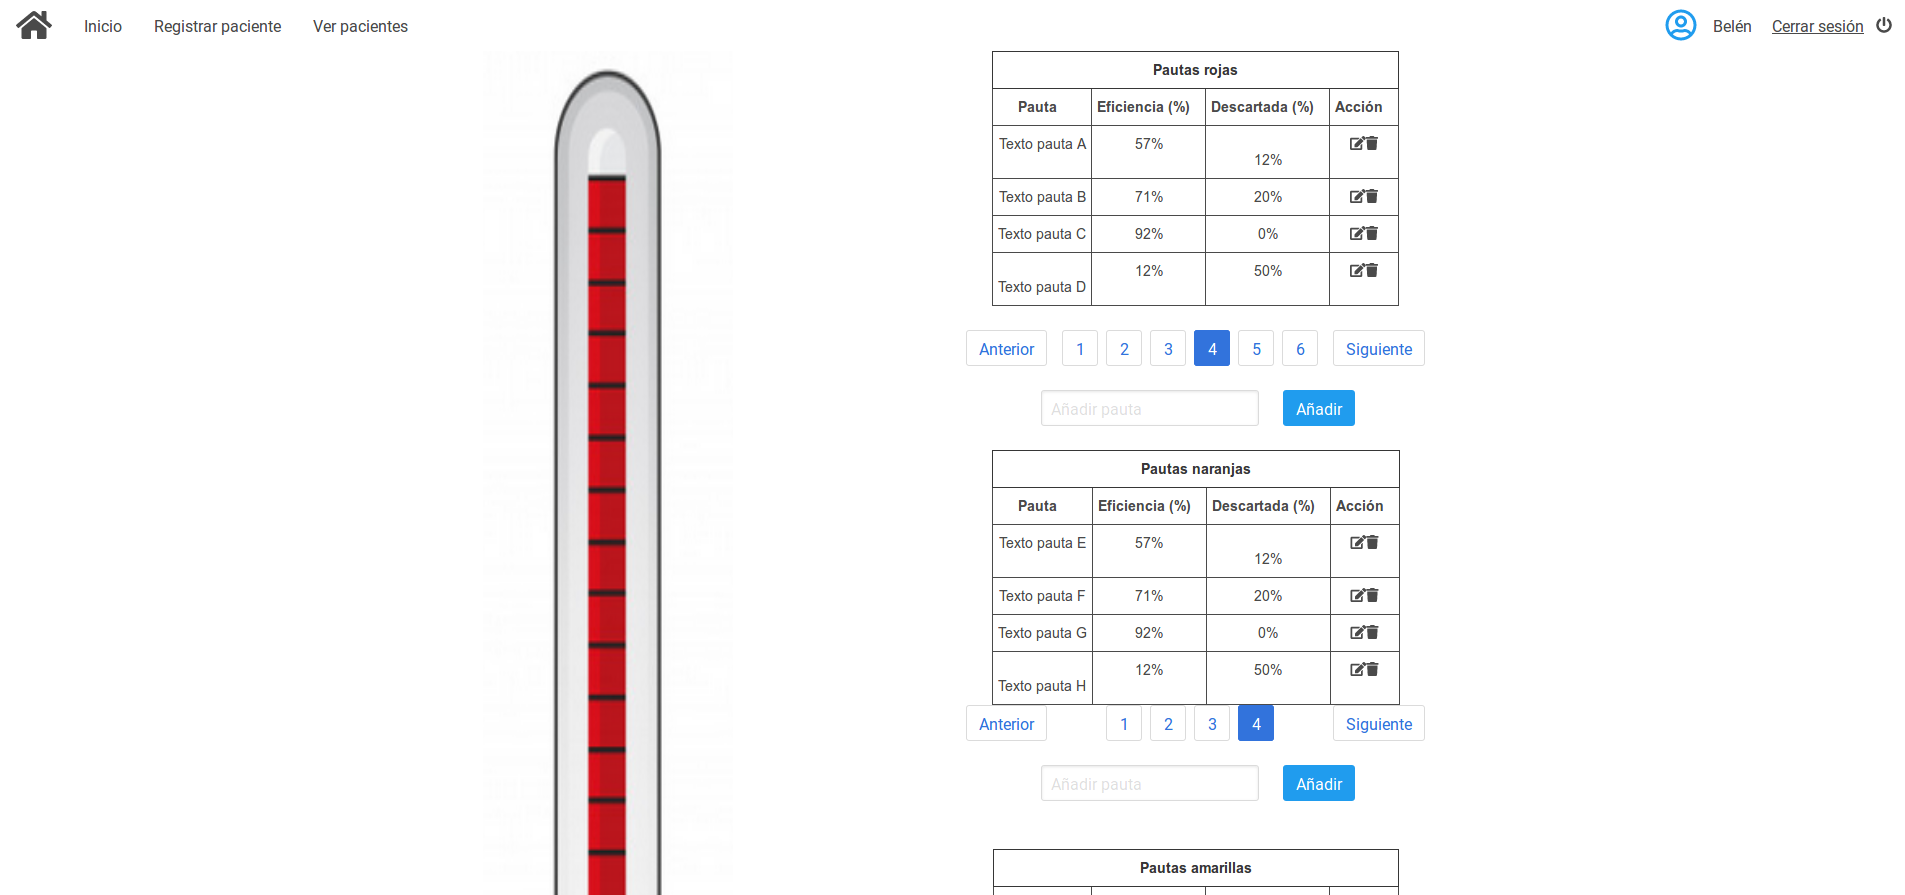
\includegraphics[height=7.5cm, width=\textwidth]{Imagenes/anxA20.png}
    \caption[Mockup de la pantalla para ver las pautas]{Mockup de la pantalla para ver las pautas}
    \label{fig:c4:mockup31}
\end{figure}

\paragraph{}
Tras la reunión con la terapeuta, los puntos que se sacaron en claro fueron los siguientes:

\begin{itemize}
    \item Las pantallas de las figura~\ref{fig:c4:mockup17} y~\ref{fig:c4:mockup18}  siguen teniendo en las tablas y en la gráfica alertas en lugar de eventos, por lo que los elementos que aparezcan en la web deben ser el conjunto de eventos del paciente en el que, al seleccionar algún episodio concreto, se pueda ver la información detallada de dicho episodio.
    \item La tabla de la figura~\ref{fig:c4:mockup18} debe ser interactiva. Se insiste en emular el diseño de los desfibriladores. La tabla de la figura~\ref{fig:c4:mockup19} que aparece debajo indicando las pautas seguidas en los distintos momentos es correcta, pero en el diseño final tiene que ser más detallada.
    \item La pantalla de la figura~\ref{fig:c4:mockup31} es una representación adecuada de las pautas almacenadas.
    \item Se echa en falta definir la pantalla en la que se añaden las pautas de cada paciente. En estas es necesario crear un sistema para poder heredar pautas de manera grupal para, a partir del paquete de pautas que se ha heredado, poder personalizarlas para cada paciente.
\end{itemize}

%TODO: esto probablemente acabe en otra sección mucho más detallada en la que se expliquen todos los aspectos técnicos de la solución final.
\section{Implementación}
\label{sec:c4:impl}
\paragraph{}
La pulsera es un dispositivo IOT que obtendrá las sensorizaciones del paciente cada [TODO] segundos. Concretamente, obtendrá los datos de sudoración, [TODO: constantes fisiológicas medidas]. Para ello, se ha elegido el modelo [TODO: modelo y descripción del modelo de la pulsera haciendo referencia a la comparación de pulseras del estado del arte].

\paragraph{}
Estas sensorizaciones se enviarán por BLE al dispositivo móvil con sistema operativo Android del paciente. La conexión será gestionada mediante una app creada para este proyecto, que irá guardando las sensorizaciones en una base de datos local de SQLite. La base de datos local estará encriptada con el algoritmo [TODO: rellenar cuando termine la app] para evitar dos posibles ataques: por un lado, si el paciente tiene el móvil \textit{rooteado} y la base de datos no está encriptada, si se instalase una aplicación maligna, esta podría acceder a los datos de la base de datos. Por otro, aunque el paciente no tuviera el móvil \textit{rooteado}, es necesario prevenir que estos datos se vieran expuestos si una tercera persona no autorizada tuviera acceso físico al mismo por ejemplo porque hubiese dejado desatendido su dispositivo temporalmente o le robasen el dispositivo.

\paragraph{}
En las aplicaciones móviles es crucial optimizar al máximo el uso de recursos para evitar que la aplicación creada interfiera con el normal funcionamiento del dispositivo ralentizándolo, consumiendo muchos datos o almacenando datos innecesarios. En esta línea, la aplicación borrará las sensorizaciones guardadas en local una vez hayan sido transformadas en episodios. Un episodio es un conjunto de sensorizaciones del paciente que muestran la transición del mismo desde que está calmado, se detecta la ira y vuelve al estado inicial. Como en el trabajo una vez transformada las sensorizaciones en posibles episodios esta información no es útil, se borra en cuanto se ha realizado esta conversión.

\paragraph{}
[TODO: expicar cuando esté la app de Android cómo se transforman las sensorizaciones en episodios.]

\paragraph{}
Por otro lado, los episodios del paciente sí persisten en la base de datos local de SQLite del dispositivo Android del paciente, ya que éste podrá acceder al archivo histórico de sus episodios para poder ver su progreso. Cada cinco minutos, se realizará una comunicación con el servidor para indicarle si en los últimos cinco minutos se han producido episodios de ira, y en cuyo caso se explicitará el episodio.

\paragraph{}
Como se ha comentado al principio de esta sección, cuando se detecte que el paciente pueda estar sufriendo un episodio de ira, se le proveerán de pautas en tiempo real que puedan ayudar a rebajar su nivel de ira. Las pautas recomendadas en ese momento podrán ser descartadas por el paciente y podrá añadir comentarios sobre la idoneidad de las mismas. Las pautas que aparezcan y la manera en la que el paciente interaccione con las mismas (si introduce comentarios, si las descarta, si han sido efectivas a la hora de rebajar el nivel de ira) será registrado en la base de datos local ya que esta información ayudará luego al terapeuta a ajustar mejor las pautas más adecuadas para cada paciente.

\paragraph{}
Estos datos se enviarán al servidor en formato JSON mediante el protocolo AMQP. Este es un protocolo de comunicación específicamente pensado para dispositivos IOT debido a su bajo consumo de recursos. Esta información estará cifrada usando el protocolo SSL para evitar robos de información sensible del paciente mediante técnicas de \textit{sniffing} o ataques de \textit{Man in the middle}.

\paragraph{}
Una vez llegan los datos de los posibles episodios y sus correspondientes pautas al servidor de AMQP, estos datos serán desencriptados y se persistirán en una base de datos de Mongo. El servidor contará con dos bases de datos: una base de datos SQLite que únicamente almacenará los credenciales de los terapuetas para acceder a la web y una base de datos de Mongo en el que se almacenará el resto de la información.

\paragraph{}
En la web el terapeuta podrá añadir nuevos pacientes, asociar pautas a pacientes en función de la intensidad de ira que se detecte y ver el histórico de episodios de cada paciente. Así, según las veces que se haya descartado una pauta, la efectividad de la misma o los comentarios de cada paciente, podrá modificar o eliminar la pauta para uno o más pacientes. Esto también sirve para poder comentar con el paciente los distintos episodios de ira que ha sufrido teniendo un registro histórico que pueda servir como referencia para guiar la terapia.
\cleardoublepage % Empty page before the start of the next part
%\include{Capitulos/05InteraccionUsuario}

%------------------------------------------------

\cleardoublepage % Empty page before the start of the next part

%----------------------------------------------------------------------------------------
%	THESIS CONTENT - APPENDICES
%----------------------------------------------------------------------------------------

%\appendix

%\part{Anexos} % New part of the thesis for the appendix

%\include{Anexos/01AnexoMockups}

%\include{Chapters/Chapter0A} % Appendix A
%\include{Chapters/Chapter0B} % Appendix B - empty template

%----------------------------------------------------------------------------------------
%	POST-CONTENT THESIS PAGES
%----------------------------------------------------------------------------------------

\cleardoublepage% Bibliography

\label{app:bibliography} % Reference the bibliography elsewhere with \autoref{app:bibliography}

\manualmark % Work-around to have small caps also here in the headline
\renewcommand\bibname{Bibliografía}
\markboth{\spacedlowsmallcaps{\bibname}}{\spacedlowsmallcaps{\bibname}} % Work-around to have small caps also
%\phantomsection
\refstepcounter{dummy}

\addtocontents{toc}{\protect\vspace{\beforebibskip}} % Place the bibliography slightly below the rest of the document content in the table of contents
\addcontentsline{toc}{chapter}{\tocEntry{\bibname}}

\printbibliography

%\cleardoublepage\include{Cascaras/Declaration} % Declaration
%\cleardoublepage\include{Cascaras/Colophon} % Colophon

%----------------------------------------------------------------------------------------

\end{document}
